%%%%%
%%
%% Sample document ``thesis.tex''
%%
%% Version: v0.2
%% Authors: Jean Martina, Rok Strnisa, Matej Urbas
%% Date: 30/07/2008
%%
%% Copyright (c) 2008-2011, Rok Strniša, Jean Martina, Matej Urbas
%% License: Simplified BSD License
%% License file: ./License
%% Original License URL: http://www.freebsd.org/copyright/freebsd-license.html
%%%%%

% Available documentclass options:
%
%   <all `report` document class options, e.g.: `a5paper`>
%   withindex   - enables the index. New index entries can be added through `\index{my entry}`
%   glossary    - enables the glossary.
%   techreport  - typesets the thesis in the technical report format.
%   firstyr     - formats the document as a first-year report.
%   times       - uses the `Times` font.
%   backrefs    - add back references in the Bibliography section
%
% For more info see `README.md`
\documentclass[withindex,glossary]{cam-thesis}

% Citations using numbers
\usepackage[numbers]{natbib}
\usepackage[T1]{fontenc}
\usepackage{textcomp}
\usepackage{graphicx}
\usepackage[spanish, activeacute]{babel} %Definir idioma español
\usepackage[utf8]{inputenc} %Codificacion utf-8
\usepackage{babel}
\usepackage{glossaries}
\usepackage{enumitem}
\usepackage{longtable}
\usepackage{glossaries}
\usepackage[export]{adjustbox}
\usepackage{siunitx}
\usepackage{color}
\usepackage{soul}
\usepackage{float}
\usepackage{titlesec}
\addto\shorthandsspanish{\spanishdeactivate{~<>}}
%%%%%%%%%%%%%%%%%%%%%%%%%%%%%%%%%%%%%%%%%%%%%%%%%%%%%%%%%%%%%%%%%%%%%%%%%%%%%%%%
%% Thesis meta-information
%%

%% Espacio entre párrafos:
\setlength{\parskip}{1em}

%%%%%%%%%%%%%%%%%%%%%%%%%%%%%%%%%%%%%%%%%%%%%%%%%%%%%%%%%%%%%%%%%%%%%%%%%%%%%%%%
%% Paragraph fomramt.
%%
\titleformat{\paragraph}
{\normalfont\normalsize\bfseries}{\theparagraph}{1em}{}
\titlespacing*{\paragraph}
{0pt}{3.25ex plus 1ex minus .2ex}{1.5ex plus .2ex}


%%%%%%%%%%%%%%%%%%%%%%%%%%%%%%%%%%%%%%%%%%%%%%%%%%%%%%%%%%%%%%%%%%%%%%%
%% The title of the thesis:
\title{Aspectos de Seguridad en la Interacción Humano-Robot Aplicados en un Robot Agropecuario.}

%% The full name of the author (e.g.: James Smith):
\author{Alberto Martinucci, Gonzalo Pelós}

%% College affiliation:
%\college{Facultado de Ingenieria, Universidad de la Republica}

%% College shield [optional]:
\collegeshield{images/fing_logo.png}

%% Submission date [optional]:
\submissiondate{Noviembre de 2017}

%% You can redefine the submission notice [optional]:
%\submissionnotice{A badass thesis submitted on time for the Degree of PhD}

\submissionnotice{Informe de Proyecto de Grado presentado al Tribunal
Evaluador como requisito de graduación de la carrera Ingeniería en Computación.
Montevideo, Diciembre de 2017.}

%% Declaration date:
\date{Diciembre, 2017}

%% PDF meta-info:
\subjectline{Computer Science}
\keywords{Robótica Agropecuario Seguridad}


%%%%%%%%%%%%%%%%%%%%%%%%%%%%%%%%%%%%%%%%%%%%%%%%%%%%%%%%%%%%%%%%%%%%%%%%%%%%%%%%
%% Abstract:
%%
\abstract{%
  My abstract ...
}


%%%%%%%%%%%%%%%%%%%%%%%%%%%%%%%%%%%%%%%%%%%%%%%%%%%%%%%%%%%%%%%%%%%%%%%%%%%%%%%%
%% Acknowledgements:
%%
\acknowledgements{%
  My acknowledgements ...
}

%%%%%%%%%%%%%%%%%%%%%%%%%%%%%%%%%%%%%%%%%%%%%%%%%%%%%%%%%%%%%%%%%%%%%%%%%%%%%%%%
%% Glossary [optional]:
%%
\newglossaryentry{HOL}{
    name=HOL,
    description={Higher-order logic}
}

\newglossaryentry{SBC}{
	name=SBC,
	description={Single Board Computer}
}


%%%%%%%%%%%%%%%%%%%%%%%%%%%%%%%%%%%%%%%%%%%%%%%%%%%%%%%%%%%%%%%%%%%%%%%%%%%%%%%%
%% Contents:
%%
\begin{document}

%%%%%%%%%%%%%%%%%%%%%%%%%%%%%%%%%%%%%%%%	%%%%%%%%%%%%%%%%%%%%%%%%%%%%%%%%%%%%%%%%
%% Title page, abstract, declaration etc.:
%% -    the title page (is automatically omitted in the technical report mode).
\frontmatter{}

%%%%%%%%%%%%%%%%%%%%%%%%%%%%%%%%%%%%%%%%%%%%%%%%%%%%%%%%%%%%%%%%%%%%%%%%%%%%%%%%
%% Thesis body:
%%
\chapter{Introducción}
Este capítulo presenta una introducción al proyecto de aspectos de seguridad e interacción humano-robot aplicados en un robot agropecuario. Incluye una exposición de las motivaciones para realizar el proyecto en la Sección 1.1, un resumen de los objetivos del proyecto en la Sección 1.2 y los aportes que se considera que el proyecto vuelca al conocimiento general de la temática en la Sección 1.3.

This is an example glossary reference: \gls{HOL}
 
%\marginpar[Margin note.]{Margin par.}

\section{Motivación} \label{sec: Introduccion :: Motivacion}
Si los robots van a ser introducidos en el mundo de los humanos para asistir o ayudar en la realización de una acción o tarea, dos problemas clave de los robots actuales deberán de ser solucionados. La interfaz robot-humano deberá ser de uso intuitivo y la seguridad del usuario, en lo que respecta a heridas infligidas por colisiones, deberá estar garantizada~\cite{Heinzmann2003}.

El robot DM3 tiene como objetivo asistir a humanos en tareas de recolección de frutos (peras y manzanas), esto es, el ambiente en el que el robot desempeñará su actividad será uno no estructurado y poblado por humanos. No cuenta, al inicio de este proyecto, con ningún mecanismo confiable que lo haga seguro.

\section{Aportes}
El objetivo de este trabajo consiste en investigar normas, guías y trabajos anteriores relacionados con aspectos de seguridad en robots autónomos que deban interactuar con humanos en ambientes abiertos y dinámicos, para luego implementar e incorporar un subconjunto de los mecanismos relevados al robot DM3.

Se dejan documentados los distintos mecanismos de seguridad implementados así como una guía de recomendaciones a seguir para garantizar la seguridad.

\chapter{Estado del Arte}
En esta sección se incluye un breve resumen del estado del arte. En la Sección 2.1 se presentan normas y estándares internacionales, finalmente, en la Sección 2.2 se describen aspectos de interacción humano-robot desde la perspectiva de la seguridad.

\section{Normas y Estándares Internacionales}
Durante la investigación inicial para la realización de este proyecto se estudiaron varias normas y estándares internacionales relacionados con la seguridad, algunos mas específicos que otros considerando el ámbito del proyecto. Se presenta brevemente las mas relevantes.

\subsection{ISO10218 - Robots y Dispositivos Robóticos, Requerimientos de Seguridad Para Robots Industriales} \label{sec: Marco Teorico :: Normas :: ISO 10218}
Especifica los requerimientos y pautas para un diseño seguro, medidas de protección e información para el uso de robots industriales. Describe peligros básicos asociados con los robots y proporciona los requisitos para eliminar, o reducir, los riesgos asociados a estos peligros. Aplica solo a los robots industriales, a pesar de esto los principios establecidos se pueden utilizar para otros tipos de robots. Se divide en dos partes ISO 10218-1 e ISO 10218-2, la primer parte aborda sólo el robot (manipulador y controlador) y la segunda parte aborda el sistema robótico y su aplicación.

Incluye las siguientes definiciones de interés:
\begin{itemize}[topsep=-11pt]
	\item \textbf{Robot colaborativo:} Aquel que puede ser utilizado en una operación colaborativa.
    \item \textbf{Operación Colaborativa:} En la parte 1, sección 3.4 la define como el estado en el cual robots, diseñados con un propósito, trabajan en cooperación directa con humanos en un espacio de trabajo definido, llamado espacio colaborativo.
    \item \textbf{Espacio Colaborativo:} En la parte 1, sección 3.5 lo define como el espacio de trabajo, dentro del espacio protegido, donde el robot y el humano pueden realizar tareas simultáneamente durante la operación de producción.
\\[-7pt]
\end{itemize}

En definitiva, de las definiciones anteriores se desprende que un robot colaborativo es definido por las tareas que realiza y el espacio donde estas tareas se realizan. No por características del robot en sí.

El Cuadro \ref{table:ISO10218_TiposOperacionColaborativa} presenta los distintos tipos de operación colaborativa e indica el principal medio por el cual es posible reducir el riesgo asociado al tipo de operación.
\begin{table}[H]
  \centering
  \begin{minipage}[b]{\textwidth}
  	\caption[ISO 10218-1, Tipos de Operación Colaborativa]{ISO 10218-1, Tipos de Operación Colaborativa}
  	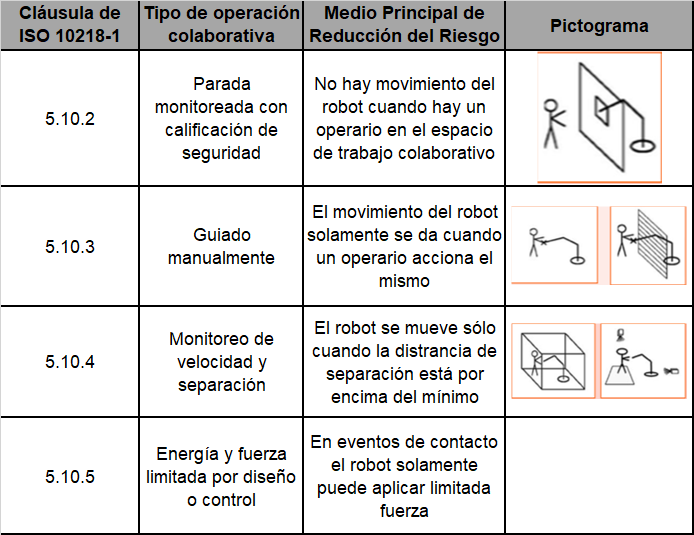
\includegraphics[width=\textwidth]{images/ISO10218_TiposOperacionColaborativa}  
  	\label{table:ISO10218_TiposOperacionColaborativa}
  \end{minipage}
\end{table}

\subsection{ISO/TS 15066 - Robots y Dispositivos Robóticos, Robots Colaborativos}
Especifica los requerimientos de seguridad para los sistemas robóticos industriales colaborativos y el ambiente de trabajo, complementa los requisitos y la orientación sobre la operación de robots industriales colaborativos dada por las normas ISO 10218-1 e ISO 10218-2. Al igual que la norma ISO 10218, es útil para robots no industriales aunque no especifica para estos.

Prescribe lineamientos de seguridad a seguir considerando las siguientes actividades:
\begin{itemize}[topsep=-11pt]
	\item Diseño de colaboración en el espacio.
    \item Diseño de la colaboración en la operación.
    	\begin{itemize}
    		\item Distancia mínima de separación y velocidad máxima del robot.
            \item Valores límites estáticos y dinámicos.
            \item Capacidades de sensado seguras.
            \item Ergonomía.
    	\end{itemize}
	\item Métodos de trabajo colaborativo.
    	\begin{itemize}
    		\item Guía a mano.
            \item Monitoreo de velocidad y separación.
            \item Límite de energía y  fuerza (criterio biomecánico).
    	\end{itemize}
	\item Cambios entre colaborativo y no colaborativo.
\\[-7pt]
\end{itemize}

Es de interés el criterio del límite biomecánico según el tipo de contacto que establece en la clausula 5.4.4 ``Limitación de potencia y fuerza'' que se presenta a continuación.

Tipo de evento de contacto:
\begin{itemize}[topsep=-11pt]
	\item Impacto libre o contacto transitorio (menos de \SI{50}{\milli\second}): Los parámetros a controlar son el peso y la velocidad del robot.
    \item Contacto por apretón o contacto casi estático: El parámetro a controlar es la fuerza.
\end{itemize}

\subsection{ISO 13482 - Robots y Dispositivos Robóticos, Requerimientos de Seguridad para Robots de Cuidado Personal}
Especifica los requerimientos y pautas para un diseño seguro, medidas de protección e información para el uso de robots para el cuidado personal, en particular, los siguientes tres tipos de robots; robot sirviente móvil, robot asistente físico y robot portador de persona. Complementa el estándar presentado en \ref{sec: Marco Teorico :: Normas :: ISO 10218}, que sólo abarca robots industriales.

Ofrece una caracterización de robots basada en sus atributos entre la cual se encuentra el tipo 3.2 que incluye a los robots personales móviles de ``múltiples pasajeros'' o ``pasajeros no de pie'' o ``al aire libre'' o ``superficies irregulares'' o ``no lento'' o ``no liviano'' o ``autónomo''. En esta categoría se podría incluir un robot como el DM3 a pesar de que este no sea uno de cuidado personal.

%No aplica a robots que se desplacen a velocidades superiores a los \SI{20}{\kilo\meter/\hour}.

\subsection{ISO 25119 - Tractores y Maquinaria para Agricultura y Silvicultura, Partes Relacionadas con la Seguridad de los Sistemas de Control}
Solo aborda el peligro para los humanos, y no para el robot. Cubre los posibles peligros causados por el comportamiento funcional de los sistemas relacionados con la seguridad, a diferencia de los riesgos que surgen de los propios equipos. Establece los principios generales para el diseño y desarrollo de las partes relacionadas con la seguridad de los sistemas de control en los tractores utilizados en la agricultura y la silvicultura, máquinas autopropulsadas de montar y máquinas montadas, semi-montadas y arrastradas utilizadas en agricultura.

\subsection{ANSI/RIA R15.06 - Instituto Nacional Estadounidense de Estándares para Robots Industriales y Sistemas Robóticos, Requerimientos Funcionales}
El estándar define disposiciones de consenso para la construcción, reconstrucción, modificación, instalación, protección, atención, pruebas y puesta en marcha de robots y sistemas robóticos, así como la formación operarios y personal de mantenimiento. Es la adopción estadounidense del estándar ISO 10218-1 e ISO 10218-2 y siendo esto así vale para este estándar lo comentado previamente en la sección \ref{sec: Marco Teorico :: Normas :: ISO 10218}.

\section{Seguridad en Interacción Humano-Robot}
Integrar robots en ambientes donde trabajan humanos es un tarea desafiante. Es importante reconocer que los usuarios que entablen interacciones humano-robot podrán enfrentar problemas y dificultades severas. Estos problemas y dificultades se extienden incluso más allá de los posibles daños, a humanos y materiales, que sean consecuencia de fallas; los estudios evidencian que las personas perciben a los robots autónomos de forma distinta a otras tecnologías informáticas~\cite{kiesler2004introduction}.

En las aplicaciones industriales, donde el uso de robots está extendido, la seguridad en la interacción humano-robot se lleva a cabo por medio del aislamiento del robot (en efecto, no hay interacción). De hecho, tanto el estándar estadounidense, ANSI/RIA 15.06~\cite{ANSIRIA1506}, como el europeo, EN-755~\cite{Gaskill1996}, contienen provisiones similares al respecto. En concreto, ambos indican que la seguridad es alcanzada definiendo una región al rededor del robot que debe ser custodiada, y que la acción a ser tomada por el sistema robótico al detectar una intrusión en dicha región es una parada de emergencia. Sin embargo, a medida que los robots se trasladan de estos ambientes industriales aislados a entornos interactivos, este enfoque deja de ser sostenible. De todas formas los conceptos asociados a la evaluación de los riesgos contenidos en estos estándares pueden aun ser aplicados.

Se reconocen 3 enfoques fundamentales para mitigar o eliminar riesgos: 
\begin{itemize}
\item Rediseñar el sistema para eliminar el peligro.
\item Controlar el peligro valiéndose de medios electrónicos o físicos.
\item Advertir al operador, ya sea durante la operación o por medio del entrenamiento.
\end{itemize}

La experiencia de la industria indica que el primer enfoque es el más exitoso como estrategia de reducción de riesgos~\cite{ANSIRIA1506}~\cite{IEC61508}. Este ha sido aplicado incluso en robots no industriales como pueden ser los presentados en ~\cite{Yamada1997}, ~\cite{Yamada1999} y ~\cite{Bicchia} que cuentan en su diseño con cobertura visco-eléctrica o articulaciones esféricas y flexibles.

\chapter{Marco Teórico}
Este capítulo presenta el marco teórico en el cual se encuadra el proyecto. En la Sección 3.1 se presenta el protocolo de comunicación HDLC, en la sección 3.2 se mencionan los aspectos básicos de la plataforma MCC, en la Sección 3.3 se describe el protocolo TCP, a continuación en la Sección 3.4 se describe brevemente Robot Operative System (ROS), y finalmente, en la Sección 3.5 se describen las características del Sistema Operativo de Tiempo Real (RTOS).

\section{High-Level Data Link Control}
Es un protocolo de comunicaciones de propósito general punto a punto, que opera a nivel de enlace de datos. Se basa en ISO 3309 e ISO 4335. Surge como una evolución del anterior SDLC. Proporciona recuperación de errores en caso de pérdida de paquetes de datos, fallos de secuencia y otros, por lo que ofrece una comunicación confiable entre el transmisor y el receptor. (\cite{RFC2687} \cite{RFC1662})

\subsection{Introducción}
El protocolo define detalladamente varios conceptos:
\begin{itemize}
\item \textbf{Estaciones - Terminales:}
	\begin{itemize}[label={--}]
	\item Estación primaria: controla el funcionamiento del enlace, y sus tramas se denominan órdenes.
    \item Estación secundaria: funciona controlada por la estación primaria, la que establece enlaces lógicos en cada una de las estaciones secundarias. Sus tramas se denominan respuestas.
    \item Estación combinada: usa tanto órdenes como respuestas.
	\end{itemize}
\item \textbf{Configuraciones del enlace:} permite semi-duplex y full-duplex
	\begin{itemize}[label={--}]
	\item Configuración no balanceada: una estación primaria y una o más secundarias.
    \item Configuración balanceada: consiste en dos estaciones combinadas.
	\end{itemize}
\item \textbf{Modos de transferencia de los datos:}
	\begin{itemize}[label={--}]
	\item Modo de respuesta normal: (NRM-“Normal response mode”) Se usa en la configuración no balanceada. La estación primaria puede iniciar la transferencia de datos a la secundaria, pero la secundaria sólo puede transmitir datos usando respuestas a las órdenes de la primaria.
    \item Modo balanceado asíncrono: (ABM-“Asynchronous balanced mode”) Se usa en la configuración balanceada, en la cual una estación combinada puede iniciar la transmisión sin necesidad de recibir permiso de la otra estación combinada.
    \item Modo de respuesta asíncrono: (ARM-“Asynchronous response mode”) Se usa en la configuración no balanceada. La estación secundaria puede iniciar la transmisión sin tener permiso explícito de la primaria, aunque ésta última sigue siendo la responsable del funcionamiento del enlace, incluyendo la iniciación, la recuperación de errores y la desconexión lógica.
	\end{itemize}
\end{itemize}
El modo NRM se usa en líneas con múltiples conexiones, con varios terminales conectados a un computador central, que sondea las entradas de cada terminal. En ocasiones se usa NRM en conexiones punto a punto. El ABM es el mas utilizado de los tres modos, ya que al no necesitar sondeos, los enlaces full duplex punto a punto son mas eficientes.
El ARM es el modo menos utilizado, reservado para los casos en que la estación secundaria requiere iniciar la transmisión.

\subsection{Estructura de la Trama}
HDLC utiliza transmisión síncrona, donde todos los intercambios se hacen a través de tramas, tanto para los datos como para la información de control.

\begin{figure}[H]
\centering
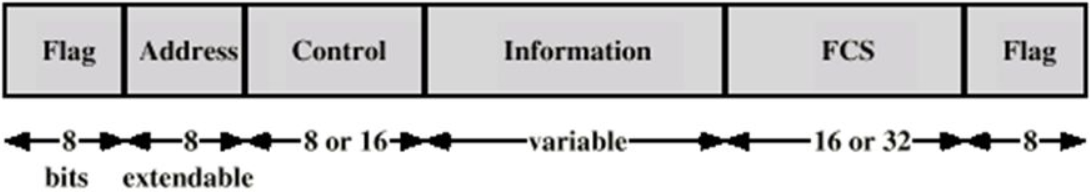
\includegraphics[width=0.5\textwidth]{images/HDLC_Frame}
\caption[Trama HDLC]{Trama HDLC.}
\end{figure}

\subsubsection{Campos de Delimitación}
En ambos extremos de la trama existen delimitadores de comienzo y final de trama (aunque podría haber uno solo). Es la combinación 01111110 que la estación receptora trata de detectar permanentemente, para establecer el comienzo y final de cada trama que recibe. Puede ocurrir que ésta misma secuencia exista dentro de la trama, lo que haría perder la sincronización a nivel de trama. Para evitarlo, se utiliza la técnica de “relleno de bits” (en inglés, “bit stuffing”), en la que el transmisor inserta un 0 tras toda cadena de cinco 1’s consecutivos si es que éstos no son de
algún delimitador de trama. El receptor, luego de haber detectado el inicio de una trama, si recibe cinco 1’s y luego un 0 sabe que éste último es solo de relleno, y lo descarta. Si el receptor recibe seis 1’s consecutivos, solamente los aceptará como un delimitador viniendo entre 0`s, ya que en caso contrario rechazará la trama por ser un error. Con el método de relleno de bits, los campos entre los delimitadores pueden contener cualquier secuencia arbitraria de bits, propiedad que se conoce como “transparencia de los datos”.

\begin{figure}[H]
\centering
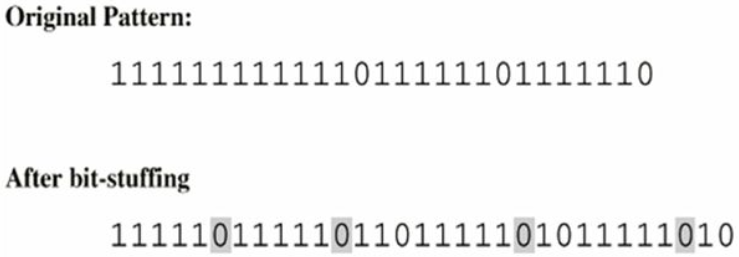
\includegraphics[width=0.5\textwidth]{images/HDLC_BitStuffing}
\caption[Relleno de bits de HDLC]{Relleno de bits de HDLC.}
\end{figure}

Si bien es común que las tramas utilicen delimitadores de comienzo y final, esto no es obligatorio en las especificaciones de HDLC.
El utilizar un solo delimitador de trama permite aprovechar mejor el enlace al enviar menor cantidad de bits de control, aunque la inversión de un bit, según donde se produzca, puede provocar que una trama se divida en dos, o eventualmente que dos tramas se fundan en una sola (siguiente imagen) y esto no ser detectado por el receptor. Con dos delimitadores por trama, éstas circunstancias serían rápidamente detectadas por el receptor.

\begin{figure}[H]
\centering
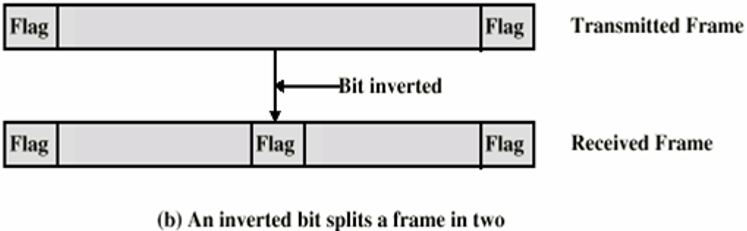
\includegraphics[width=0.5\textwidth]{images/HDLC_InvertedBit1}
\caption[Una inversión de bit divide la trama en 2]{Una inversión de bit divide la trama en dos.}
\end{figure}

\begin{figure}[H]
\centering
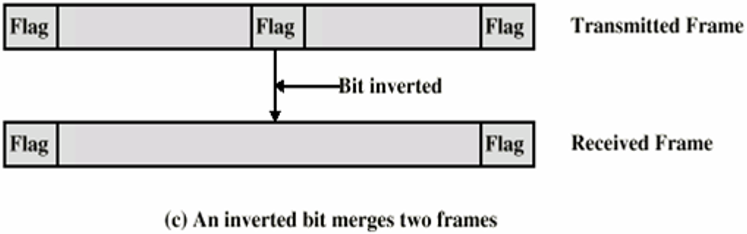
\includegraphics[width=0.5\textwidth]{images/HDLC_InvertedBit2}
\caption[Una inversión de bit fusiona dos tramas]{Una inversión de bit fusiona dos tramas.}
\end{figure}

\subsubsection{Campos de Dirección}
Identifica la estación secundaria que ha transmitido o que va a recibir la trama.
Por defecto tiene una longitud de 8 bits, aunque puede negociarse un formato ampliado en el que la dirección tenga una extensión múltiplo de 7 bits (el bit menos significativo de cada octeto en estado “1” indica que es el último octeto de la dirección ampliada; ese bit en estado “0” indica que hay mas octetos en la dirección). 

El octeto 11111111 comprende a todas las direcciones, tanto en el formato básico como en el ampliado, y se utiliza cuando la estación primaria quiere difundir una trama a todas las secundarias (broadcast).

\subsubsection{Campos de Control}
En HDLC se definen tres tipos de tramas, las que difieren solamente en el formato del campo de control.
\begin{itemize}
\item \textbf{Tramas-I} (“information”): transportan los datos generados por el usuario y la información para el control de flujo y control de errores.
\item \textbf{Tramas-S} (“supervisory”): procedimientos de confirmación cuando no es posible hacerlo en las tramas de información.
\item \textbf{Tramas-U} (“unnumbered” o no-numeradas): funciones suplementarias del control de enlace de datos.
\end{itemize}

El primer bit o los dos primeros del campo de control, identifican el tipo de trama, mientras los restantes se estructuran en sub-campos.

\begin{figure}[H]
\centering
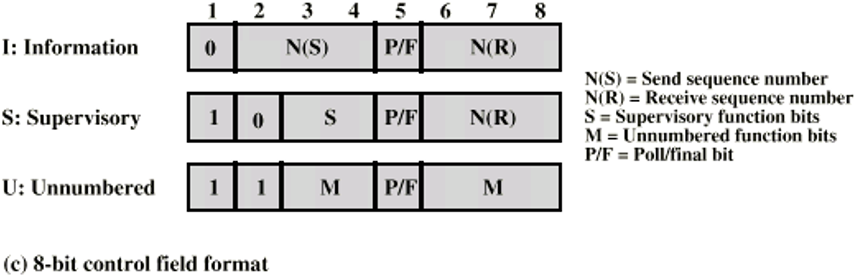
\includegraphics[width=0.5\textwidth]{images/HDLC_8BitCtrlField}
\caption[Formato de campo de control de 8 bits]{Formato de campo de control de 8 bits.}
\end{figure}

La figura anterior muestra el formato de campo de control de 8 bits, que maneja contadores para números de secuencias de tres bits, aunque se puede utilizar el formato extendido de siete bits, mediante la selección del modo extendido en la negociación inicial, con el formato de campos de la siguiente figura.

\begin{figure}[H]
\centering
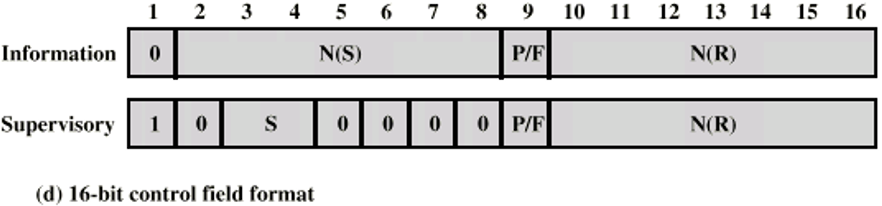
\includegraphics[width=0.5\textwidth]{images/HDLC_16BitCtrlField}
\caption[Formato de campo de control de 16 bits]{Formato de campo de control de 16 bits.}
\end{figure}

\subsubsection{Campos de Información}
Sólo presente en las tramas-I (y en algunas tramas-N). Puede contener cualquier secuencia de bits siempre que sea una secuencia de 8n bits, (n natural), por lo tanto con una longitud variable.

\subsubsection{Campo de Secuencia de Comprobación de Trama (FCS - Frame Check Sequence)}
Es un código de detección de errores, calculado sobre los bits de la trama, excluyendo los delimitadores. Se usa generalmente una CRC (Comprobación de redundancia cíclica) de 16 bits, y como opcional una de 32 bits.

\subsection{Funcionamiento}
Se lleva a cabo mediante el intercambio de tramas-I, tramas-S y tramas-U entre dos estaciones, que transportan órdenes y respuestas. Implica necesariamente tres fases: iniciación, transferencia de datos y desconexión.

\subsubsection{Iniciación}
Cualquiera de los extremos puede iniciar la transmisión, generando alguna de las seis posibles órdenes de modo. Esta orden cumple los siguientes tres propósitos:
\begin{itemize}
	\item Avisar al otro extremo que se ha solicitado la iniciación.
    \item Especificar el modo solicitado (NRM, ABM o ARM)
    \item Especificar si se utilizaran números de secuencia de 3 ó 7 bits.
\end{itemize}
Si la solicitud del transmisor se acepta, el receptor envía una trama de confirmación no numerada (UA-“unnembered acknowledged”). Si la solicitud se rechaza, el receptor envía una trama de modo desconectado (DM - “disconnected mode”).

\subsubsection{Transferencia de Datos}
Con la iniciación solicitada y aceptada, se habrá establecido la conexión lógica. Ambos lados pueden comenzar a enviar datos mediante tramas-I, comenzando con el número de secuencia 0. La secuencia de tramas-I se numeran secuencialmente módulo 8 ó módulo 128, según se utilice 3 ó 7 bits respectivamente, utilizando el campo N(S).

El campo N(R) se utiliza para la confirmación de las tramas-I recibidas, por lo que se indica al otro extremo el número de la próxima trama que se espera recibir (“reconocimiento inclusivo”). 

Las \textbf{tramas-S} también se utilizan para el control de flujo y errores:
\begin{itemize}
	\item RR: confirma la última trama-I recibida (implica la próxima que aguarda. Se usa cuando no hay tráfico de de tramas-I en el otro sentido).
    \item RNR: confirma la última trama-I recibida, pero solicita interrumpir los envíos de tramas. Cuando esté listo listo, enviará una RR.
    \item REJ: rechaza la última trama-I recibida, y solicita la retransmisión de todas las tramas-I numeradas a partir de N(R).
    \item SREJ: rechaza una trama específica, de la cual solicita retransmisión.
\end{itemize}

\subsubsection{Desconexión}
Cualquiera de los extremos puede solicitar la desconexión, ya sea por iniciativa propia (detección de un fallo) o por solicitud de una capa superior. HDLC lleva a cabo la desconexión transmitiendo una trama de desconexión (DISC), a la que el otro extremo responderá con una UA.

\subsection{Ejemplos de Operación}
En los diagramas siguientes, cada fila especifica el nombre de la trama. Cuando se requiere, se dan los contenidos de V(S) y de V(R). El bit P/F (“poll/final”) se fija en 0, salvo cuando explícitamente aparece, que estará indicado en 1.

%\subsubsection{Iniciación del enlace y desconexión}
%\begin{minipage}{0.3\textwidth}
%\begin{figure}[H]
%\centering
%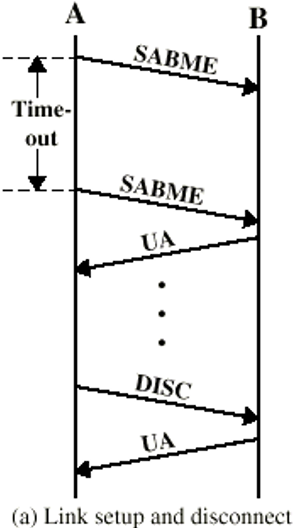
\includegraphics[width=\textwidth]{images/HDLC_SetupDisconnect}
%\caption[Establecimiento de enlace y desconexión]{Establecimiento de enlace y desconexión.}
%\end{figure}
%\end{minipage}
%\begin{minipage}{0.6\textwidth}%\raggedleft
%	\begin{itemize}
%		\item A envía SABM y activa un temporizador. B responde con UA, inicializa sus %variables de estado y contadores. Ambos quedan listos para iniciar el intercambio de %tramas.
%		\item Si B no respondiera al SABM dentro del tiempo del temporizador, A insistirá %hasta obtener de B una respuesta UA ó DM. Si no respondiera el ETD B a pesar de los %intentos, A avisaría a las capas superiores.
%		\item Finalmente se ilustra la desconexión.
%	\end{itemize}
%\end{minipage} 

\subsubsection{Iniciación del enlace y desconexión}

\begin{figure}[H]
\centering
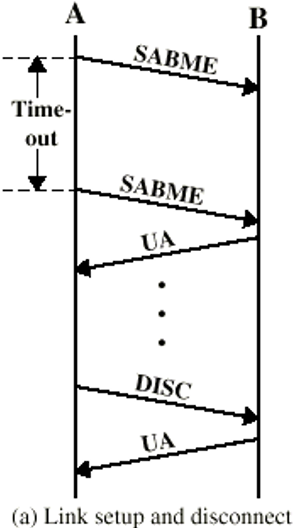
\includegraphics[height=7.0cm]{images/HDLC_SetupDisconnect}
\caption[Establecimiento de enlace y desconexión]{Establecimiento de enlace y desconexión.}
\end{figure}

\begin{itemize}
	\item A envía SABM y activa un temporizador. B responde con UA, inicializa sus variables de estado y contadores. Ambos quedan listos para iniciar el intercambio de tramas.
	\item Si B no respondiera al SABM dentro del tiempo del temporizador, A insistirá hasta obtener de B una respuesta UA ó DM. Si no respondiera el ETD B a pesar de los intentos, A avisaría a las capas superiores.
	\item Finalmente se ilustra la desconexión.
\end{itemize}

\subsubsection{Intercambio de datos en ambos sentidos}

\begin{figure}[H]
\centering
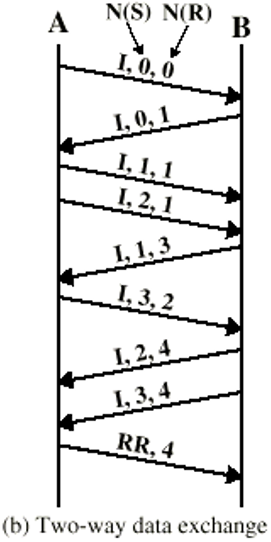
\includegraphics[height=7.0cm]{images/HDLC_TwoWay}
\caption[Intercambio de datos bidireccional]{Intercambio de datos bidireccional.}
\end{figure}

Los siguientes puntos suponen ya superada la iniciación del enlace:
\begin{itemize}
	\item La trama I con N(S) = 1 y N(R) = 3 es un ejemplo de reconocimiento inclusivo.
	\item La última trama-S, RR, se envía de A hacia B ya que el primero no posee tramas-I para enviar con datos.
\end{itemize}

\subsubsection{Condición de receptor ocupado}

\begin{figure}[H]
\centering
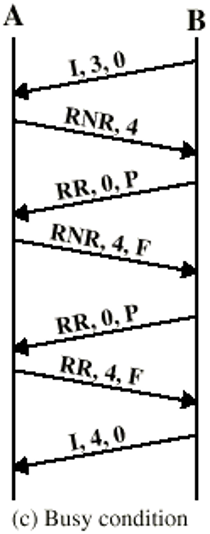
\includegraphics[height=7.0cm]{images/HDLC_BusyCondition}
\caption[Condición de ocupado]{Condición de ocupado.}
\end{figure}

Los buffers del receptor se pueden desbordar porque HDLC puede ser incapaz de procesar las tramas-I a la velocidad que le llegan, o bien porque el usuario no puede recibirlas tan rápidamente (p.ej. limitación de una impresora).
\begin{itemize}
	\item Envía RNR confirmando la última trama recibida, pero solicitando una pausa en el envío.
	\item B sondeará periódicamente a A con RR (bit P = 1).
	\item Cuando A está listo, envía RR (bit P = 0).
\end{itemize}

\subsubsection{Recuperación de un rechazo}

\begin{figure}[H]
\centering
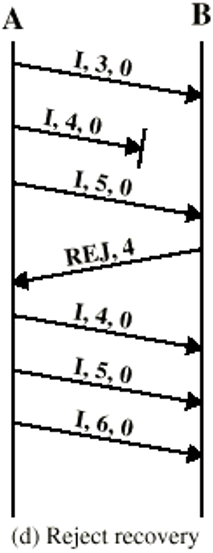
\includegraphics[height=7.0cm]{images/HDLC_RejectRecovery}
\caption[Recuperación de Rechazo]{Recuperación de Rechazo.}
\end{figure}

\begin{itemize}
  \item La trama-I número 4, enviada por A se pierde por un error.
  \item B rechaza la trama 5, ya que esperaba la 4.
  \item Envía REJ4, por lo que A retransmite todas las tramas desde la 4 inclusive, y posteriores.
\end{itemize}

\subsubsection{Recuperación de un error utilizando temporizadores}

\begin{figure}[H]
\centering
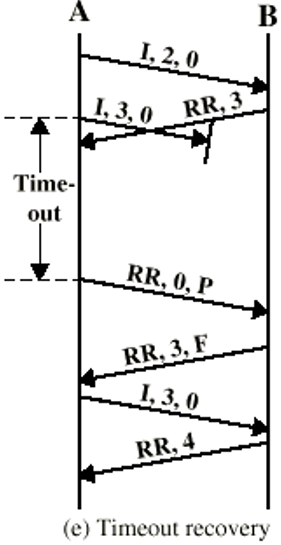
\includegraphics[height=7.0cm]{images/HDLC_TimeoutRecovery}
\caption[Recuperación por Timeout]{Recuperación por Timeout.}
\end{figure}

\begin{itemize}
  \item A envía una secuencia de tramas a B, perdiéndose la número 3, que era la última de la transmisión de A.
  \item El ETD B detecta el error, pero no puede mandar hacia A una REJ, ya que no puede saber si la trama que se perdió es tipo I.
  \item A había iniciado un temporizador al enviar la trama I,3,0 por lo que vencido el mismo, sondeará con RR (P/F con P = 1).
  \item Al responder B con el número de trama que espera recibir, el A sabe que debe retransmitir la I,3,0 y se evita el dead-lock.
\end{itemize}

\section{MCC} \label{sec: Marco Teo :: MCC}
\subsection{Introducción}
\textit{Micro Contoller Controller} es un protocolo desarrollado por el grupo MINA de la Facultad de Ingeniería \cite{GRUPOMINA}, para el envío de mensajes entre un host y un micro-controlador. El mismo corre sobre un enlace serial o TCP y es asíncrono, en el que tanto el host como el micro-controlador pueden emitir mensajes y se minimiza el tráfico de datos debido a que éstos están en el medio únicamente cuando son de interés para alguna de las partes. 

\subsubsection{Procesos}
Cada módulo del micro-controlador y el host representan un proceso (o servicio) direccionable de forma individual mediante un identificador único llamado \textit{pid}.
MCC ofrece una API que consiste en la definición de la estructura de mensajes que pueden ser transferidos. La interfaz define un conjunto de métodos, que se identifican por un código llamado \textit{opcode}, y un conjunto de parámetros. 
Algunos de los \textit{opcodes} son reservados y tienen una semántica predefinida que es contemplada por un proceso encargado de administrar a la placa micro-controlador y a todas las tareas. 
Los procesos ofrecen un mecanismo uniforme para brindar meta información sobre si mismos, de ésta manera es posible interrogar a un proceso sobre su API.

\subsubsection{Enlace}
El medio de comunicación entre el host y la placa micro-controladora donde se intercambian mensajes.
Los mensajes pueden ser originados en el host o en alguno de los procesos del micro-controlador. El protocolo no prevé una respuesta obligatoria a los mensajes, pero esta puede ser provista a nivel de implementación de los procesos y especificada en su API.

\subsubsection{Mensajes}
El mensaje es la unidad de información intercambiada entre el host y los procesos del mircro-controlador. Son enviados en texto plano, codificados utilizando bencode \cite{BENCODE}. Esta codificación es un mecanismo de serialización que permite representar estructuras de datos simples, generando representaciones en texto plano donde los procesos de codificación y decodificación son muy eficientes, ya que no necesitan memoria para almacenar resultados intermedios.
Los mensajes pueden ser dos tipos:
El protocolo es asimétrico (maestro-esclavo), donde los mensajes soportados en la dirección host $\rightarrow$ micro-controlador son distintos a los que van en la dirección opuesta. No obstante el protocolo es regular y los mensajes son funcionalmente equivalentes.

\textbf{Mensajes originados en el host}: van dirigidos a un método y proceso particular del microcontrolador y tienen la siguiente estructura: $[ target\_pid, opcode, data]$
\begin{itemize}
	\item \textit{target\_pid}: identificador, de tipo numérico, del proceso del micro-controlador al que va dirigido el mensaje.
     \item \textit{opcode}: identificador,de tipo numérico, del método del proceso del micro-controlador que debe procesar el mensaje.
     \item \textit{data}: conjunto de parámetros, de tipo caracteres representados en 8bit-clean, para el método a invocar en el micro-controlador. 
\end{itemize}

\textbf{Mensajes originados en un proceso del micro-controlador}: provienen de un proceso en particular y contienen datos que serán reportados al host y tienen la siguiente estructura: $[ source\_pid, opcode, data]$
\begin{itemize}
	\item \textit{source\_pid}: identificador, de tipo numérico, del proceso del microcontrolador que genera el mensaje.
    \item \textit{opcode}: identificador,de tipo numérico, del método del proceso del microcontrolador que genera el mensaje.
	\item \textit{data}: conjunto de datos, de tipo caracteres representados en 8bit-clean, que se reportan al host. 
\end{itemize}
\section{TCP}
El protocolo de control de transmisión (en inglés \textbf{T}ransmition \textbf{C}ontrol \textbf{P}rotocol), es uno de los protoclos fundamentales en Internet, definido en los documentos RFC 793 \cite{TCPRFC793}, RFC 1122 \cite{TCPRFC1122}, RFC 1323 \cite{TCPRFC1323}, RFC 2018 \cite{TCPRFC2018} y RFC 2581 \cite{TCPRFC2581}. 

Es un protocolo de la capa de transporte de Internet fiable y orientado a la conexión, donde antes de que un proceso de la capa aplicación pueda comenzar a enviar datos a otro, los dos procesos deben primero establecer una comunicación entre ellos; es decir, tienen que enviarse ciertos segmentos preliminares para definir los parámetros de la transferencia de datos que llevarán a cabo luego.

Una conexión TCP proporciona un servicio full-duplex, esto es, dada una conexión TCP entre el proceso A que se ejecuta en un host y el proceso B que se ejecuta en otro host, los datos de la capa de aplicación pueden fluir desde el proceso A al proceso B en el mismo instante que los datos de la capa de aplicación fluyen del proceso B al proceso A. Además el protocolo garantiza que los datos serán entregados en su destino, sin errores y en el mismo orden en que se transmitieron.

\section{Robot Operating System (ROS)}
El Sistema Operativo de Robots (en inglés Robot Operating System, ROS), es un meta-sistema operativo de código abierto para robots. Provee servicios que uno esperaría de un sistema operativo, incluyendo abstracción del hardware, control de dispositivos de bajo nivel, implementación de funcionalidades comúnmente usadas, intercambio de mensajes entre procesos y gestión de paquetes. También provee herramientas y librerías para obtener, compilar, codificar, y ejecutar código a través de múltiples computadoras \cite{wikiROS}.

\begin{figure}[H]
  \centering
  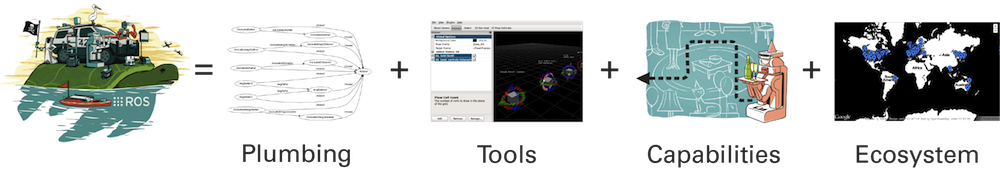
\includegraphics[width=\textwidth]{images/ros_equation}
  \caption[Ecuación de ROS]{Ecuación de ROS.}
\end{figure}

ROS no remplaza a los sistemas operativos tradicionales sino que trabaja junto con estos. Esto presenta la pregunta de porque utilizar ROS entonces, cuando aprender un nuevo marco de trabajo es una tarea difícil, y ROS es particularmente complejo y diverso. Para responder esa pregunta a continuación se presenta algunos puntos específicos sobre el desarrollo de software para robots que ROS puede ayudar a resolver.

\begin{itemize}
  \item Computación Distribuida: Muchos sistemas robóticos modernos dependen de software que abarca muchos procesos diferentes y ejecuta  en varias computadoras diferentes, lo cual presenta la necesidad de comunicación entre estos procesos. ROS provee dos mecanismos para llevar adelante esta comunicación, la publicación de mensajes en tópicos y las llamadas a servicios.
  \item Reutilización de Software: El rápido progreso de la investigación robótica ha resultado en una creciente colección de buenos algoritmos para resolver tareas comunes como la navegación, la planificación de movimientos, la construcción de mapas y muchas otras. La existencia de estos algoritmos solo es verdaderamente útil si hay una forma de aplicarlos en nuevos contextos sin la necesidad de reimplementarlos para cada nuevo sistema. ROS ayuda a prevenir este problema en al menos dos formas, los paquetes estándar de ROS proveen una implementación estable y \textit{debuggeada} de muchos algoritmos importantes y el pasaje de mensajes propuesto por ROS se ha vuelto el estándar \textit{de facto} para la interoperabilidad de software robótico. Esto resulta en que comúnmente se encuentren disponibles para ROS interfaces al hardware mas moderno e implementaciones de los algoritmos más avanzados.
  \item Testeo Rápido: Una de las razones por las cuales el desarrollo de software para robots es mas complejo que otras clases de desarrollo es que el testeo puede consumir mucho tiempo y es propenso a errores. Es posible que muchas veces no se cuente con el robot físico para trabajar con el, y cuando esta disponible el trabajo es lento y delicado. Utilizar ROS provee dos soluciones a este problema. Sistemas que utilicen ROS, bien diseñados, separan el control de bajo nivel del hardware, el procesamiento de alto nivel y la toma de decisiones en programas distintos, esta separación permite sustituir los programas de bajo nivel por simuladores, lo cual permite testear los componentes de alto nivel del sistema. ROS provee una forma simple de grabar y reproducir datos de sensores y otros mensajes, esto significa que se puede obtener mas beneficios del tiempo en el que se tenga físicamente disponible el robot ya que grabando la información de los sensores luego es posible reproducirla y testear distintas formas de procesar los mismos datos. En la jerga de ROS estas grabaciones son llamadas \textit{bags} y una herramienta llamada \textit{rosbag} es la que se utiliza para grabar y reproducirlas.
\end{itemize}

Cabe destacar que ROS no es la única plataforma en ofrecer estas capacidades, sin embargo existe un apoyo generalizado a ROS en el ámbito de la robótica y una gran comunidad al rededor del mismo. Esta ``masa crítica'' de apoyo hace que sea razonable pensar que ROS seguirá evolucionando, expandiéndose y mejorando en el futuro. Esta es una fuerte razón para elegir ROS a la hora de seleccionar un marco de trabajo.

\section{Sistema Operativo de Tiempo Real (RTOS)}\label{sec: Marco Teórico - RTOS }
Los sistemas embebidos son plataformas con escasos recursos en comparación con una PC, sin embargo las aplicaciones de microcontroladores modernas frecuentemente deben ejecutar varias tareas concurrentemente, esto es llamado multi-tarea. En realidad, cada núcleo de un procesador solo puede correr un hilo de ejecución a la vez. Una parte del sistema operativo llamada planificador es responsable de decidir que programa correr y cuando, provee la ilusión de ejecución simultanea mediante el rápido intercambio entre las tareas.

El tipo de un sistema operativo, en el sentido de si es de tiempo real o no, es definido por como el planificador decide que programa ejecutar. Por ejemplo el planificador utilizado en un sistema operativo multiusuario (como Unix) se asegurara de que a cada usuario le sea otorgada una cantidad justa de tiempo de procesamiento. Como otro ejemplo, el planificador de un sistema operativo en una PC de escritorio (como Windows) tratara de asegurarse de que la computadora permanezca responsiva al usuario. 

El planificador en un RTOS está diseñado para proveer un patrón de ejecución predecible (normalmente descrito como determinista). Esto es de particular interés para los sistemas embebidos ya que como característica común generalmente incluyen en su especificación de requerimientos información de tiempos límite (\textit{deadlines}) que debe ser cumplida, esto es, tienen restricciones de tiempo real. Una restricción de tiempo real es una que especifica que el sistema embebido debe responder a un cierto evento en un lapso de tiempo estrictamente definido (el \textit{deadline}). Solo se puede garantizar el cumplimiento de los requerimientos de tiempo real si se puede predecir el comportamiento del planificador del sistema operativo.

Existen dos filosofías de diseño principales para los planificadores de un RTOS:	
\begin{itemize}[topsep=-11pt]
  \item Guiada por eventos: Cambia de tarea solo cuando un evento de mayor prioridad necesita ser atendido; llamada prioridad con derecho preferente (\textit{preemptive priority}), o planificación por prioridad (\textit{priority scheduling}).
  \item Tiempo compartido: Cambia de tareas en interrupciones de reloj regulares, y en eventos; llamada por turnos (\textit{round robin}). \\[-7pt]
\end{itemize}

Los algoritmos mas comunes de planificación son:
\begin{itemize}[topsep=-11pt, noitemsep]
  \item Planificador Expropiativo:
  	\begin{itemize}[topsep=-11pt, noitemsep]
  	  \item Planificador de tasa monotónica: Asigna prioridades fijas a las tareas. La asignación se hace en función de la duración de la tarea, las tareas mas cortas tienen las prioridades mas altas. 
      \item Planificador por turnos: Todas las tareas tienen la misma prioridad. Se define una porción de tiempo (\textit{time slice}) durante el cual una tarea puede ejecutar durante cada turno. Si la tarea finaliza su ejecución, cambia a estado en espera o consume toda la porción de tiempo asignada el planificador comienza a ejecutar la siguiente tarea lista para ejecutar.
      \item Planificador Expropiativo de Prioridad Fija: Las tareas tienen prioridad fija. Cada tarea ejecuta durante una porción de tiempo luego de la cual el planificador expropia el uso del procesador, la siguiente tarea a ejecutar sera la de mas alta prioridad que este lista. Este comportamiento puede hacer que tareas de prioridad baja esperen indefinidamente, para remediar esto se puede ir incrementando la prioridad de las tareas en espera a medida que pasa el tiempo de forma que eventualmente sean seleccionadas por el planificador para ejecutar.
  	\end{itemize}
  \item Planificador Cooperativo: Confía en que cada tarea ceda regularmente tiempo a las otras tareas del sistema. Puede sufrir de inanición si una tarea mal programada no cede el control, por esta afirmación no debería emplearse en un sistema de tiempo real. Sin embargo sí se puede considerar el uso este planificador, ya que permite obtener comportamiento \textit{soft real-time} y mediante el uso de interrupciones y otros mecanismos cumplir con los requerimientos \textit{hard real-time}, en escenarios en los cuales utilizar un RTOS es excesivo con las ventajas de que este planificador es simple de implementar, \textit{debuggear} y consume poca memoria flash y RAM.
  \item Planificador de Menor Tiempo de Respuesta Primero: Las prioridades de las tareas son dinámicas. Al momento de realizar un cambio de tarea este planificador seleccionara aquella tarea lista mas próxima a finalizar, por ejemplo asignando prioridades inversamente proporcionales al tiempo restante para finalizar. Tiene las ventajas de que no hay necesidad de definir las prioridades de las tareas de antemano, en general realiza menos cambios de contexto y es posible aprovechar el procesador al 100\%. Como desventajas se puede mencionar que es menos predecible (el tiempo de respuesta de las tareas es variable), brinda menos control sobre la ejecución (no es posible cambiar la prioridad de las tareas a demanda), tiene un mayor costo de implementación y es muy difícil computar el tiempo de respuesta. \\[-7pt]
\end{itemize}

Cabe destacar que el tipo de planificador comúnmente encontrado en los sistemas de tiempo real es una combinación del planificador expropiativo de prioridad fija y el planificador por turnos. Esto es, cada vez que el planificador deba seleccionar una tarea para ejecutar tomará aquella de máxima prioridad, y de haber varias con la misma prioridad máxima ejecutará estas tareas por turnos.

Las tareas (\textit{tasks}), que forman las unidades lógicas de computación en un procesador, son sobre con las cuales opera el planificador, decidiendo cual es la siguiente a ejecutar y asignando el procesador a la misma. Si bien no es deseable violar los límites de tiempo de las tareas de un sistema de tiempo real, estas pueden ser más o menos valiosas (considerando lo que los resultados de su ejecución aportan al sistema) o críticas para el sistema, y de esto dependerán las consecuencias del no cumplimiento de los límites de tiempo. Considerando esto, las tareas pueden ser clasificadas en uno de los tres tipos que se presentan a continuación.

\begin{itemize}[topsep=-11pt]
	\item Tarea de tiempo real duro (\textit{Hard real-time task}): Si la tarea no es finalizada antes de su tiempo límite, aunque sea una sola vez, se debe considerar que el sistema ha fallado. Debe estar determinado y acotado con exactitud el tiempo en el cual ejecutan estas tareas, e incluso las latencias de interrupción y cambio de contexto. El sistema de airbags de un vehículo es un claro ejemplo de este tipo de tarea, el sistema debe desplegar los airbag en el momento exacto y de no hacerlo (tanto si los despliega temprano como tarde) el resultado será desastroso.
    \item Tarea de tiempo real blando (\textit{Soft real-time task}): Para estas tareas los tiempos límites deben ser en su mayoría cumplidos, pero se acepta el incumplimiento de unos pocos sin que el resultado de esto sea considerado falla del sistema. Para estas tareas solo se define la precedencia y secuencia de las operaciones que realizan, las latencias de interrupción y cambio de contexto son pequeñas pero puede haber desviaciones entre las esperadas y las observadas. El resultado de la ejecución de la tarea se sigue considerando útil aún cuando se ha obtenido luego del tiempo límite, la acumulación de no cumplimientos de tiempos límites para estas tareas resultará en la degradación de la calidad del servicio del sistema. Un sistema de transmisión de audio y video en vivo es un ejemplo de este tipo de tareas, las restricciones de tiempo deben cumplirse para que el audio y el video estén sincronizados, violaciones a las restricciones temporales que no ocurran frecuentemente no afectan gravemente la calidad de la transmisión pero una acumulación de estas resultaría en audio y video notablemente fuera de sincronía.
    \item Tarea de tiempo real firme (\textit{Firm real-time task}): Al igual que para las tareas de tiempo real blando, si no es frecuente, el no cumplir con el límite de tiempo establecido para la tarea no implica una falla del sistema, incluso si el no cumplimiento es reiterado. Sin embargo, a diferencia de estas el resultado de la tarea carece de valor si es obtenido luego del tiempo límite (la utilidad del resultado es 0 luego del \textit{deadline}). Un ejemplo de tarea de este tipo se puede encontrar en sistema de manufactura con líneas que cuenten con robots para el ensamblado, en estos el no cumplir con un tiempo límite resultará en el ensamblado incorrecto de la pieza. Pero mientras la ocurrencia de piezas mal ensambladas sea infrecuente y no muy costosas la producción continuará.
\\[-7pt]
\end{itemize}

Informalmente, un sistema de tiempo real crítico para la seguridad puede ser definido como uno en el cual el daño resultante por no cumplir una restricción de tiempo de una tarea es mayor que cualquier beneficio que pueda ser obtenido por una ejecución correcta y oportuna de esta. Adicionalmente, un sistema se puede definir como de tiempo real duro si el daño tiene el potencial de ser catastrófico, esto es, las consecuencias son inconmensurablemente mayores que cualquier beneficio provisto por el sistema en ausencia de fallas \cite{audsley1990real}.

Ademas de la gestión de tareas y el planificado descritos anteriormente, en general los RTOS ofrecen también servicios de gestión de la memoria, comunicación entre procesos, sincronización de procesos, manejo de interrupciones y \textit{timers}.

\chapter{Guía de Seguridad para Robots Colaborativos}
En el presente capitulo se intentará desarrollar una guía de seguridad que sirva como primer referencia durante el desarrollo de un robot autónomo y colaborativo. Sin ser exhaustiva incluirá recomendaciones, puntos a los que prestar especial atención, protocolos, técnicas y buenas practicas a aplicar con el propósito de eliminar los peligros y riesgos existentes allí donde sea posible, o reducirlos al mínimo donde no, en pos de salvaguardar la integridad física tanto de humanos como robots. 

Primero en la sección \ref{sec: Guía Seguridad :: Diseño y Construcción} se tratara el diseño y la construcción del robot, a continuación en la sección \ref{sec: Guía Seguridad :: Instalación y Explotación} se mencionaran aspectos a tener en cuenta durante las etapas de instalación y explotación del robot en el ambiente y, para finalizar, en la sección \ref{sec: Guía Seguridad :: Técnicas Seguridad} se enumeraran técnicas de software de referencia.

\section{Diseño y Construcción} \label{sec: Guía Seguridad :: Diseño y Construcción}
\textbf{Acceso al Panel de Control Principal:} Debe haber un panel de control del robot ubicado fuera del área de trabajo del mismo, si esta está bien definida, si no, debe haber una base de control que sea siempre accesible a los operarios.

\textbf{Kill Switch:} Al menos un mecanismo de parada de emergencia, fácilmente reconocible y de fácil acceso. La identificación de estos mecanismos es fundamentales en la formación de operarios. Deben tener prioridad sobre cualquier otro control.

\textbf{Identificación de Dispositivos de Control:} Todos los dispositivos de control (botones, switches, palancas, etc.) deberán estar claramente identificados y etiquetados de forma que sea fácil reconocerlos y entender su propósito.

\textbf{Dispositivo de Arranque o Alimentación de Energía:} Los dispositivos de arranque o alimentación de energía deberán tener un diseño tal que no sea posible accionarlos involuntariamente. El bloqueo de estos dispositivo solo debe ser posible en la posición de apagado.

\textbf{Comunicación con Operarios:} Utilizar pantallas que presenten indicaciones a los operarios para minimizar los errores que estos puedan cometer. Informar el estado del robot.

\textbf{Dispositivos de Detección de Presencia:} Sensores externos al robot, colocados en el ambiente que aporten información acerca de la ubicaciones de personas. Los mas comúnmente usados son las esteras de presión, las cortinas de luz, sensores capacitivos, ultrasonidos, sensores de radiofrecuencia, láser, cámaras, etc.

\textbf{Sistemas de Alerta Audible y Visible:} Sistemas de alerta audible y visible para complementar otros métodos de salvaguarda (detección de presencia, barreras, etc.). Estas alertas deben ser claramente reconocibles.

\textbf{Movilidad segura del robot:} El diseño del robot debe ser tal que pueda ser movido libremente sin necesidad encenderlo ni alimentarlo con corriente.

\textbf{Frenos mecánicos adicionales:} Si el robot maneja grandes cargas o su peso es significativo, debería contar con frenos adicionales que se activen cuando se corte la alimentación a los actuadores. Se debe disponer de mecanismos para desactivar estos frenos de forma manual.

\section{Diseño de Software} \label{sec: Guía Seguridad :: Diseño de Software}
\begin{itemize}
  \item Proveer la capacidad de parar el sistema automáticamente frente a velocidades anormales desarrolladas por componentes del robot al llevar a cabo sus tareas.
  \item Incluir técnicas de prevención de colisiones y minimización del impacto frente a accidentes.
    \begin{itemize}
        \item Prevención del accidente: Uso de sensores ubicados en puntos estratégicos para considerar el volumen del robot y un área virtual de alto riesgo. Esto acompañado de algoritmos que permiten tomar decisiones frente a posibles colisiones.
        \item En caso de accidente: El sistema deberá estar preparado para actuar de manera que minimice el impacto (fuerzas repulsivas, torque, etc.).
    \end{itemize}
  \item El acceso a la unidad de control, el arranque, parada y modificación del programa deben estar restringidos mediante algún mecanismo de seguridad (llaves, códigos de acceso, etc.)
  \item Contemplar mecanismos de recuperación frente a fallas. Considerar sistemas de control alternativos, respaldo.
  \item El sistema de control debe supervisar continuamente el correcto funcionamiento de componentes y sub-sistemas, incluyendo la supervisión del propio sistema de control, esto ultimo por ejemplo utilizando un watchdog timer.
\end{itemize}

\section{Instalación y Explotación} \label{sec: Guía Seguridad :: Instalación y Explotación}
\subsection{Consideraciones Generales}
\begin{itemize}
  \item Considerar y seguir rigurosamente todas las especificaciones de los fabricantes.
  \item Permitir únicamente a personal calificado operar con el robot.
  \item Instalar mecanismos de seguridad para acceder al sistema del robot (códigos acceso al sistema).
  \item Identificar claramente la zona de trabajo del robot y sus movimientos. Proporcionar sistemas para controlar al robot fuera de su zona de trabajo (e.g.: parada de emergencia).
  \item Controlar periódicamente todos los equipos y conexiones de seguridad que resulten ser críticos.
  \item Contar con señales luminosas y acústicas que indiquen el correcto funcionamiento del robot y que llamen la atención cuando haya riesgo de accidente.
  \item Cortar la alimentación y neutralizar todos los dispositivos de almacenamiento de energía del robot durante el proceso de ajuste o reparación de algún componente.
  \item De existir una etapa de aprendizaje para el sistema robótico, solo deberán tener el control del robot desarrolladores y personal capacitado mientras dure.
  \item No superar velocidades de \SI{250}{\milli\metre/\second} $=$ \SI{0.9}{\kilo\metre/\hour} en las etapas de producción y puesta en marcha. Realizar pruebas progresivas aumentando las velocidades paulatinamente hasta lograr ejecutar de manera continua y a las velocidades finales deseadas.
\end{itemize}

\subsection{Operarios}
\begin{itemize}
  \item Contar con personal designado como administradores o supervisores cuya responsabilidad sea hacer cumplir las políticas de seguridad.
  \item Procurar que el personal entienda la tarea completa para la cual esta programado el robot antes de comenzar a operar con él. 
  \item Quien sea responsable por los robots deberá asentar por escrito que asegura que todo el personal es consciente de las políticas de seguridad y está capacitado para cumplirlas.
  \item Brindar a los operarios una formación adecuada en el reconocimiento de riesgos y peligros, del equipo y de procedimientos adecuados para operar el robot.
  \item Si se requiere realizar el entrenamiento de operarios colaborando con el robot y compartiendo el espacio de trabajo, se ha de realizar a bajas velocidades y habiendo dado a conocer previamente los mecanismos de parada de emergencia y componentes que alimentan de energía al robot.
  \item Permitir que solo personal especializado realice operaciones de programación y mantenimiento.
\end{itemize}

\subsection{Ambiente}
Diseñar el robot contemplando las condiciones ambientales a las cuales podrá estar sometido al momento de realizar las tareas. En caso de exposición a la intemperie considerar factores como la humedad, presión atmosférica, polvo, lluvia, etc. que podrán variar repentinamente, el robot debe estar preparado para actuar en buena forma frente a estas eventualidades.

Analizar las posibles condiciones ambientales de operación al momento de seleccionar sensores para el robot, para así garantizar que estos funcionaran correctamente en todas ellas. De no ser posible, disponer de sensores redundantes que sean capaces de medir la misma magnitud física en distintas condiciones y/o aplicar técnicas de fusión.

Para el caso particular de los dispositivos de visualización (cámaras) sera de gran importancia contemplar los diferentes niveles de iluminación bajo los cuales deberá operar el robot.

\section{Técnicas de Seguridad} \label{sec: Guía Seguridad :: Técnicas Seguridad}
\begin{itemize}
\item Supervisión de Funciones: Supervisión básica del movimiento del robot, i.e: el movimiento ejecutado se corresponde con el movimiento comandado. Supervisión de las cantidades cinemáticas como son la posición, velocidad, aceleración y frenado. Supervisión de cantidades dinámicas como lo son el torque y la fuerza. Funciones de supervisión definidas por el usuario, relacionadas con la aplicación.
\item Recuperación Frente a Fallas:\hl{FALTA}
\item Prevención de Colisiones:
  \begin{itemize}
  	\item 3D Sensor Fusión: Fusión en tiempo real de información provista por sensores de imagen tridimensional para crear una representación del espacio a través de una grilla de evidencia volumétrica (\textit{volumetric evidence/occupancy grid}). Se segmenta el espacio en fondo, robots y humanos. Al rededor del robot se define una zona de peligro y al rededor de cada persona o todo aquello que se quiera proteger se define una zona de seguridad. Si estas zonas se intersecan el robot se debe enlentecer o detener hasta que la situación se resuelva. \hl{PONER REFERENCIAS A APLICACIONES}
    \item Predicción de Movimiento y Acción Humana: Bajo este titulo se engloban varias técnicas que persiguen como fin otorgar al robot la capacidad de inferir o predecir movimientos y acciones humanas. Ya sea esto para evitar accidentes o asistir en la realización de tareas. 
  \end{itemize}
\item Estrategias de Control de Colisiones:
  \begin{itemize}
    \item Control de Torque con Compensación de la Gravedad: \hl{FALTA}
    \item \hl{OTROS?? EL QUE IMPLEMENTAMOS??}
  \end{itemize}
\item Estrategias de Control:
  \begin{itemize}
  	\item Campo de Peligro Cinetoestático: Este concepto captura en una única medida el estado completo del robot, su configuración y velocidad. Se intenta con este método  estimar el peligro en la vecindad del robot. Se puede considerar una generalización del enfoque de campos de potenciales para la búsqueda de trayectorias, con el cual difiere en que captura la velocidad y postura del robot, y en que la fuente del campo de potenciales es el robot mismo en lugar de los humanos/obstáculos.
    \item \hl{OTRO?} \hl{LA QUE UTILIZA EL DM3?? Va mas por el lado de computar y seguir un camino virtual o buscar un objetivo?}
  \end{itemize}
\item Códigos de Acceso al Sistema: Se recalca la importancia que tiene que el acceso a la unidad de control, el arranque, parada y modificación del programa, deben estar limitados mediante el empleo de algún mecanismo de seguridad (llaves, códigos de seguridad, etc.).
\end{itemize}

\chapter{Solución Propuesta}
En este capítulo se plantea la solución al problema abordado en el proyecto. En la Sección 4.1 se detallan los requerimientos del sistema, en la Sección 4.2 se muestra la arquitectura de la solución, en la Sección 4.3 se presenta y justifica los protocolos de comunicación empleados, en la Sección 4.4 se presentan y describen los mecanismos de seguridad desarrollados e integrados al DM3 y por último en la Sección 4.5 el se describe el método utilizado para comunicar el estado del robot a los usuarios.

\section{Requerimientos} \label{sec:Sol Prop :: Requerimientos}
Si bien no se recibimos requerimientos funcionales explícitos, construimos el siguiente conjunto de requerimientos como resultado de la investigación realizada durante el revelamiento del estado del arte.

\begin{itemize}
	\item Establecer criterios de lo que es el funcionamiento normal y seguro del robot (distancias, velocidades y potencias) y velar por que estos se cumplan.
	\item Desarrollar mecanismos de bajo nivel (en comparación con los implementados en la SBC) para garantizar que el robot no colisione con obstáculos.
	\item Implementar un mecanismo por el cual se comunique al usuario el estado del robot.	
	\item El protocolo de comunicación entre la SBC y la placa de entrada/salida debe proveer mecanismos que hagan frente a la pérdida de paquetes, errores de secuencia y arribos de paquetes fuera de orden, con el propósito de que la comunicación entre los nodos sea confiable.
	\item Incluir el uso de Watchdog timer.
\end{itemize}

Como requerimientos de \textit{hardware} inicialmente se solicitó que la placa seleccionada tuviese como mínimo las siguientes características:
\begin{itemize}
    \item Interfaz Serial/USB.
    \item Interfaz de comunicación serial síncrona y asíncrona. Soportar I2C.
    \item Al menos 6 salidas digitales, 4 para direcciones de ruedas, freno, habilitación, luz de seguridad y bocina.
    \item 4 salidas analógicas, podrían ser PWM con filtros pasa bajo como se describe en \cite{AN538}.
    \item Entradas para la señal de los sensores hall.
    \item Servicio de WatchDog Timer (WDT).
\end{itemize}
Luego se determinó que los motores utilizados, ver \ref{sec: Implementación :: Plataforma Utilizada - Hardware - Actuadores}, eran muy sensibles como para funcionar con PWM, requiriéndose una salida analógica real e independiente para cada  uno. Ninguna de las placas evaluadas cuenta con 4 salidas analógicas por lo cual se decidió utilizar un \hl{DAC} externo (ver Sección \ref{sec: Implementación :: Plataforma Utilizada - Hardware - Otros}) controlado con el protocolo \hl{I2C}.

\section{Arquitectura de la Solución}

En la definición de la arquitectura propuesta para el sistema de control del robot tenemos un conjunto de módulos, elementos de software y hardware involucrados. La implementación de los módulos de hardware y la interconexión entre ellos y los elementos de software definen dicha arquitectura.
Ofrece los medios por los cuales el sistema puede lograr sus metas eficientemente, satisfacer restricciones de tiempo real, promover la tolerancia a fallas y proporcionar seguridad para el robot y su entorno. Debe ofrecer una distribución apropiada para los procesos de sensado y procesamiento de manera que éstos se realicen en tiempos razonables para conseguir los objetivos propuestos.

\subsection{Requerimientos}

\subsection{Componentes}

\begin{figure}[H]
\centering
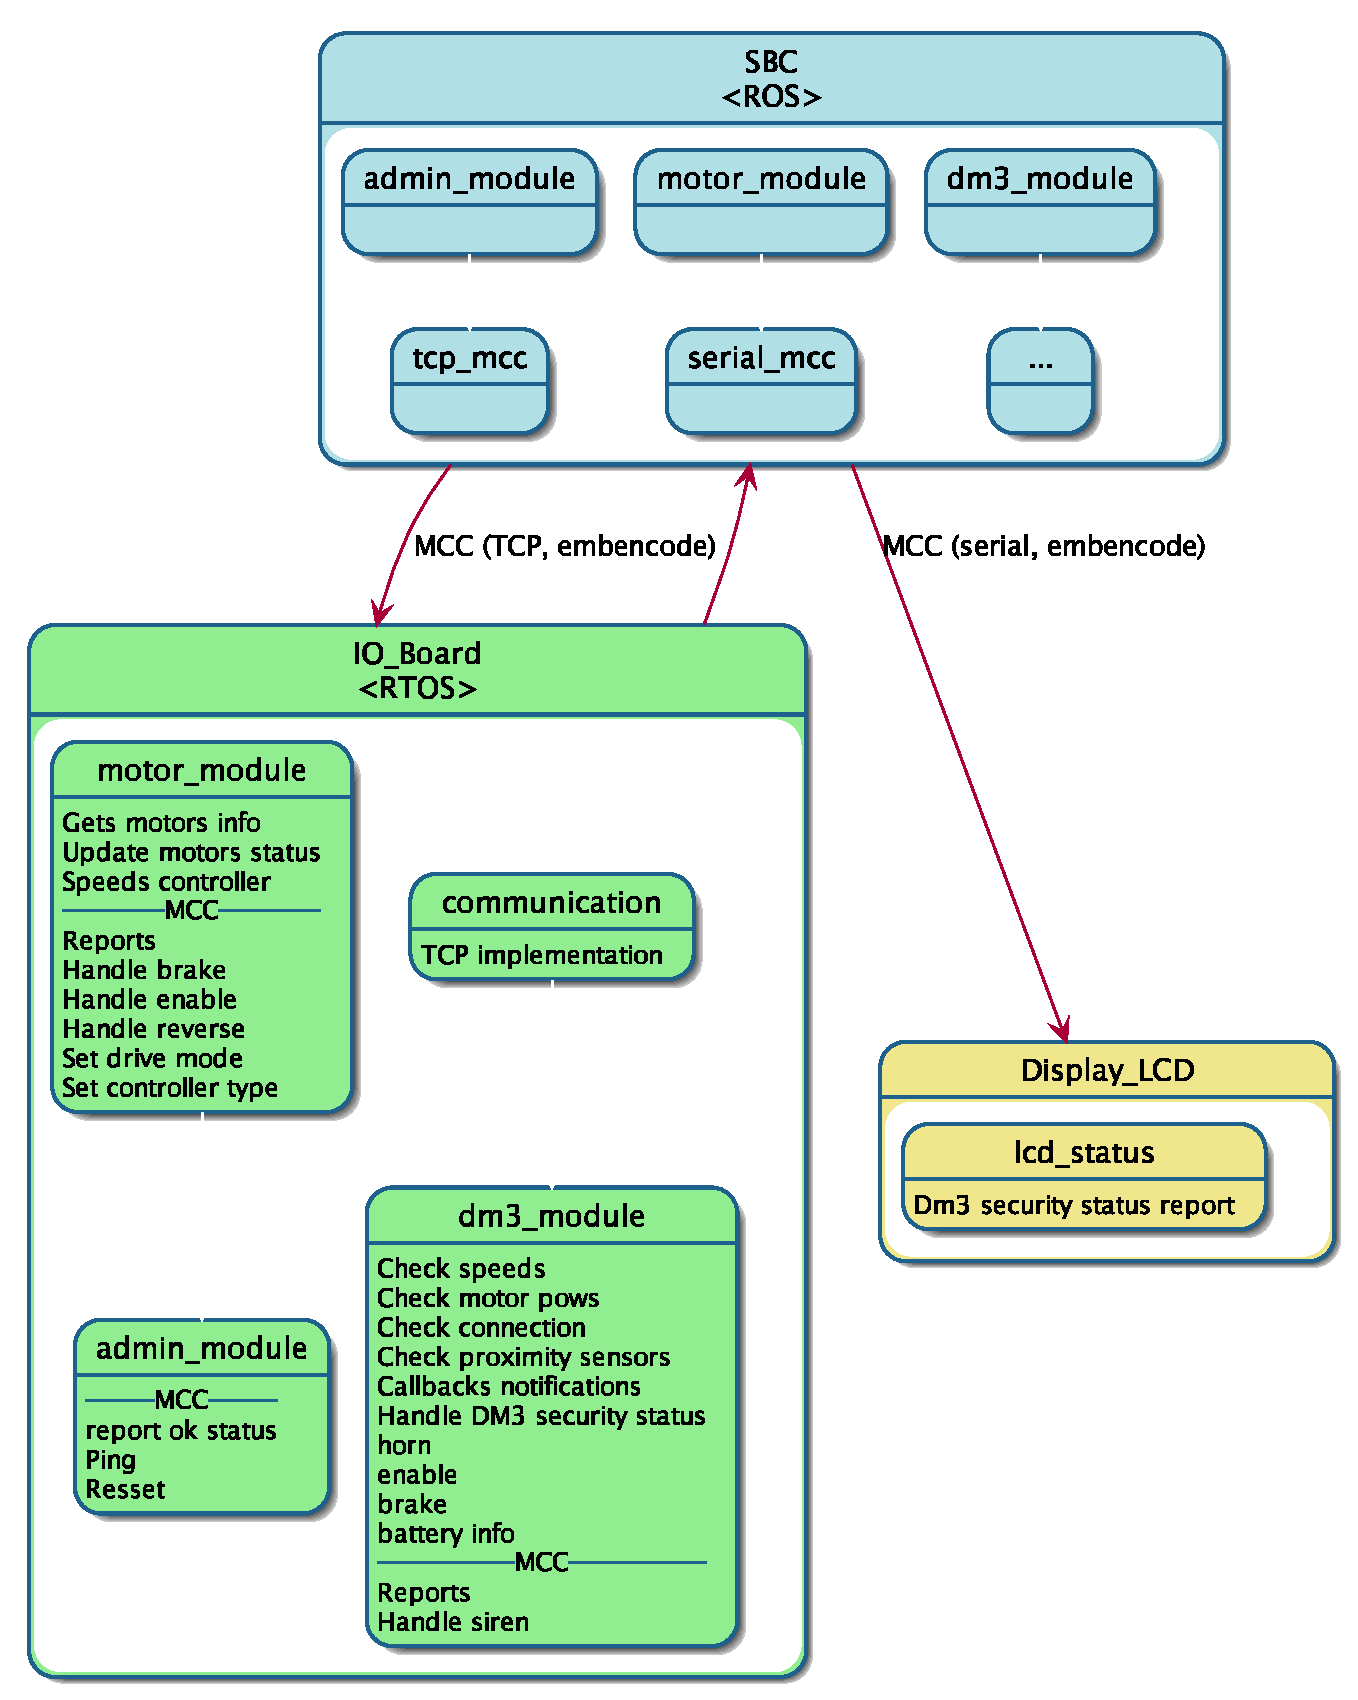
\includegraphics[width=0.5\textwidth]{images/DM3_Modules}
\caption[Diagrama de componentes de módulos]{Diagrama de módulos - Firmware k64F.}
\end{figure}

\subsubsection{SBC}
El robot cuenta con una \gls{SBC} Odroid dedicada a procesar el stack de navegación y la detección de obstáculos. Esta placa es el cerebro del robot y se comunica con una placa de entrada/salida, mediante el protocolo MCC sobre TCP, para comandar el funcionamiento del robot y obtener información de los diferentes componentes de hardware como ser: 
\begin{itemize}
	\item Velocidad actuales y deseadas en las diferentes ruedas.
	\item Potencias establecidas y deseadas en los motores.
	\item Estados de frenos
	\item Nivel de carga de las baterías
	\item Estado de seguridad del robot.
\end{itemize}

También se comunica con una display para mostrar un reporte de estados de seguridad del robot.
A continuación se comenta sobre los módulos de la \hl{SBC} que han tenido más participación en el desarrollo de este proyecto.

\paragraph{tcp\_mcc} \label{sec:Sol Prop :: tcp_mcc}
Este nodo ROS es el encargado de establecer y mantener activa la comunicación con la placa K64F, mediante un socket TCP, implementando operaciones para enviar y recibir información.

\paragraph{serial\_lcd}
Nodo ROS encargado de reenviar reportes de estados, recibidos desde el modulo descrito en \ref{sec:Sol Prop :: admin_module}, hacia la placa Odroid Show para que ésta placa los presente en un display LCD. La comunicación entre las placas mencionadas es controlada por este nodo e implementada sobre una conexión serial USB.

\paragraph{motor\_module}
Módulo responsable de controlar los motores del robot así como también  de generar reportes con información relevante a velocidades, potencias y estados. Implementa operaciones para enviar comandos, vía MCC sobre TCP, a la placa de entrada salida para:
\begin{itemize}
	\item (des)habilitar los motores	
	\item (des)habilitar el freno	
	\item establecer velocidades a los motores
	\item (des)habilitar la reversa
	\item establecer potencias a los motores
	\item establecer el tipo de controlador de los motores
	\item establecer el tipo de manejo de los motores
\end{itemize}

\paragraph{admin\_module} \label{sec:Sol Prop :: admin_module}
Módulo que recibe y procesa reportes de estados y errores que envía la placa de entrada salida mediante la conexión MCC sobre la conexión TCP establecida, también recibe el estado de la conexión desde el nodo ROS descrito en \ref{sec:Sol Prop :: tcp_mcc}. Mantiene el estado de los distintos dispositivos y mecanismos de seguridad así como el estado general del firmare corriendo en la placa \hl{IOBoard}. El reporte de estados es presentado en la placa \hl{Display\_LCD}, ésta placa recibe dicho reporte a través de una comunicación en un canal serial USB utilizando códigos de escape ANSI/VT100.

También son implementadas en este módulo las operaciones de ping y reset de la placa \hl{IOBoard}. La operación ping envía un mensaje MCC a la placa K64F y espera recibir un paquete con la misma información desde dicha placa. Por otra parte la operación reset envía un mensaje MCC a la placa K64F indicando que debe ser reiniciada.

\paragraph{dm3\_module}
Este módulo recibe y reporta el estado de la batería del robot, así como también implementa la funcionalidad de activación de una sirena; para ello envía un mensaje MCC a la placa de entrada/salida y ésta es la encargada de (des)activar la sirena al procesar el mensaje.

\subsubsection{Display LCD}
Placa que recibe un reporte de información de estados del robot desde la placa Odroid a través de una conexión serial USB, procesa la información recibida y la presenta en un display LCD. Este reporte es de gran utilidad para los operarios y muy importante desde el punto de vista de la seguridad en el trabajo cooperativo humano-robot debido a que en el mismo se indican los estados de los diferentes componentes de hardware:
\begin{itemize}
\item estado general del robot
\item estado de conexión TCP entre las placas Odroid y K64F
\item estado de control de potencias de los motores
\item estado de control de velocidades de los motores
\item estado de control de sensores de proximidad
\end{itemize}

\subsubsection{IO Board}
El módulo más importante desarrollado en este proyecto es la unidad de control que maneja todos los sensores de bajo volumen de datos así como también a los motores del robot.
Para desarrollar la unidad de control se utiliza una placa \hl{IOBoard} que proporciona los recursos necesarios para desarrollar un sistema basado en RTOS (ver \ref{sec: Marco Teórico - RTOS }) que procese la información y tome acciones en tiempo real.

Para explicar con un poco más de detalle, a continuación se presenta un diagrama con los componentes presentes en la placa \hl{IOBoard} y a partir de éste describiremos cómo se relacionan unos con los otros y cuales son sus responsabilidades.

\begin{figure}[H]
\centering
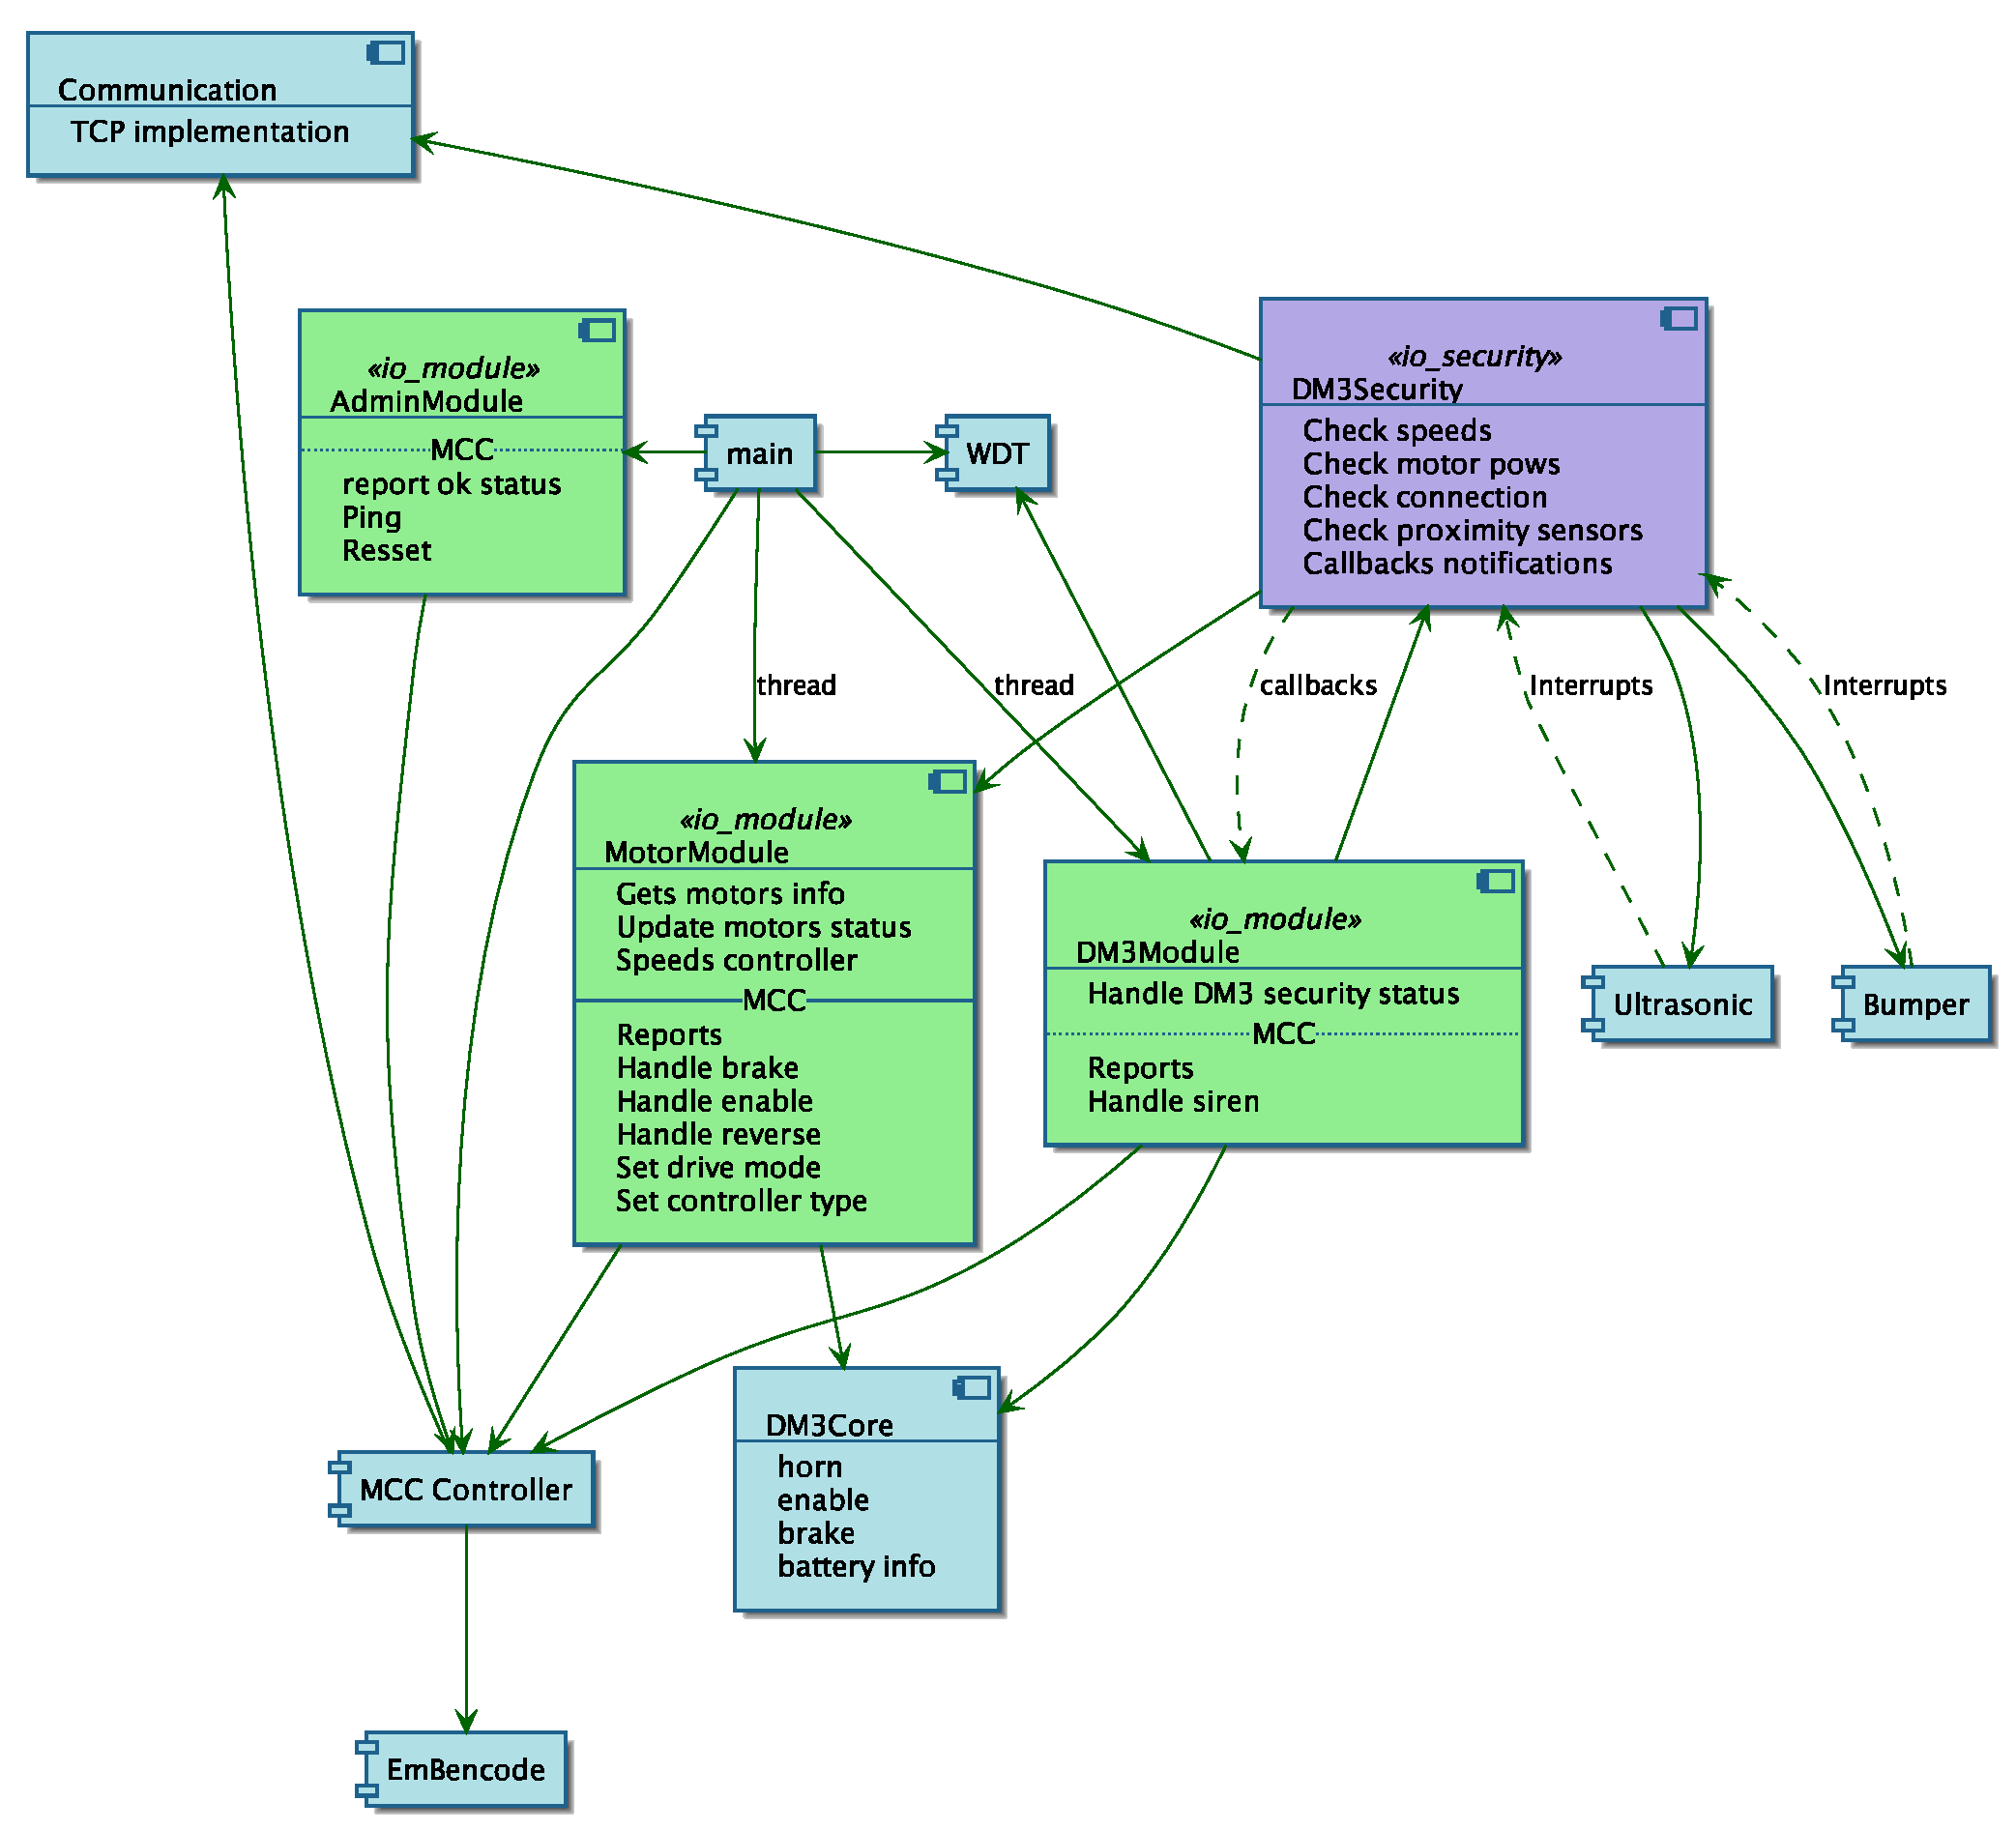
\includegraphics[width=0.8\textwidth]{images/DM3_IOBoard_Components}
\caption[Diagrama de componentes IO Board]{Diagrama de componentes - Firmware IO Board.}
\label{fig: Diagrama de componentes - Firmware IO Board}
\end{figure}

\textbf{mbed ROTS:} El RTOS de mbed no es otra cosa que un envoltorio desarrollado en C++ sobre Keil RTX (\hl{referencia}), que es un RTOS para procesadores ARM y Cortex-M. Provee las funcionalidades que se observan en la Figura \ref{fig: RTX}.

\begin{figure}[H]
  \centering
  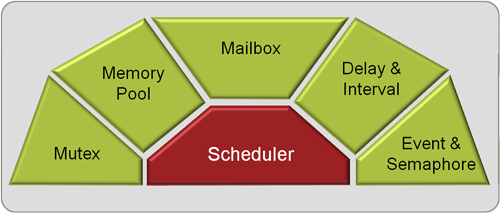
\includegraphics[width=0.5\textwidth]{images/rtx}
  \caption[RTOS - Funcionalidades provistos por RTX]{Funcionalidades provistos por RTX}
  \label{fig: RTX}
\end{figure}

Se utilizo la política de planificación por defecto de RTX, esto es, una política expropiativa con prioridades fijas que frente a tareas con la misma prioridad aplica una política por turnos con un timeslice de \SI{5}{\milli\second}. Adicionalmente, no se asigno prioridades a las diferentes tareas creadas y por esto la política de planificación de nuestra solución es simplemente por turnos.

\paragraph{main}
Programa (hilo) principal, encargado de inicializar al resto de los componentes y de comenzar a procesar los datos provenientes desde la \hl{SBC}. Este hilo principal es quien crea al componente MCC Controller, encargado de recibir información desde la \hl{SBC} y entregarla a los componentes apropiados, así como también instancia otros hilos que procesan y reportan información en los módulos \hl{MotorModule} y \hl{Dm3Module}.

\paragraph{MCC Controller}
Es el componente encargado de implementar el protocolo MCC y de entregar los mensajes a los componentes responsables de su proceso. Cada módulo capaz de intercambiar información con un sistema externo debe registrarse en este controlador siguiendo el protocolo MCC, permitiendo de esta manera que el controlador pueda entregar los mensajes a los componentes apropiados para su procesamiento de forma satisfactoria.

\paragraph{AdminModule}
Componente que al inicializarse se registra en el stack de módulos y operaciones del sistema, siguiendo el protocolo MCC, quedando disponible para procesar solicitudes de ping, reset, o reporte de estado del componente.

\paragraph{MotorModule}
Este componente es responsable de controlar todos los motores del robot, es quién atiende las solicitudes de establecimiento de velocidades a través de mensajes MCC enviados por la \hl{SBC}, procesa dichos mensajes y determina las potencias a establecer en los motores. También es el encargado de generar, y enviar a la \hl{SBC}, reportes de velocidades de las ruedas, potencias y estados de los motores.

\paragraph{Dm3Module} \label{Sol Prop :: Dm3Module}
Componente responsable de manejar el estado general del robot en base a los estados de cada uno de los mecanismos de control de seguridad que se implementan en Dm3Security(\ref{sec:Sol Prop :: Dm3Security}). A continuación se presenta un diagrama de estados en el que se pueden observar los posibles estados del robot y sus transiciones.

\begin{figure}[H]
\centering
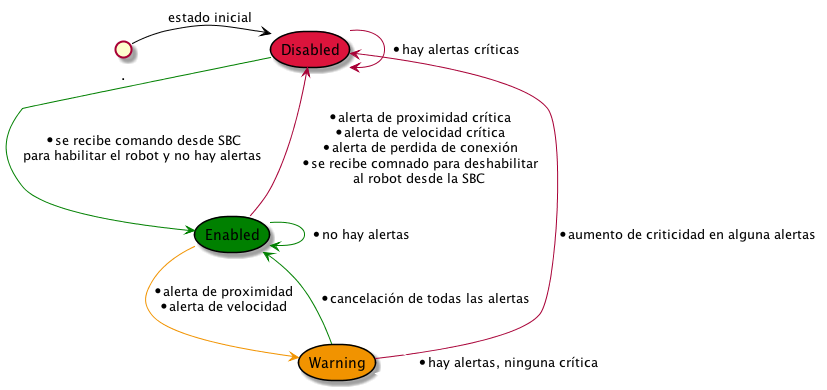
\includegraphics[width=0.8\textwidth]{images/Diagrama_de_estados_del_robot}
\caption[Diagrama de estados del robot]{Diagrama de estados del robot.}
\end{figure}

Se prosigue a describir brevemente las características del robot en cada uno de los estados.
\begin{itemize}
\item \textul{Enabled}: en este estado el robot se encuentra operando o listo para operar con todos sus mecanismos activos y funcionando correctamente. A este estado se puede llegar únicamente cuando se recibe el un comando de habilitación desde la placa \hl{SBC} y el sistema de control de la \hl{IO Board} no ha detectado alertas de seguridad.
\item \textul{Warning}: este estado indica que se ha detectado una alerta de criticidad media, por ejemplo, cuando hay un obstáculo próximo al robot y éste no se está moviendo en dirección a dicho obstáculo, se detecta una alerta de criticidad media por lo que el estado del robot pasa a ser \textit{Warning}. A este estado se llega únicamente desde el estado \textit{Enabled} y es posible pasar al estado \textit{Disabled} en caso de tener una alerta de criticidad mayor, considerando el ejemplo anterior, si se detecta velocidad en dirección al obstáculo el alerta es de criticidad alta.
\item \textul{Disabled}: estado que indica que el robot no está operativo, los motores están deshabilitados y seguramente se encuentre frenado (eventualmente se puede desactivar el freno manualmente aunque el robot esté deshabilitado). Es posible que el robot se encuentre en este estado debido a que se detectó un alerta de criticidad alta como la descrita en el punto anterior o porque se recibió un comando para deshabilitar al robot desde la \hl{SBC}. La única forma de salir de este estado es recibiendo un comando de habilitado desde la \hl{SBC} y que no se detectan alertas de algún tipo, en tal caso el robot pasa al estado \textit{Enabled}.
\end{itemize}

Este componente también es responsable de manejar una sirena, la cual se activa al detectar una alerta de seguridad o al recibir un comando específico para ello desde la \hl{SBC}, y de reportar cada cambio de estado o de alerta de seguridad a la \hl{SBC} mediante mensajes MCC.


\paragraph{Dm3Security} \label{sec:Sol Prop :: Dm3Security}
Es en este componente que se implementan las operaciones de controles relevantes a la seguridad en la operativa del robot. Para ello se siguen dos estrategias, por un lado el monitoreo de componentes utilizado en controles de velocidades \ref{sec:Sol Prop :: detección de velocidades y potencias anómalas} y para la detección y recuperación de la conexión \ref{sec:Sol Prop :: monitoreo y recuperación de la conexión}; por otra parte se empleó un manejo de interrupciones en la detección de objetos próximo \ref{sec:Sol Prop :: detección de objetos próximos}.
El componente provee un mecanismo de registro para ser notificado con el estado de cada uno de los mecanismos de seguridad implementados. Actualmente el Dm3Module (\ref{Sol Prop :: Dm3Module}) es el único componente que se suscribe a dichas notificaciones y en base a ellas toma acciones de seguridad generando reportes que son enviados a la \hl{SBC}.

\section{Protocolo de Comunicación}
El protocolo de comunicación central y sobre el que se implementa la comunicación entre los componentes y sistemas del robot es MCC (\ref{sec: Marco Teo :: MCC}). En la comunicación entre sistemas \hl{IO Board} y \hl{SBC} se utiliza el protocolo TCP mediante un \hl{soket} que conecta ambos sistemas.

En los inicios del proyecto se evaluó el uso del protocolo \hl{HDLC} sobre un \hl{enlace serial USB} y no sólo se investigó sobre el protocolo sino que se implementó una versión (básica) del mismo, pero debido a la complejidad que presentó llevar dicha implementación al hardware del aplaca IO Board, que también se estaba evaluando en ese momento, optamos por cambiar el hardware para la IO Board y consigo el protocolo de comunicación con la \hl{SBC}. Esto fue debido a que el nuevo hardware contempla un módulo que permite establecer una \hl{conexion Ethernet} mediante un \hl{conector RJ45}, lo que nos entusiasmó a utilizar un protocolo ya implementado \hl{por la comunidad} y maduro como lo es TCP en lugar de nuestra implementación del protocolo HDLC.
Algunas de las ventajas del uso de TCP frente al uso de HDLC:
\begin{itemize}
\item El protocolo ya se encuentra implementado en las diferentes tecnologías de cada sistema, por la comunidad de desarrolladores \hl{mbed} en el caso de la IO Board y por \hl{GNU Projects} en el caso de la \hl{SBC}. En cualquiera de los casos son implementaciones maduras que ofrecen garantías de calidad.
\item TCP garantiza que los paquetes serán recibidos en el orden correcto y la implementación básica que se desarrolló de HDLC no contaba con esta característica.
\item El rendimiento que obtuvimos con la comunicación TCP en la transferencia exitosa de datos fue considerablemente mejor que el obtenido utilizando HDLC. \hl{REVISAR ESTA AFIRMACION}
\item Otra característica que pone en ventaja al uso de TCP es la flexibilidad y facilidad para poder establecer múltiples conexiones entre los sistemas, por ejemplos para el caso en el que se quisiera tener una conexión específica para un módulo o componente.
\end{itemize}

\section{Supervisión de Sub-sistemas y componentes}
Como se mencionó en la sección \ref{sec:Sol Prop :: Dm3Security} el componente Dm3Security es el responsable de monitorear al resto de los componentes  y atender las rutinas de interrupción que generan alertas de seguridad en lo que respecta al correcto comportamiento del robot en un escenario de trabajo colaborativo con humanos. A pesar de tener este comportamiento resuelto en el componente \hl{Dm3Security} es necesario proveer un mecanismo de control sobre el propio componente, un mecanismo incluso más general que garantice que el propio sistema de control está ejecutando correctamente y en caso contrario tome acciones para restaurar su funcionamiento.
Para proveer tales características se propone el uso del componente Watchdog que se describe a continuación en la sección  \ref{sec: Sol Prop :: Watchdog}.

\subsection{Watchdog} \label{sec: Sol Prop :: Watchdog}
El componente Watchdog no es más que un manejador de un temporizador de vigilancia \hl{(Watch Dog Timer)}, un temporizador de hardware que genera automáticamente un restablecimiento del sistema si el programa principal deja de atenderlo con cierta frecuencia. Es un componente sumamente importante para  restablecer automáticamente al sistema de control del robot si este se cuelga debido a un error de software o hardware. Nuestra IO Board tiene hardware de temporizador de vigilancia que nos permite implementar el componente Watchdog mencionado.

El programa principal de la \hl{IO Board} tiene un bucles que constantemente realiza diversas funciones, el temporizador de vigilancia se carga con un valor inicial mayor que el peor tiempo procesamiento que pude tomar realizar dichas funciones de los bucles. Cada vez que se cierra un ciclo de procesamiento se restablece el temporizador de vigilancia. Si ocurre una falla y el programa principal no regresa para restablecer el temporizador antes de que expire el tiempo establecido, se genera una interrupción para restablecer el procesador y con ello al sistema de control.
Cabe mencionar que el componente Dm3Security (\ref{sec:Sol Prop :: Dm3Security}) genera un reporte de estados en el que se indica si el sistema fue reiniciado por el temporizador de vigilancia o si inició debido a un encendido normal del sistema.

Consideramos que es sumamente importante la implementación de éstos componentes en sistemas autónomos como lo es en el caso del robot Dm3. Para ejemplificar y mostrar la importancia que tiene les contaremos sobre un caso de la vida real:

\textit{En un famoso caso \cite{Clementine}, una computadora de la sonda espacial de la NASA se bloqueó con los cohetes propulsores encendidos. Para el momento en el que los controladores presentes en la tierra se dieron cuenta del problema y enviaron una señal para forzar el reinicio del hardware de la sonda, ésta había utilizado todo su combustible. El procesador de la sonda tenía un temporizador de vigilancia pero no fue utilizado, de haberlo hecho probablemente habría detectado la falla y apagaría los motores del cohete a tiempo para salvar la misión.}

\subsection{Detección de Objetos Próximos} \label{sec:Sol Prop :: detección de objetos próximos}
Si bien el robot cuenta con un sistema de navegación y detección de obstáculos implementado en la \hl{SBC} creemos necesario implementar en la \hl{IO Board} otros mecanismos para la detección de objetos próximos que estén controlados por el componente Dm3Security (\ref{sec:Sol Prop :: Dm3Security}). Se utilizará para ello un conjunto de sensores de distancia que permitirán detectar la presencia de objetos a distancias cercanas a los cuatro metros. 

También es necesario considerar que todos los mecanismos de detección de objetos próximos han fallado y se presenta el accidente o colisión, es muy importante poder detectar este caso y tomar acciones de forma muy eficiente. Para ello se utilizan sensores contacto \hl{Bumpers} que alerten de una colisión en tiempo real generando una interrupción en el sistema para que el componente Dm3Security (\ref{sec:Sol Prop :: Dm3Security}) procese la información y tome las acciones correspondientes (apagar los motores, activar frenos, encender una sirena, etc.).

\subsection{Detección de Velocidades y Potencias Anómalas} \label{sec:Sol Prop :: detección de velocidades y potencias anómalas}
Debemos garantizar que el robot se moverá en un rango de velocidades bien establecido, para ello se implementan mecanismos de control en el componente Dm3Security (\ref{sec:Sol Prop :: Dm3Security}) que monitorean las velocidades de las ruedas del robot y validan que estén dentro de los parámetros configurados, de no estarlo se ejecutan rutinas que de seguridad que eventualmente deshabilitan al robot y reportan el estado de los componentes a los operarios.
Además de los controles de velocidades propiamente, se definen controles que relacionan la velocidad del robot con la potencia establecida en los motores. Estos controles monitorean las velocidades y las potencias verificando que la diferencia, en términos porcentuales, entre velocidad y potencia no supere a un valor configurado. Con este mecanismo se pretende detectar escenarios en los que el robot se encuentra realizando una sobrecarga de los motores, ya sea porque se encuentra en una pendiente demasiado pronunciada y transporta una gran carga de peso o simplemente porque tiene una rueda atascada en una irregularidad de suelo.
Al detectar cualquiera de los escenarios mencionados anteriormente el robot será deshabilitado y se reportará a los operarios de lo sucedido.

\subsection{Monitoreo y Recuperación de la Conexión} \label{sec:Sol Prop :: monitoreo y recuperación de la conexión}
Se proporciona un mecanismo que monitorea la conexión entre la \hl{SBC} y la \hl{IOBoard} y en caso de detectar una pérdida de ésta genera una alerta crítica de seguridad que concluye en deshabilitar al robot. También se implementa un mecanismo que intenta restablecer la conexión una vez que se detecta la pérdida de la misma. Este mecanismo es totalmente independiente del que tomas las acciones para deshabilitar al robot.

\section{Indicadores de Estado} \label{sec: sol prop - Indicadores de Estado}
El robot cuenta con dispositivos que permiten indicar a los operarios sobre el estado del robot y el funcionamiento de sus componentes. Estos dispositivos son:
\begin{itemize}
\item Pantalla LCD informando el estado general del robot y el reporte de los mecanismos de seguridad mencionados en las secciones anteriores.
\item Sirena audible que se activa frente a una alerta de seguridad, ya sea de criticidad baja como puede ser el haber detectado un objeto próximo pero el robot no se está moviendo en dirección al objeto, como también una vez que el robot fue deshabilitado a consecuencia de un alerta de seguridad.
\item Luz de emergencia que indica que el robot está con alimentación de energía y que eventualmente puede estar en movimiento.
\end{itemize}

\chapter{Implementación}
En este capítulo se describe la implementación de lo descrito en el capítulo anterior, Solución Propuesta. En la sección \ref{sec: Implementación :: Plataforma Utilizada} se describe la plataforma de hardware utilizada, luego, en la sección \ref{sec: Implementación :: Supervisión} se describe la implementación del modulo de supervisión de sub-sistemas y componentes y, finalmente, en la sección \ref{sec: Implementación :: Indicadores de Estado} se presenta la implementación de los mecanismos para indicar estados del robot a operarios.

\section{Plataforma Utilizada} \label{sec: Implementación :: Plataforma Utilizada}
\subsection{Prototipo DM3}
El robot DM3 con el cual se trabajo en este proyecto es un prototipo de robot para la agricultura cuyo propósito es, como se menciona en \ref{sec: Introduccion :: Motivacion}, el de asistir en la cosecha de peras y manzanas, liberando así tiempo de los trabajadores que es actualmente utilizado en el transporte de las frutas para que puedan concentrarse en la recolección en si. En las Figuras \ref{fig:PrototipoDM31}, \ref{fig:PrototipoDM32} y \ref{fig:PrototipoDM33} se puede observar el prototipo construido y ver hardware el que lo compone enumerado.

\begin{figure}[H]
  \centering
  \begin{minipage}[b]{0.49\textwidth}
    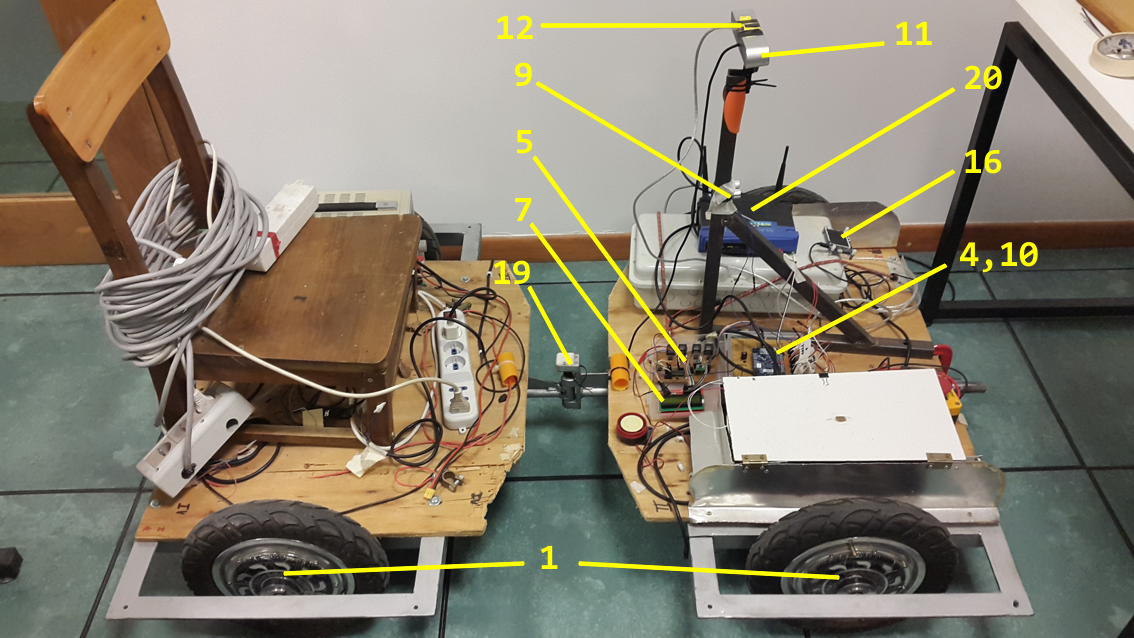
\includegraphics[width=\textwidth]{images/Robot1}
    \caption[Prototipo DM3, vista lateral derecha.]{Prototipo DM3, vista lateral derecha.}
    \label{fig:PrototipoDM31}
  \end{minipage}
  \hfill
  \begin{minipage}[b]{0.49\textwidth}
    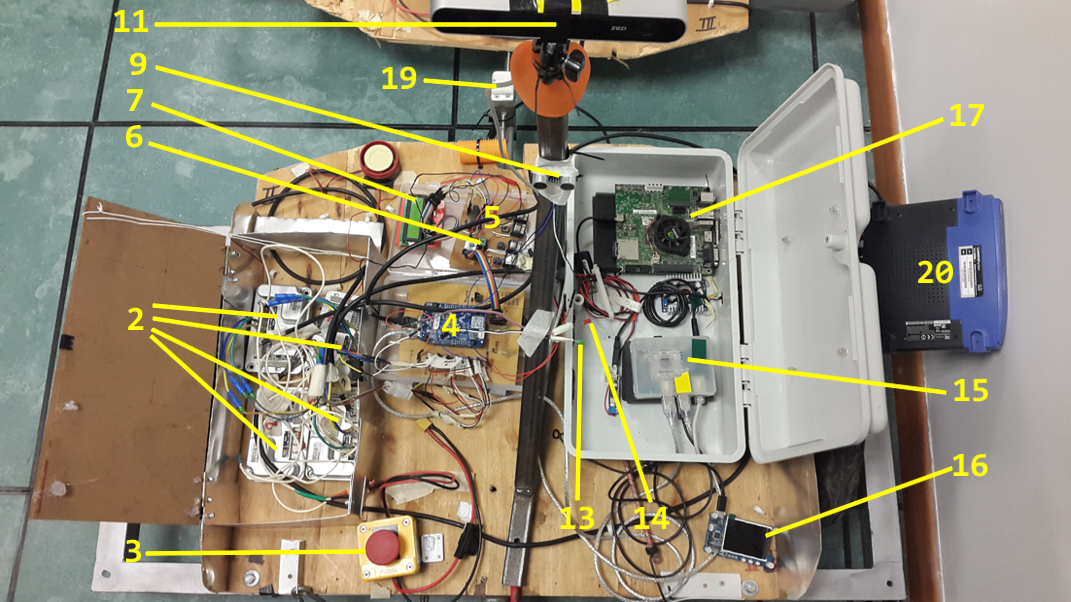
\includegraphics[width=\textwidth]{images/Robot2}
    \caption[Prototipo DM3, chasis 0, vista anterior]{Prototipo DM3, chasis 0, vista anterior}
    \label{fig:PrototipoDM32}
  \end{minipage}
\end{figure}

\begin{figure}[H]
  \centering
  \begin{minipage}[b]{0.49\textwidth}
    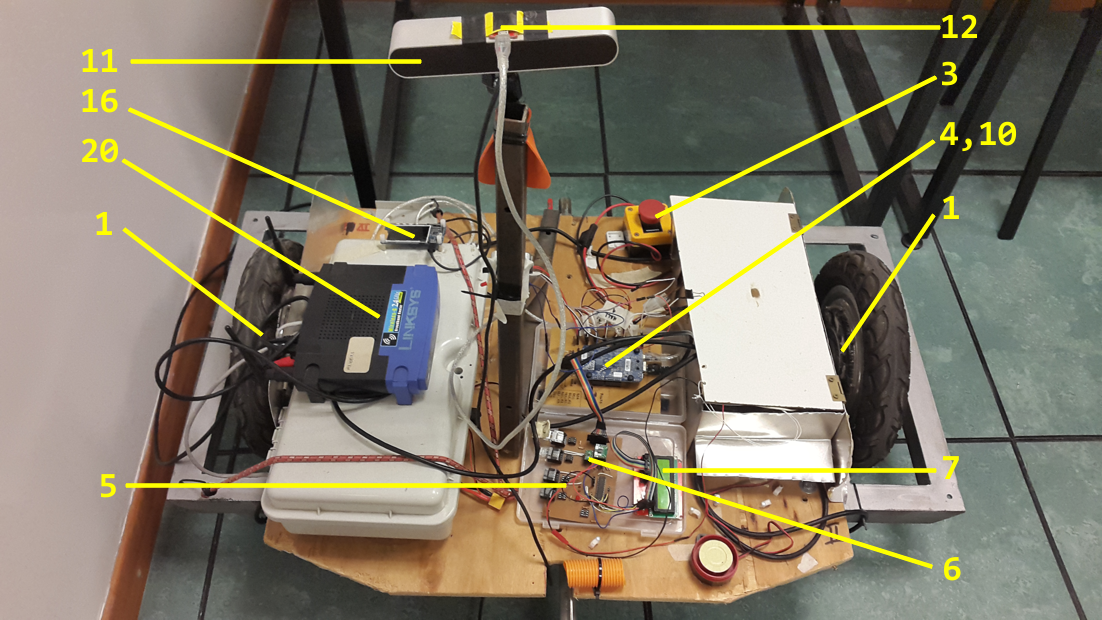
\includegraphics[width=\textwidth]{images/Robot3}
    \caption[Prototipo DM3, chasis 0, vista posterior]{Prototipo DM3, chasis 0, vista posterior}
    \label{fig:PrototipoDM33}
  \end{minipage}
\end{figure}

Los números que figuran en las imágenes se corresponden con los siguientes componentes:
\begin{enumerate}[noitemsep]
  \item Motores
  \item Controladoras de motores
  \item Botón de parada de emergencia
  \item Placa de Entrada/Salida conectada a \textit{shield} construido para ella.
  \item Shield octocoplado para \hl{DAC}
  \item DAC
  \item LCD de estado de los motores \cite{LCD1602}
  \item Módulo \hl{GPS} con interfaz \hl{USB} \cite{GPSModule}
  \item Sensor de distancia ultrasonido
  \item Sensor de contacto
  \item Cámara 3D (ZED)
  \item Sensor inercial \cite{myAHRS}
  \item Sirena (LED verde)
  \item Freno (LED Rojo)
  \item SBC ROS
  \item Display LCD
  \item SBC ZED
  \item Batería
  \item Encoder de la articulación entre los chasis (\hl{MODELO?})
  \item Router
\end{enumerate}

Se incluye por completitud los ítems 8 y 18, módulo GPS y batería respectivamente. El módulo GPS quedó oculto bajo la caja que contiene las SBC y la batería no estaba instalada al momento de tomar las fotografías.

\subsection{Detalle del Hardware} \label{sec: Implementación :: Plataforma Utilizada - Hardware}
Se expone a continuación los componentes de hardware mas relevantes al proyecto incluidos en el prototipo.

\subsubsection{Placas de Computo} 
La placa de entrada/salida en la cual se concentro la mayor parte del software construido en el contexto del proyecto es la FRDM K64F, ítem 4 de las Figuras \ref{fig:PrototipoDM31}, \ref{fig:PrototipoDM32} y \ref{fig:PrototipoDM33}. Se puede encontrar un análisis minucioso de la misma en la sección 4.4 de \cite{RASSOA}. Cabe destacar que al inicio del proyecto se trabajo con otra placa de entrada/salida, la Odroid USB IO Board (se puede encontrar detalle de la misma en \cite{RASSOA}), que luego se descarto debido a cambios en los requerimientos que la placa no logro satisfacer (capacidades de expansión) y que se decidió apostar por una placa mas moderna con hardware mas poderoso, siendo finalmente seleccionada la que tiene las mayores capacidades de hardware y de expansión de entre las analizadas, ver sección 4.8 de \cite{RASSOA}.

La SBC utilizada, ítem 15 de las Figura \ref{fig:PrototipoDM32}, para ejecutar la mayoría de las funciones de alto nivel es la Odroid XU3 Lite, en \cite{ODROIDXU3} se encuentra una descripción detallada de la placa. Esta placa es la encargada de ejecutar ROS y los nodos ROS implementados.

El ítem 17 de la Figura \ref{fig:PrototipoDM32} corresponde a la SBC Jetson TK1 de NVIDIA \cite{TegraTk1}. Si bien esta placa no atañe al proyecto se la presenta pues es la encargada de procesar la información capturada por la cámara 3D, ZED, de la empresa Stereolabs. Valiéndose de un empaquetado (\textit{wrapper}) para el SDK del ZED, provisto por Stereolabs, el resultado del procesamiento de la información capturada por el ZED se comunica a los nodos ROS ejecutando en la Odroid XU3 Lite.

La placa Odroid SHOW 2 es una placa de entrada/salida compatible con Arduino que se utilizo como display indicador de los estados del prototipo, ítem 16 de las Figuras \ref{fig:PrototipoDM31}, \ref{fig:PrototipoDM32} y \ref{fig:PrototipoDM33}. En la sección 4.7 de \cite{RASSOA} se puede observar sus características en detalle, como allí se observa esta placa tiene reducidas capacidades de expansión y poder de computo, razón por la cual solo se utilizo su pantalla LCD.

\subsubsection{\textit{Shield} para Placa de Entrada/Salida}
A los efectos de facilitar la integración de la placa de entrada/salida al prototipo, contar con conexiones mas seguras y fáciles de intercambiar, se diseño y construyo un \textit{shield} para la placa FRDM K64F en el cual se exponen de forma organizada los pines de extensión utilizados. En las Figuras \ref{fig:ShieldFront}, \ref{fig:ShieldBack} y \ref{fig:ShieldSchematic} se puede observar el \textit{shield} construido con la placa de entrada/salida colocada, el \textit{shield} solo y el diseño esquemático del mismo respectivamente.

\begin{figure}[H]
  \centering
  \begin{minipage}[t]{0.4\textwidth}
    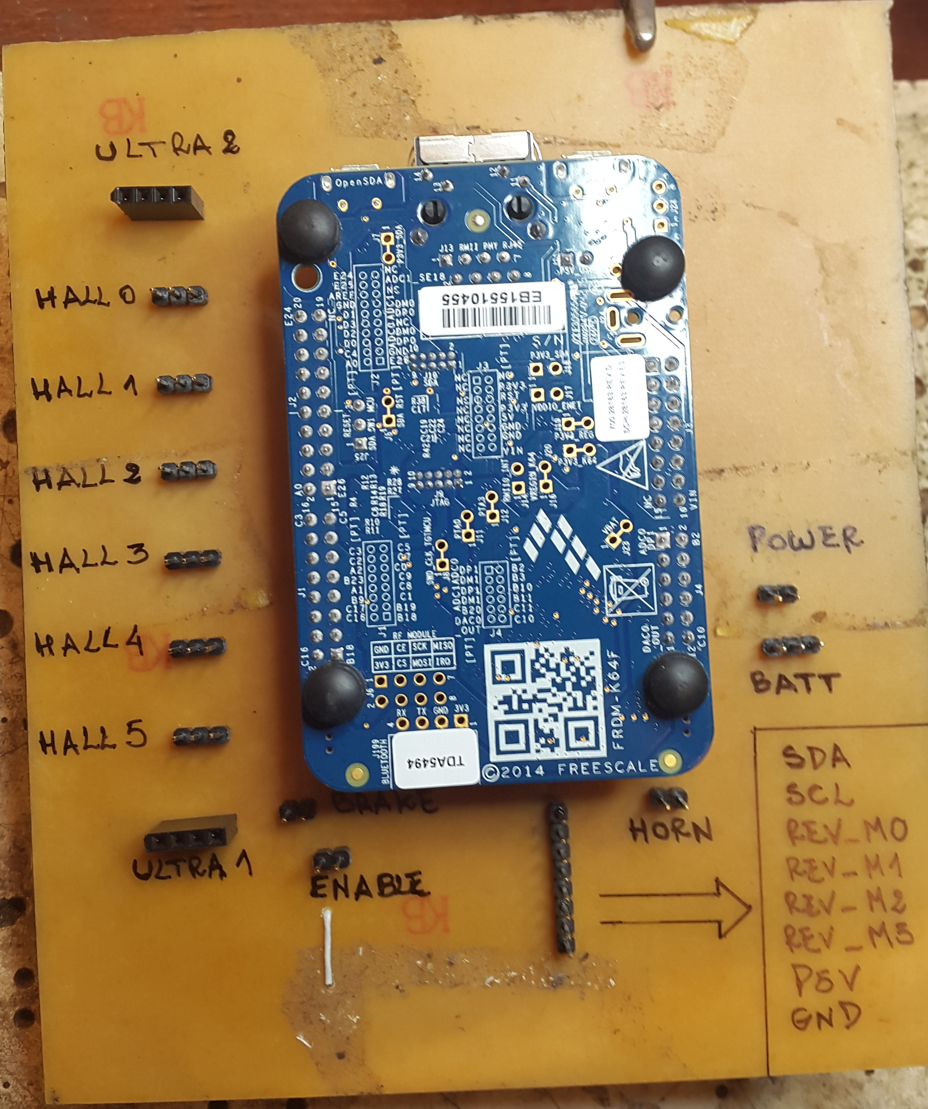
\includegraphics[width=\textwidth]{images/Shield_K64F}
    \caption[Shield, vista frontal]{Shield, vista frontal con placa de entrada/salida FRDM K64F colocada.}
    \label{fig:ShieldFront}
  \end{minipage}
  \hfill
  \begin{minipage}[t]{0.4\textwidth}
    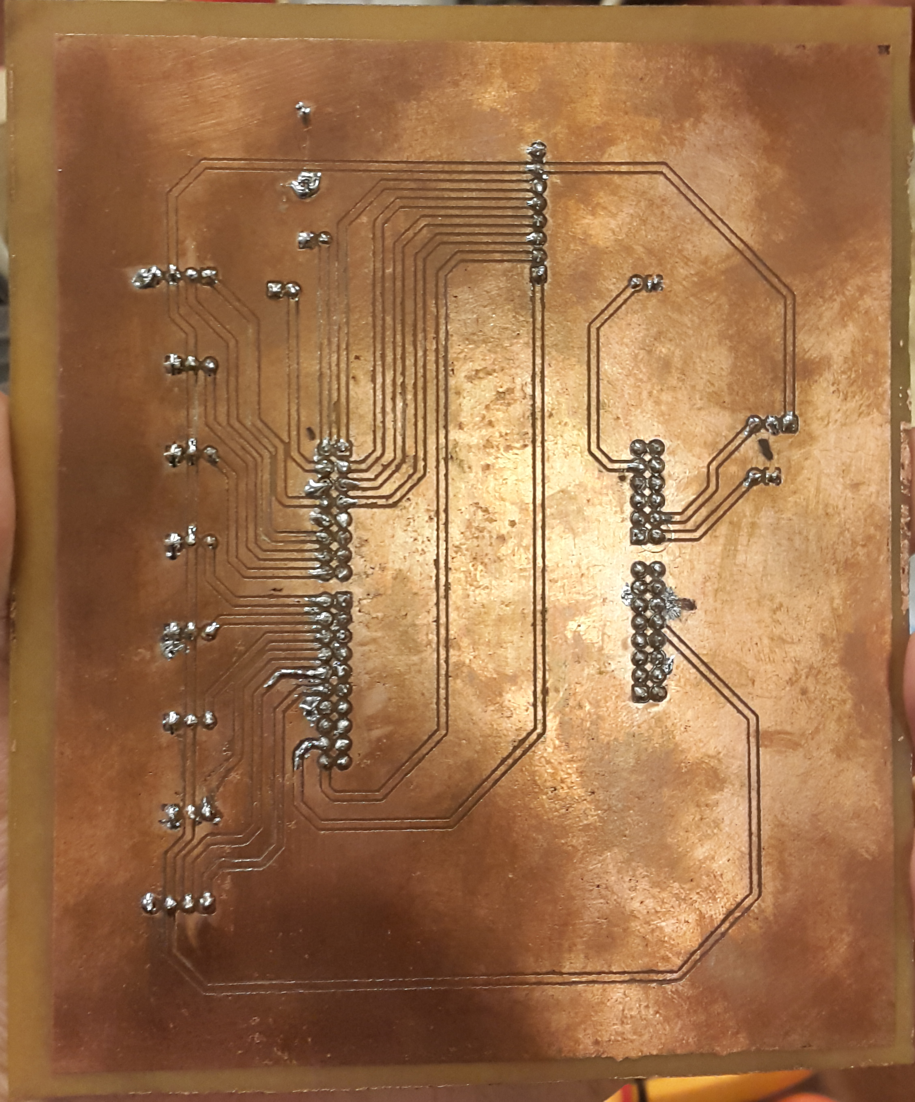
\includegraphics[width=\textwidth]{images/Shield_Back}
    \caption[Shield, vista trasera]{Shield, vista trasera.}
    \label{fig:ShieldBack}
  \end{minipage}
\end{figure}

\begin{figure}[H]
  \centering
  \begin{minipage}[b]{0.49\textwidth}
    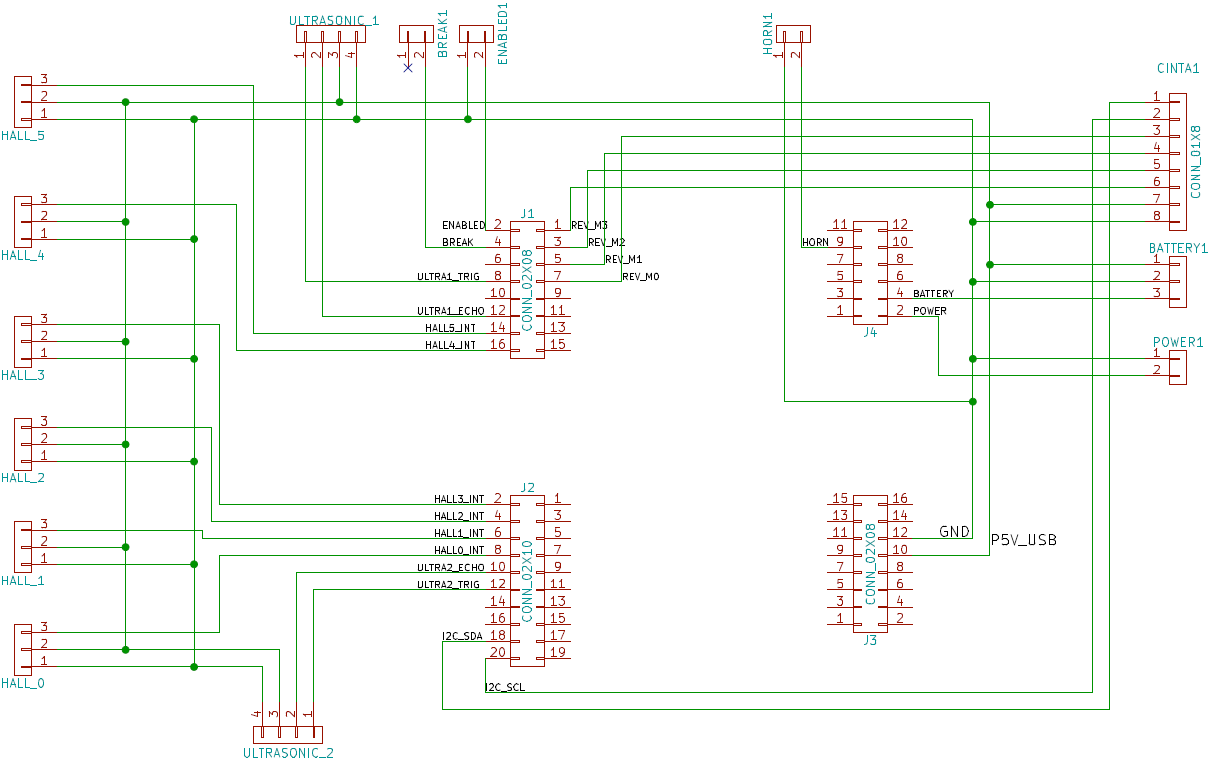
\includegraphics[width=\textwidth]{images/Shield_Schematic}
    \caption[Diseño esquemático del shield]{Diseño esquemático del shield.}
    \label{fig:ShieldSchematic}
  \end{minipage}
\end{figure}

\subsubsection{Sensores}
El sensor de distancia de ultrasonido utilizado, ítem 9 de las Figuras \ref{fig:PrototipoDM31} y \ref{fig:PrototipoDM32}, es el HC-SR04 cuyo funcionamiento y características se puede observar en \cite{HCSR04}.

El kill switch utilizado es el que se observa en las Figuras \ref{fig:PrototipoDM32} y \ref{fig:PrototipoDM33}, ítem 3.

A los efectos de implementar el mecanismo de detección con sensores de contacto, ver \ref{sec:Implementacion :: detección de objetos próximos :: Contacto}, se utilizó un botón de los disponibles en la placa de entrada/salida (Figuras \ref{fig:PrototipoDM31} y \ref{fig:PrototipoDM33}, ítem 4).

\subsubsection{Actuadores} \label{sec: Implementación :: Plataforma Utilizada - Hardware - Actuadores}
Los ítems 1 y 2 de las Figuras \ref{fig:PrototipoDM31}, \ref{fig:PrototipoDM32} y \ref{fig:PrototipoDM33} corresponden a los motores y las placas controladoras de los mismos respectivamente. Los motores son los Magic Pie 3 de Golden Motors, en \cite{MagicPie3} se puede ver su información detallada, y las controladoras son las Magic Controller V2 cuyo detalle se puede ver en \cite{MagicControllerV2}. Es de las controladoras Magic Controller V2 que se obtienen las lecturas de los sensores de hall de los motores.

El prototipo no incluyó una sirena y freno instalados, a los efectos de experimentar con los mecanismos de seguridad asociados a estos componentes (que se activan/desactivan) se utilizaron dos LED, uno verde (ítem 13 de la Figura \ref{fig:PrototipoDM32}) para representar la sirena y uno rojo (ítem 14 de la Figura \ref{fig:PrototipoDM32}) para representar el freno.

\subsubsection{Otros} \label{sec: Implementación :: Plataforma Utilizada - Hardware - Otros}
Como se comentó en \ref{sec:Sol Prop :: Requerimientos} cuando se describieron los requerimientos de hardware, se utilizó un DAC para dar potencia a los motores, el modelo del mismo es MPC4728 y se pueden observar sus características en \cite{MPC4728}. Es el ítem 6 de las Figuras \ref{fig:PrototipoDM32} y \ref{fig:PrototipoDM33}.

\subsection{Entorno de desarrollo}
\begin{itemize}
    \item IDEs
    \item Librerías y SDKs
    \item Repositorios de código
\end{itemize}
\section{Supervisión de Sub-sistemas y componentes} \label{sec: Implementación :: Supervisión}
Para dar un panorama general de los componentes del sistema de control y sus relaciones, se presenta el siguiente diagrama.

\begin{figure}[H]
\centering
\label{fig: Diagrama_de_subsistema_Dm3Security}
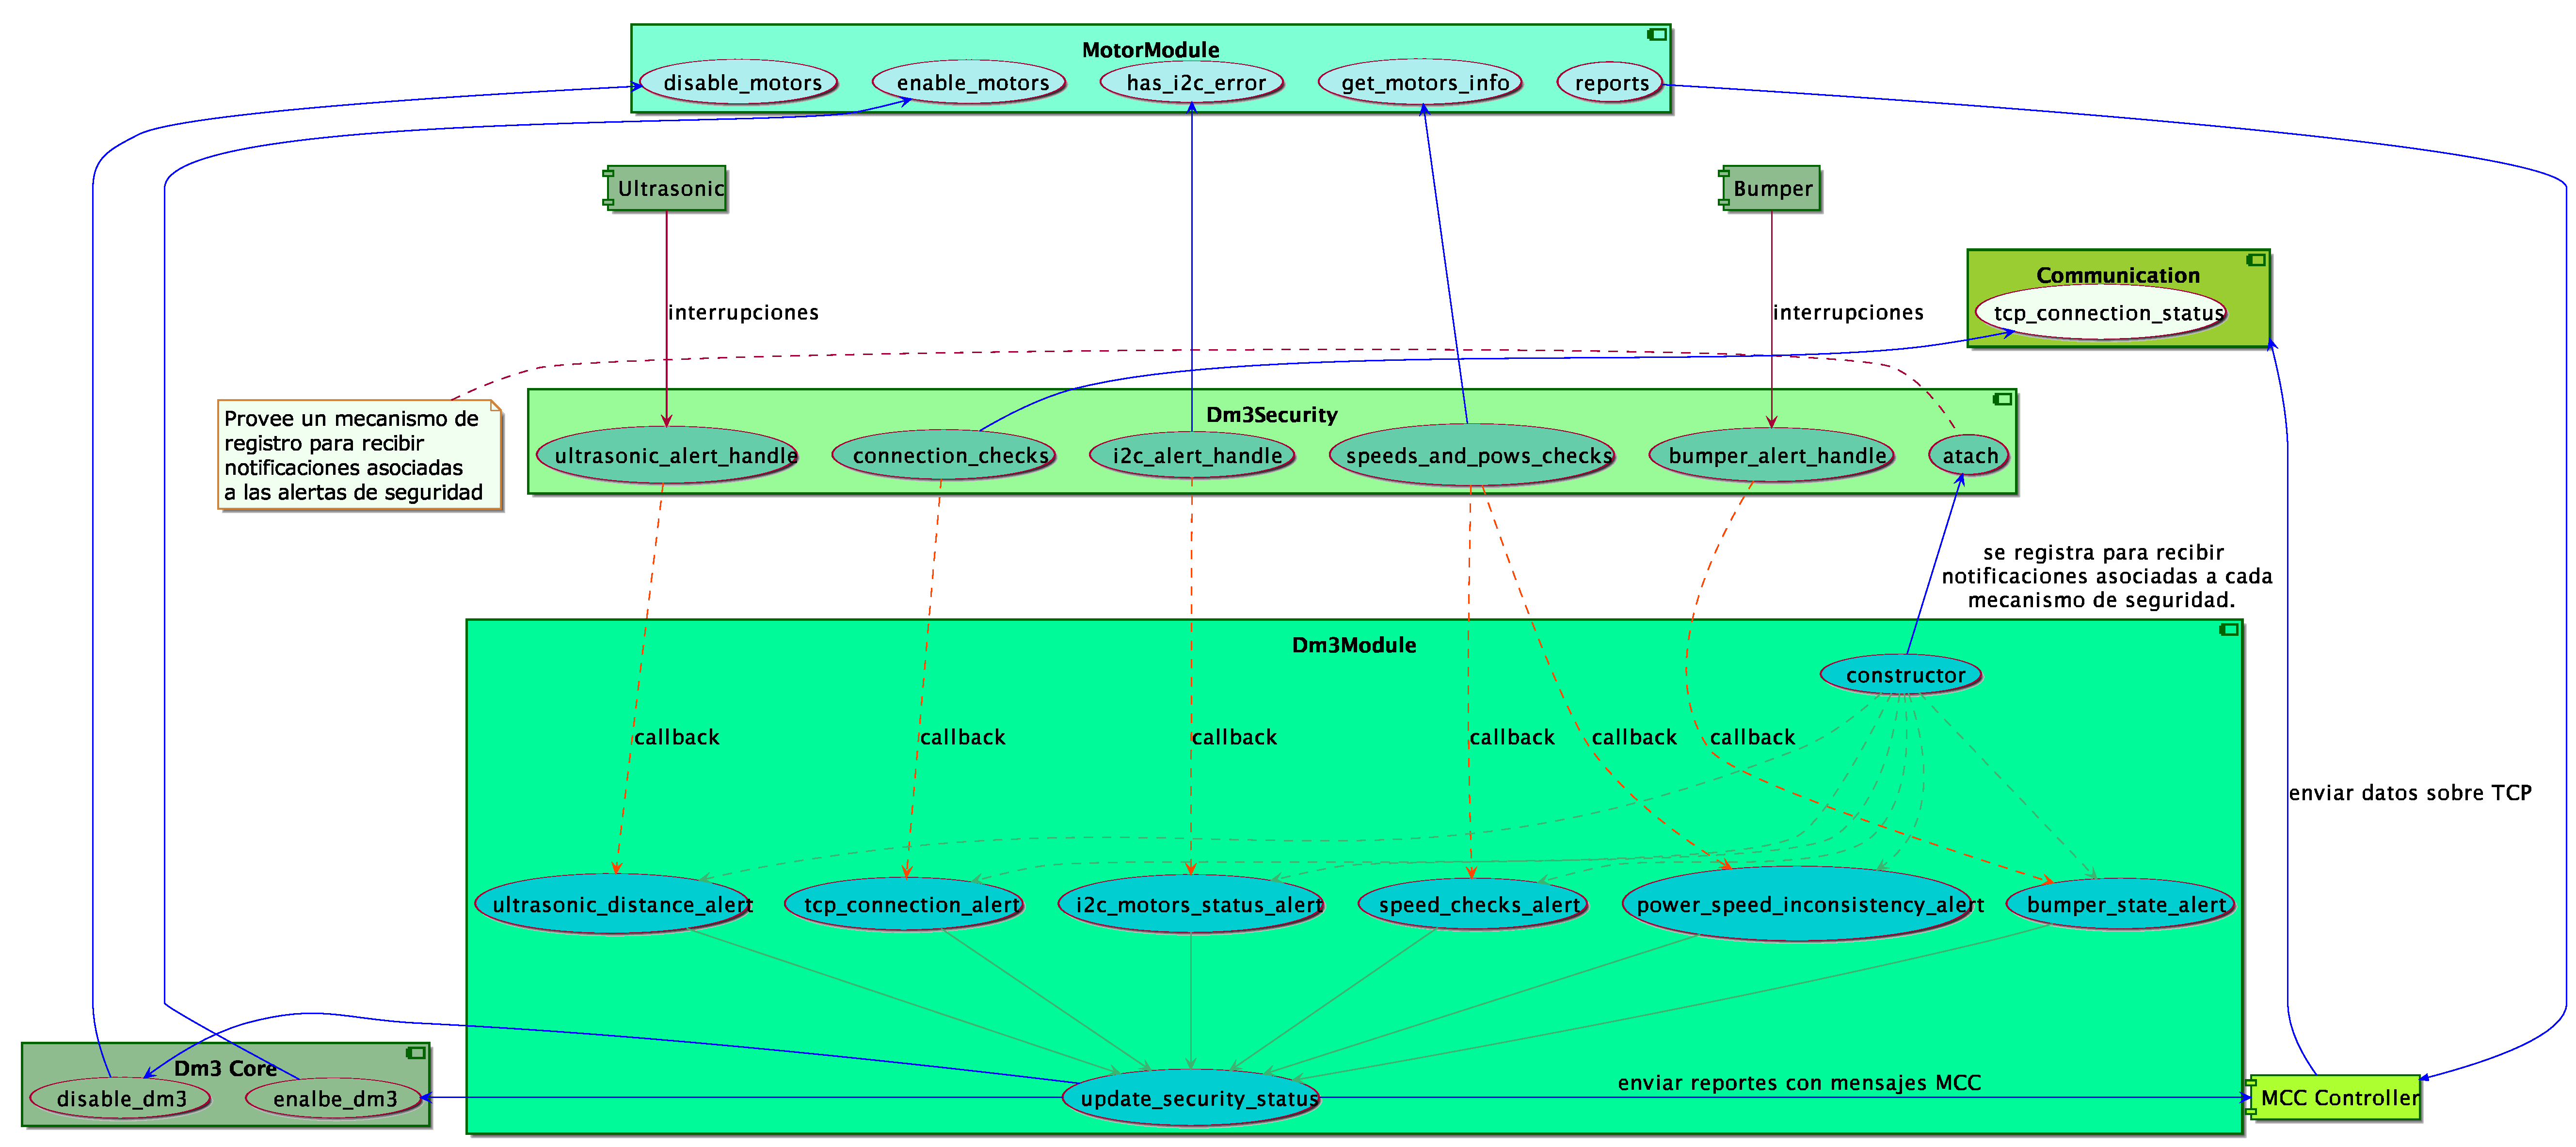
\includegraphics[width=\textwidth]{images/Diagrama_de_subsistema_Dm3Security}
\caption[Diagrama del sub-sistema Dm3Security]{Diagrama de relación de componentes del sistema de control.}
\end{figure}

El componente Dm3Security define un conjunto de mecanismos para realizar chequeos de seguridad, así como también provee un mecanismo de suscripción para recibir alertas o notificaciones generadas por dichos mecanismos. Se puede observar en el diagrama de la figura \ref{fig: Diagrama_de_subsistema_Dm3Security} que el componente Dm3Module es quien se subscribe para recibir las notificaciones y de esta manera tomar las acciones correspondientes, entre las que se encuentran: (des)habilitar al robot, activar alertas audibles y visibles, frenar las ruedas, generar y enviar reportes a la \hl{SBC}.
El siguiente diagrama describe el flujo del proceso implementado para procesar las alertas de seguridad y manejar los estados del robot.

\begin{figure}[H]
\centering
\label{fig: Diagrama_de_flujo_proceso_alertas_de_seguridad}
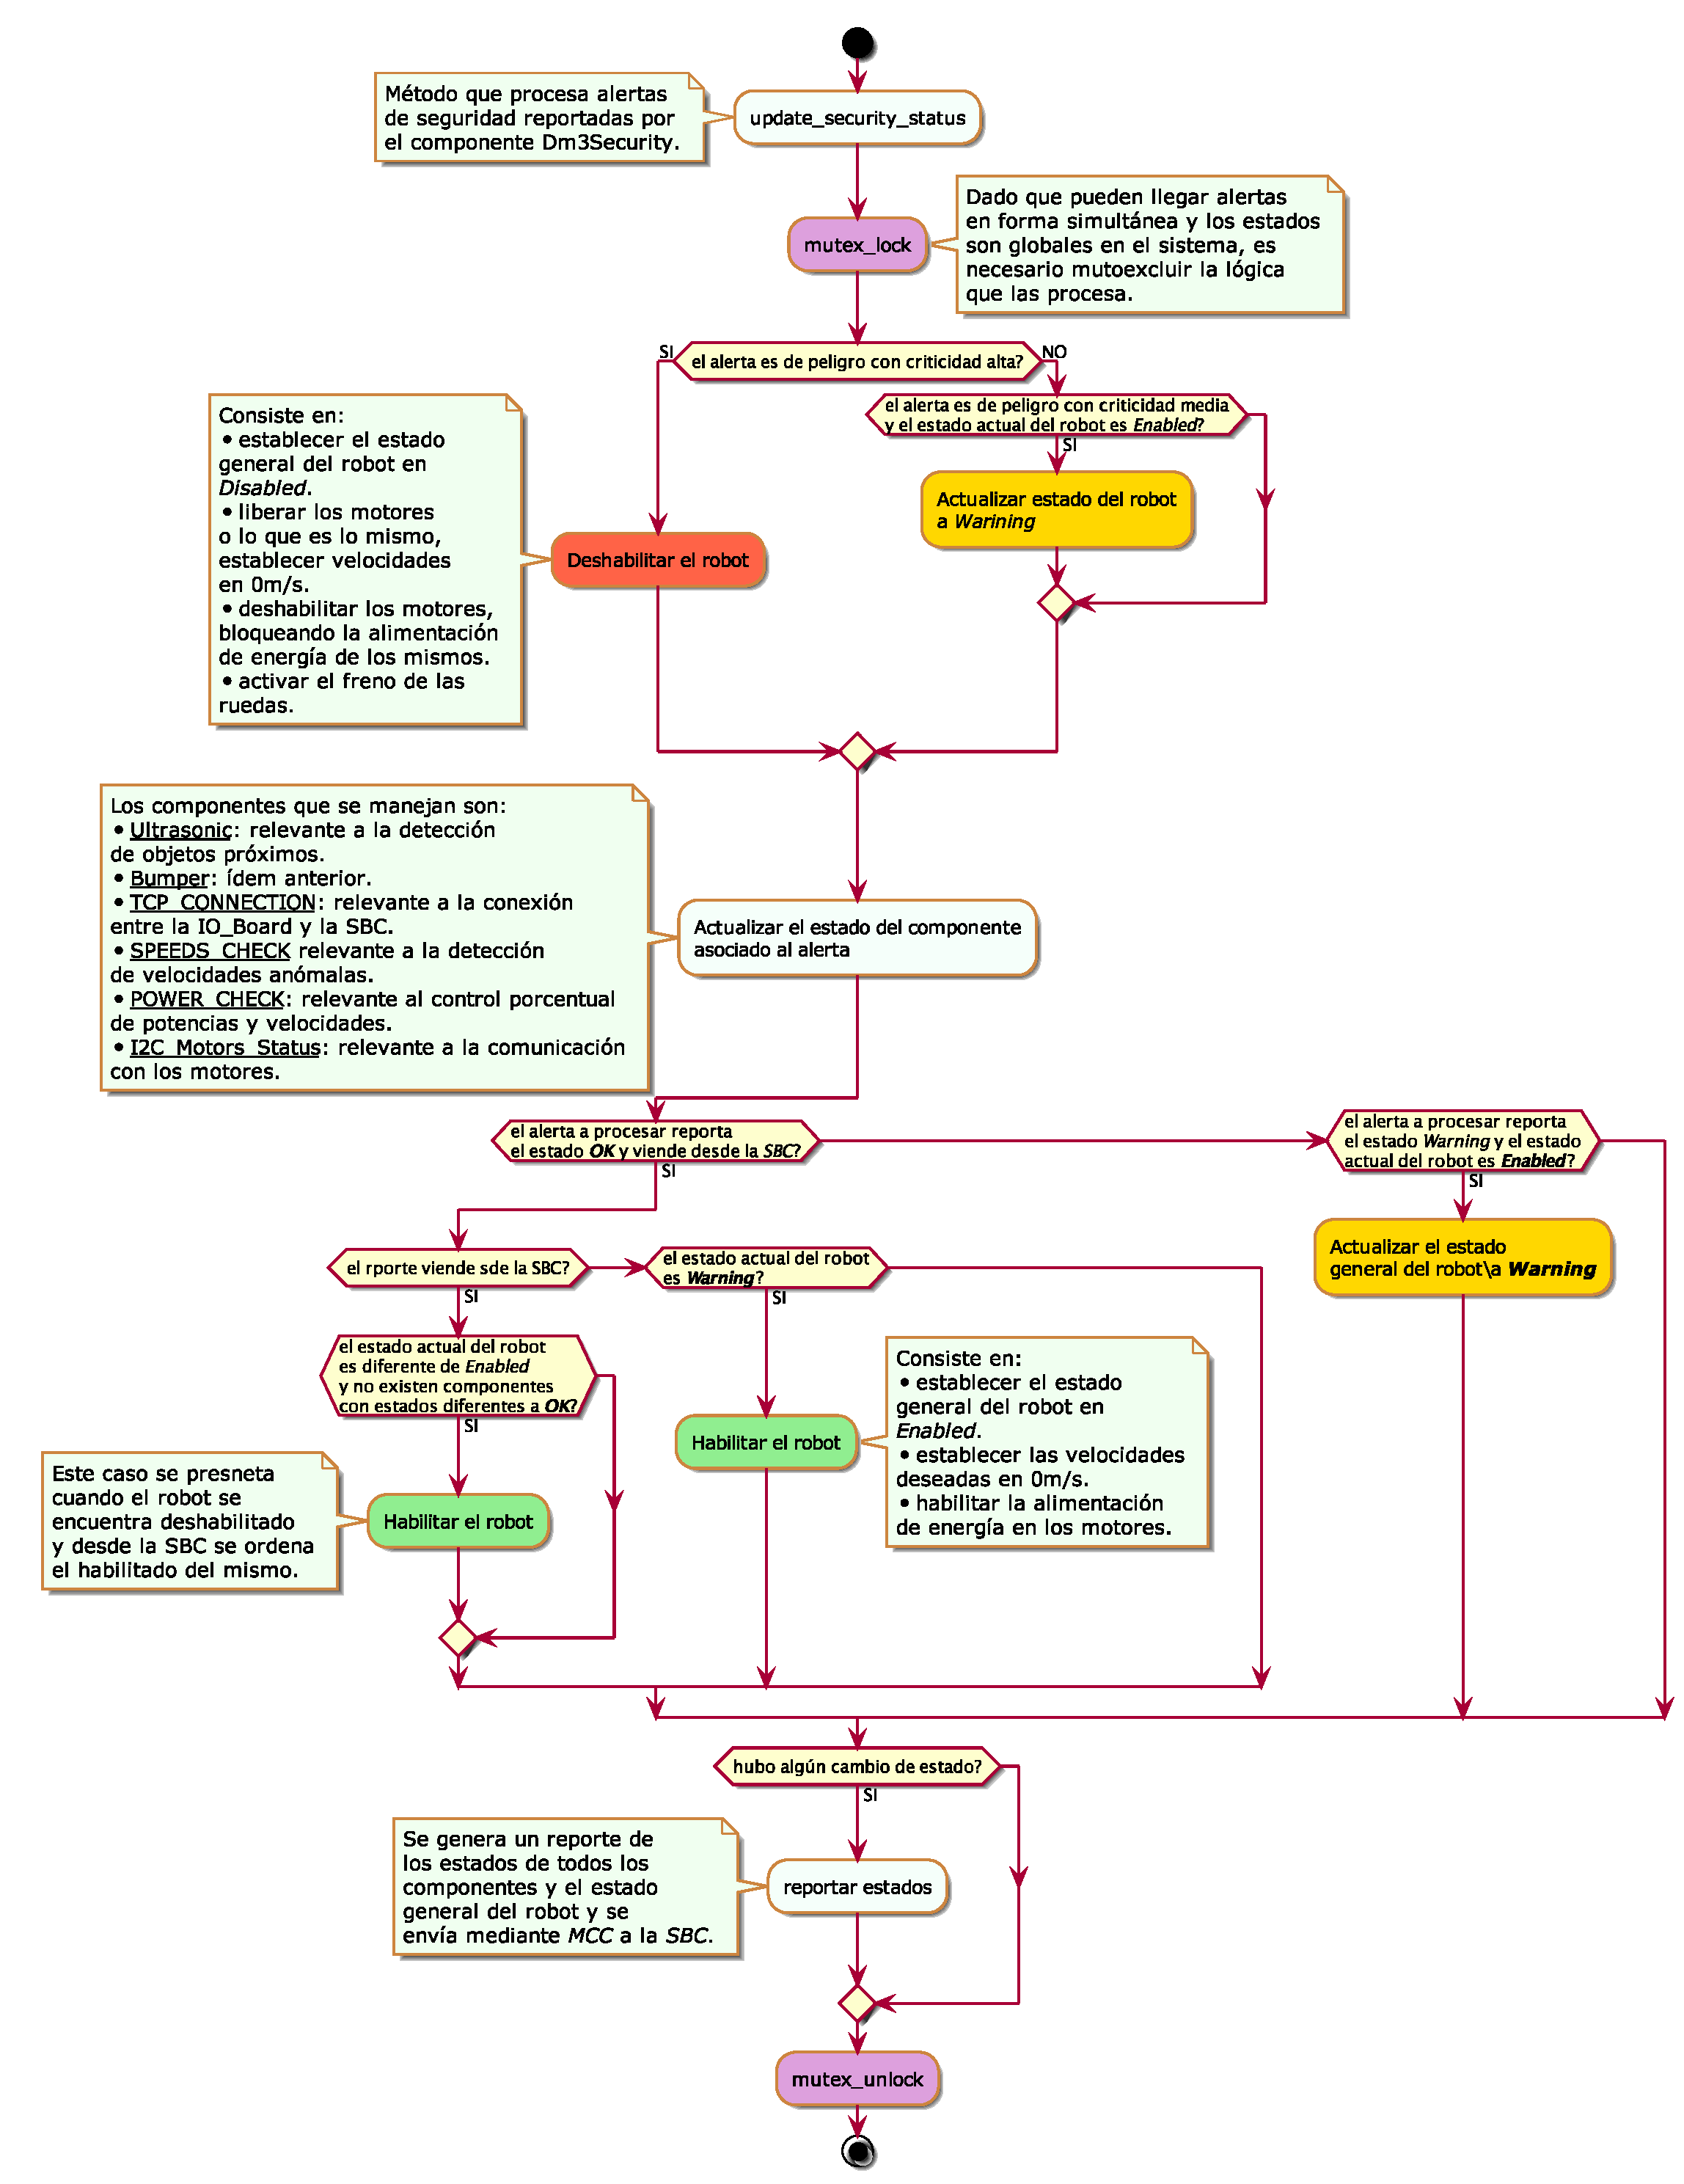
\includegraphics[width=0.8\textwidth]{images/Diagrama_de_flujo_Dm3Security_update_status}
\caption[Diagrama de flujo del proceso de alertas de seguridad]{Diagrama de flujo del proceso de alertas de seguridad.}
\end{figure}

Por otra parte el componente Dm3Security tiene como principal responsabilidad la detección de peligro para notificarlo con la mayor eficiencia posible, es por ello que depende de los componentes:
\begin{itemize}
\item  \textul{MotorModule}, para obtener información asociada a la comunicación con los motores, las potencias establecidas y las velocidades de las ruedas.
\item  \textul{Communication}, para monitorear el estado de la conexión entre los sistemas \hl{SBC} e \hl{IOBoard}.
\item  \textul{Ultrasonic}, para detectar objetos próximos. Este componente genera una interrupción al sistema y notifica la distancia a la que detecta un objeto.
\item  \textul{Bumper}, detecta el contacto con un objeto y al igual que el ultrasonido también genera una interrupción al sistema notificando la colisión.
\end{itemize}

\subsection{Detección de Objetos Próximos} \label{sec:Implementacion :: detección de objetos próximos}
Se implementaron dos mecanismos para la detección de objetos próximos, uno utilizando sensores de ultrasonido enfocado en la prevención del accidente, y el otro utilizando sensores de contacto enfocado en detectar la colisión y minimizar el peligro del accidente.

\subsubsection{Detección con sensores de ultrasonido}
El componente Dm3Security implementa una rutina que atiende las interrupciones generadas por el componente Ultrasonic reportando las distancias de los objetos detectados. Este componente Ultrasonic es simplemente un manejador del dispositivo \hl{Referencia al Ultrasonido} que emite un sonido y en función del tiempo que transcurre hasta recibir el eco de la onda emitida, debido al choque de ésta con un objeto, es capaz de determinar a qué distancia se encuentra el objeto que hizo rebotar a la onda.

El mecanismo desarrollado realiza un filtro a las señales reportadas por el sensor, de forma de suprimir variaciones muy rápidas en estas, seguramente a consecuencia de errores en el sensado. El filtro en cuestión es denominado \hl{Filtro paso bajo} de primer orden que consiste en:

\begin{center}
$dist = dist_{anterior} + \alpha * (dist_{actual} - dist_{anterior})$ 
\end{center}
siendo $\alpha$ un valor pequeño configurado en el encabezado del componente Dm3Security con el nombre \textit{ULTRASONIC\_FILTER\_ALPHA}.

Una vez que la señal fue filtrada se procede a evaluar si se ha detectado un objeto dentro del rango de alerta, es decir si la distancia reportada es inferior o igual a la distancia mínima permitida, configurada también en el encabezado del componente Dm3Security con el nombre \textit{ULTRASONIC\_MIN\_FRONT\_DIST}. A continuación se presenta un diagrama de flujo describiendo el mecanismo.

\begin{figure}[H]
\centering
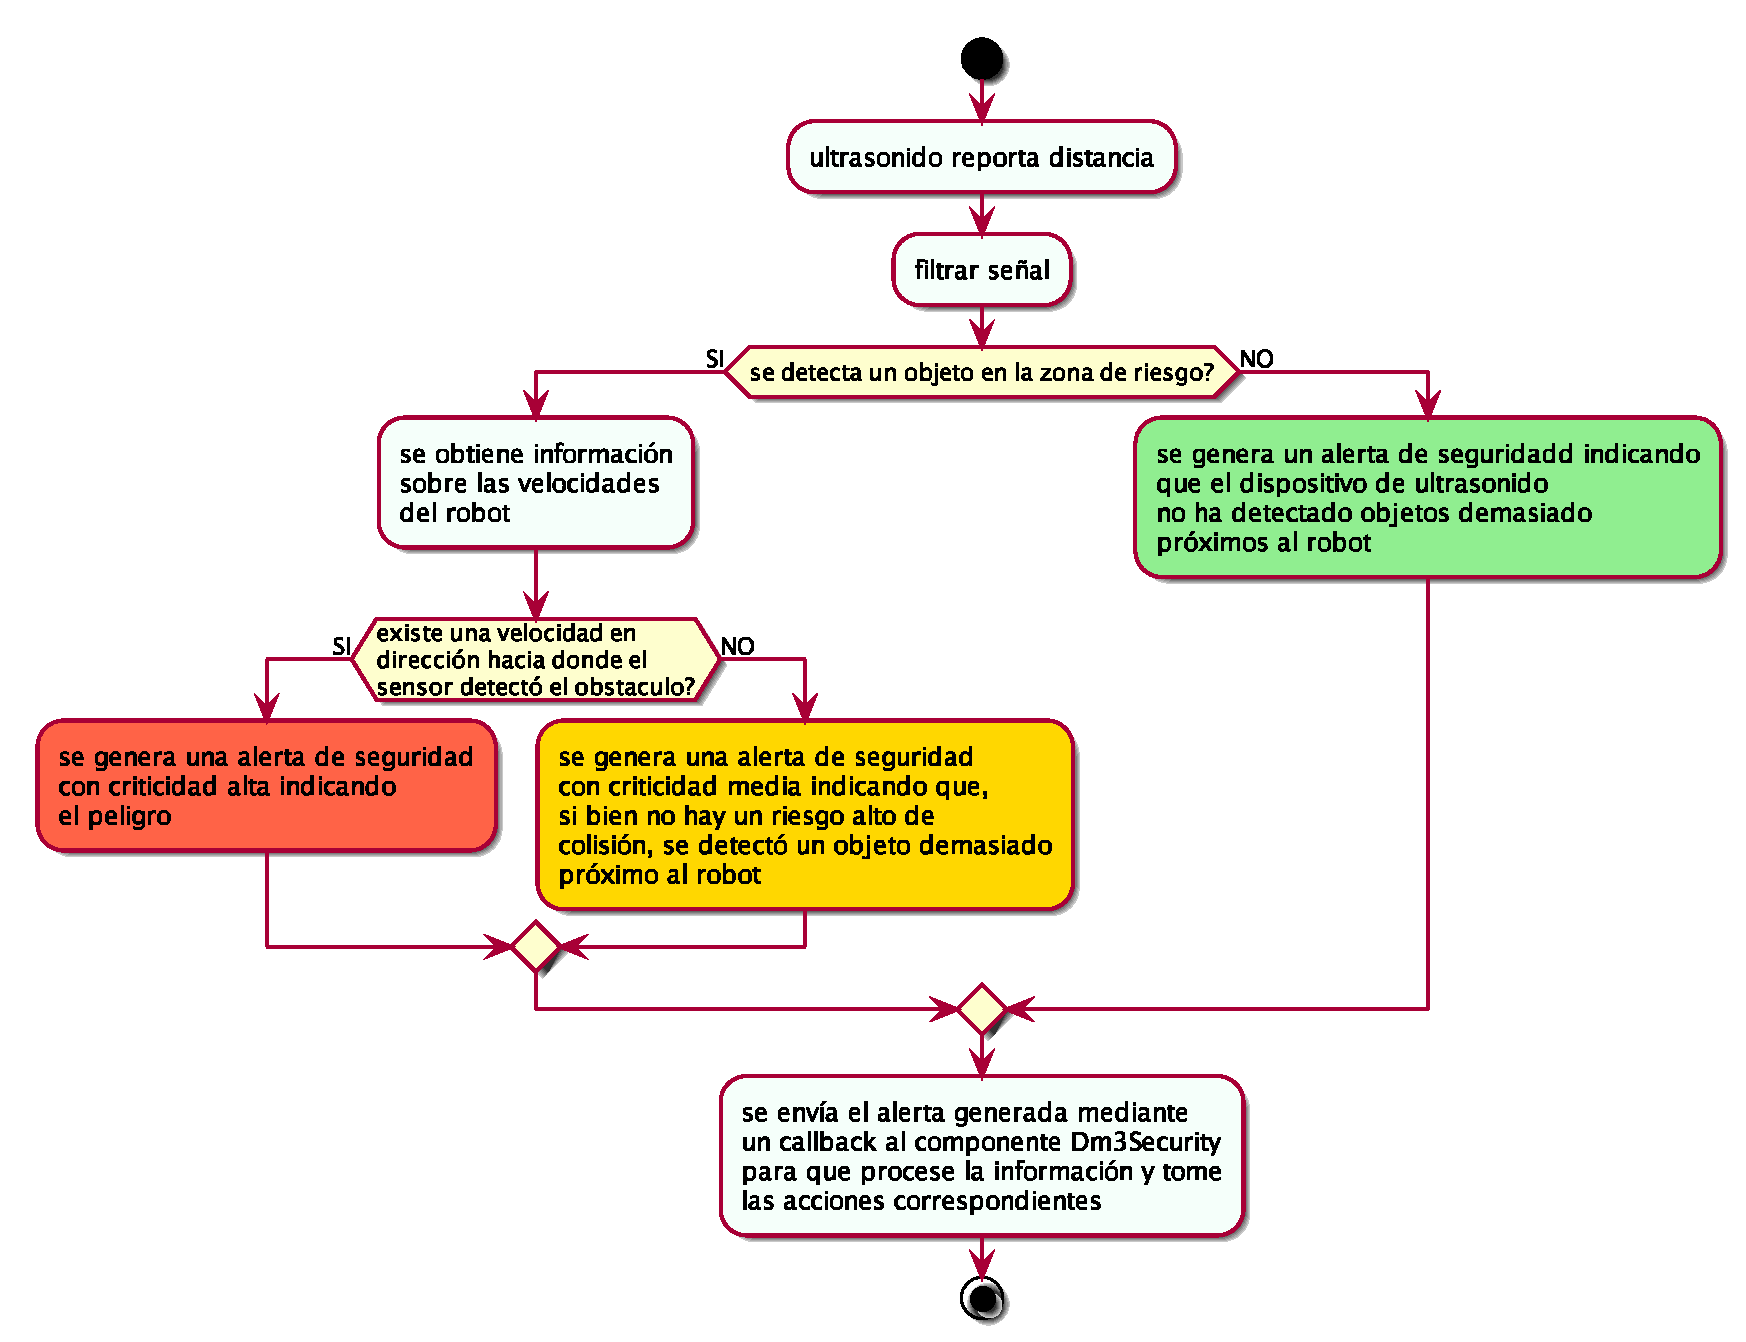
\includegraphics[width=0.8\textwidth]{images/Diagrama_de_flujo_Dm3Security_Ultrasonic}
\caption[Diagrama de flujo - Detección de objetos próximos con Ultrasonido]{Diagrama de flujo - Detección de objetos próximos con Ultrasonido.}
\end{figure}

\subsubsection{Detección con sensores de contacto} \label{sec:Implementacion :: detección de objetos próximos :: Contacto}
Este tipo de sensores, como ya se ha mencionado, actúa al momento de la colisión y es muy importante que el sistema de control esté al tanto de lo ocurrido y tome acciones lo antes posible. Es por ello que el mecanismo es bien eficiente en cuanto a la detección y reporte de lo detectado.

\begin{figure}[H]
\centering
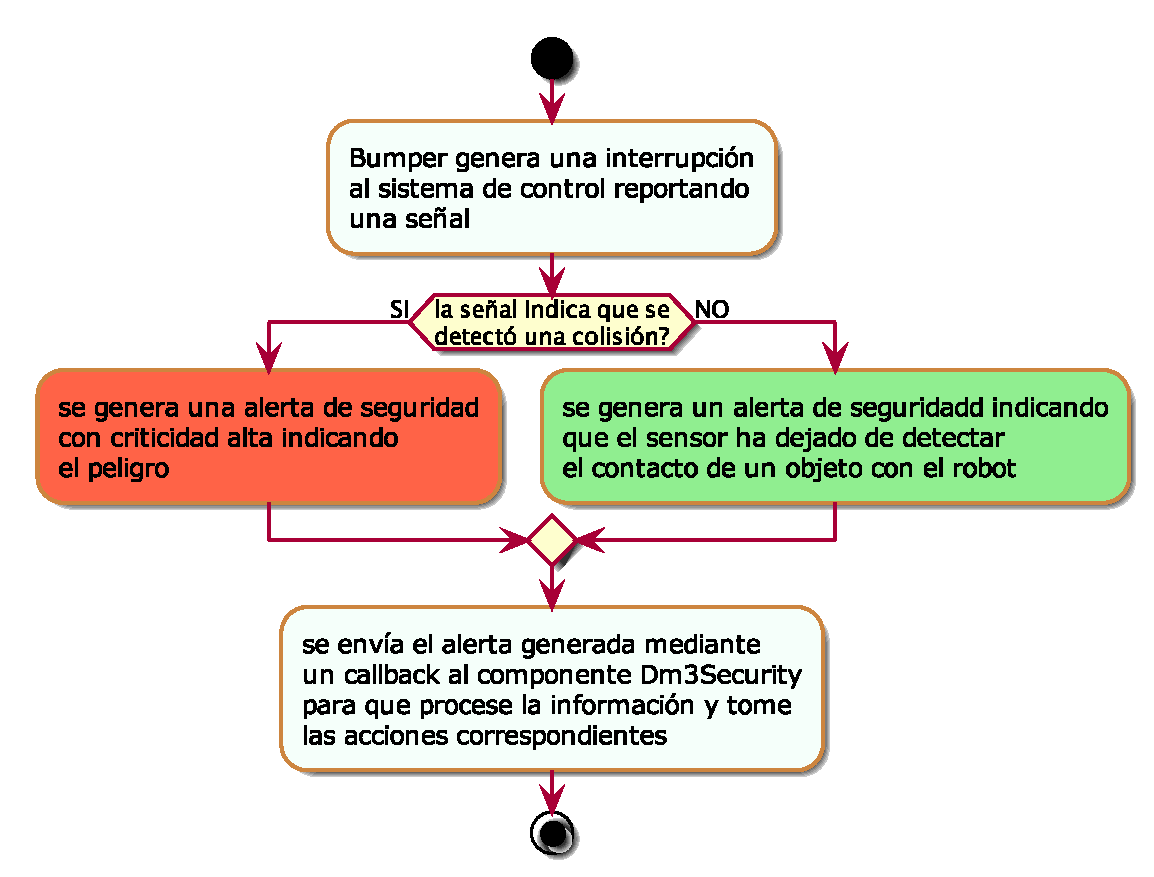
\includegraphics[width=0.8\textwidth]{images/Diagrama_de_flujo_Dm3Security_Bumper}
\caption[Diagrama de flujo - Detección de objetos con sensores de contacto]{Diagrama de flujo - Detección de objetos sensores de contacto.}
\label{fig:Diagrama de flujo - Detección de objetos con sensores de contacto}
\end{figure}

Como se observa en la Figura \ref{fig:Diagrama de flujo - Detección de objetos con sensores de contacto} este mecanismo detecta tanto cuando se presiona el sensor de contacto como cuando se deja de presionar, valiéndose de interrupciones. Cabe destacar que para evitar rebotes al presionar y liberar el sensor, y el consiguiente disparo de sucesivas interrupciones, se maneja una variable de tiempo (configurada con un valor muy pequeño) durante la cual el mecanismo no atiende eventos del sensor. Luego de transcurrido este tiempo el mecanismo se vuelve a habilitar.

\subsection{Detección de Velocidades y Potencias Anómalas}
En lo que respecta al control de velocidades se desarrolla un mecanismo de control para garantizar que el robot no se desplazará a velocidades mayores a la máxima permitida.
También se desarrolla un mecanismo para controlar que la potencia entregada a los motores es coherente con la velocidad reportada por los sensores de las ruedas. Este mecanismo es de utilidad para detectar atascamientos del robot o simplemente sobrecarga de los motores.

\subsubsection{Control de velocidad máxima} \label{sec: Control de velocidad máxima}
A continuación se presenta un diagrama que ilustra el flujo de acciones desarrolladas en el mecanismo de control de velocidades máximas.

\begin{figure}[H]
\centering
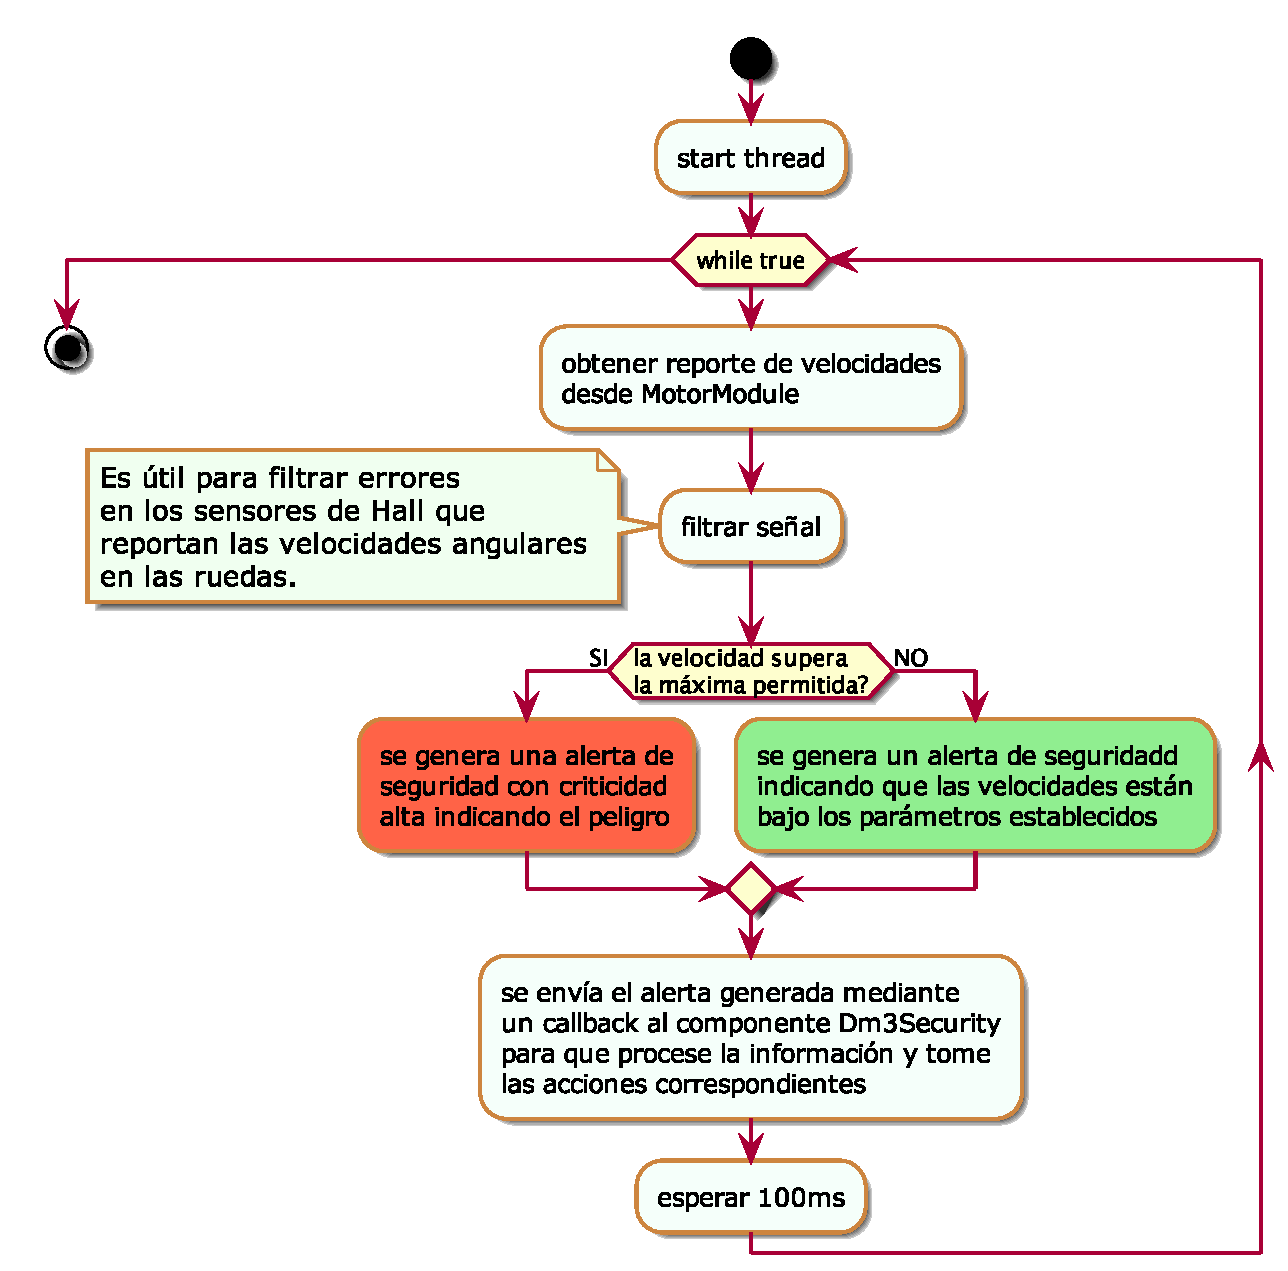
\includegraphics[width=0.8\textwidth]{images/Diagrama_de_flujo_Dm3Security_Speeds}
\caption[Diagrama de flujo - Control de velocidad máxima]{Diagrama de flujo - Control de velocidad máxima.}
\label{fig: Diagrama de flujo - Control de velocidad máxima}
\end{figure}

Para filtrar errores de medición que realizan los \hl{sensores de Hall} sobre las ruedas del robot, se desarrolló el filtro que se menciona en el diagrama de la figura \ref{fig: Diagrama de flujo - Control de velocidad máxima}. El mismo consiste en considerar el conjunto de las últimas \textit{SPEEDS\_CHECK\_WINDOW\_SIZE} velocidades reportadas, siendo este parámetro un valor configurado en el encabezado del componente Dm3Security, y calcular la velocidad promedio entre ellas. Luego esta velocidad será comparada contra la máxima velocidad permitida, valor que también se configura en el encabezado del componente Dm3Security con el nombre \textit{SPEED\_MAX\_VALUE\_ALLOWED}.

\subsubsection{Control de potencias}
El mecanismo de controles de potencia consiste en contrastar, en valores porcentuales, a la potencia establecida en los motores con la velocidad alcanzada por el robot. A continuación se presenta un diagrama que ilustra el flujo desarrollado.

\begin{figure}[H]
\centering
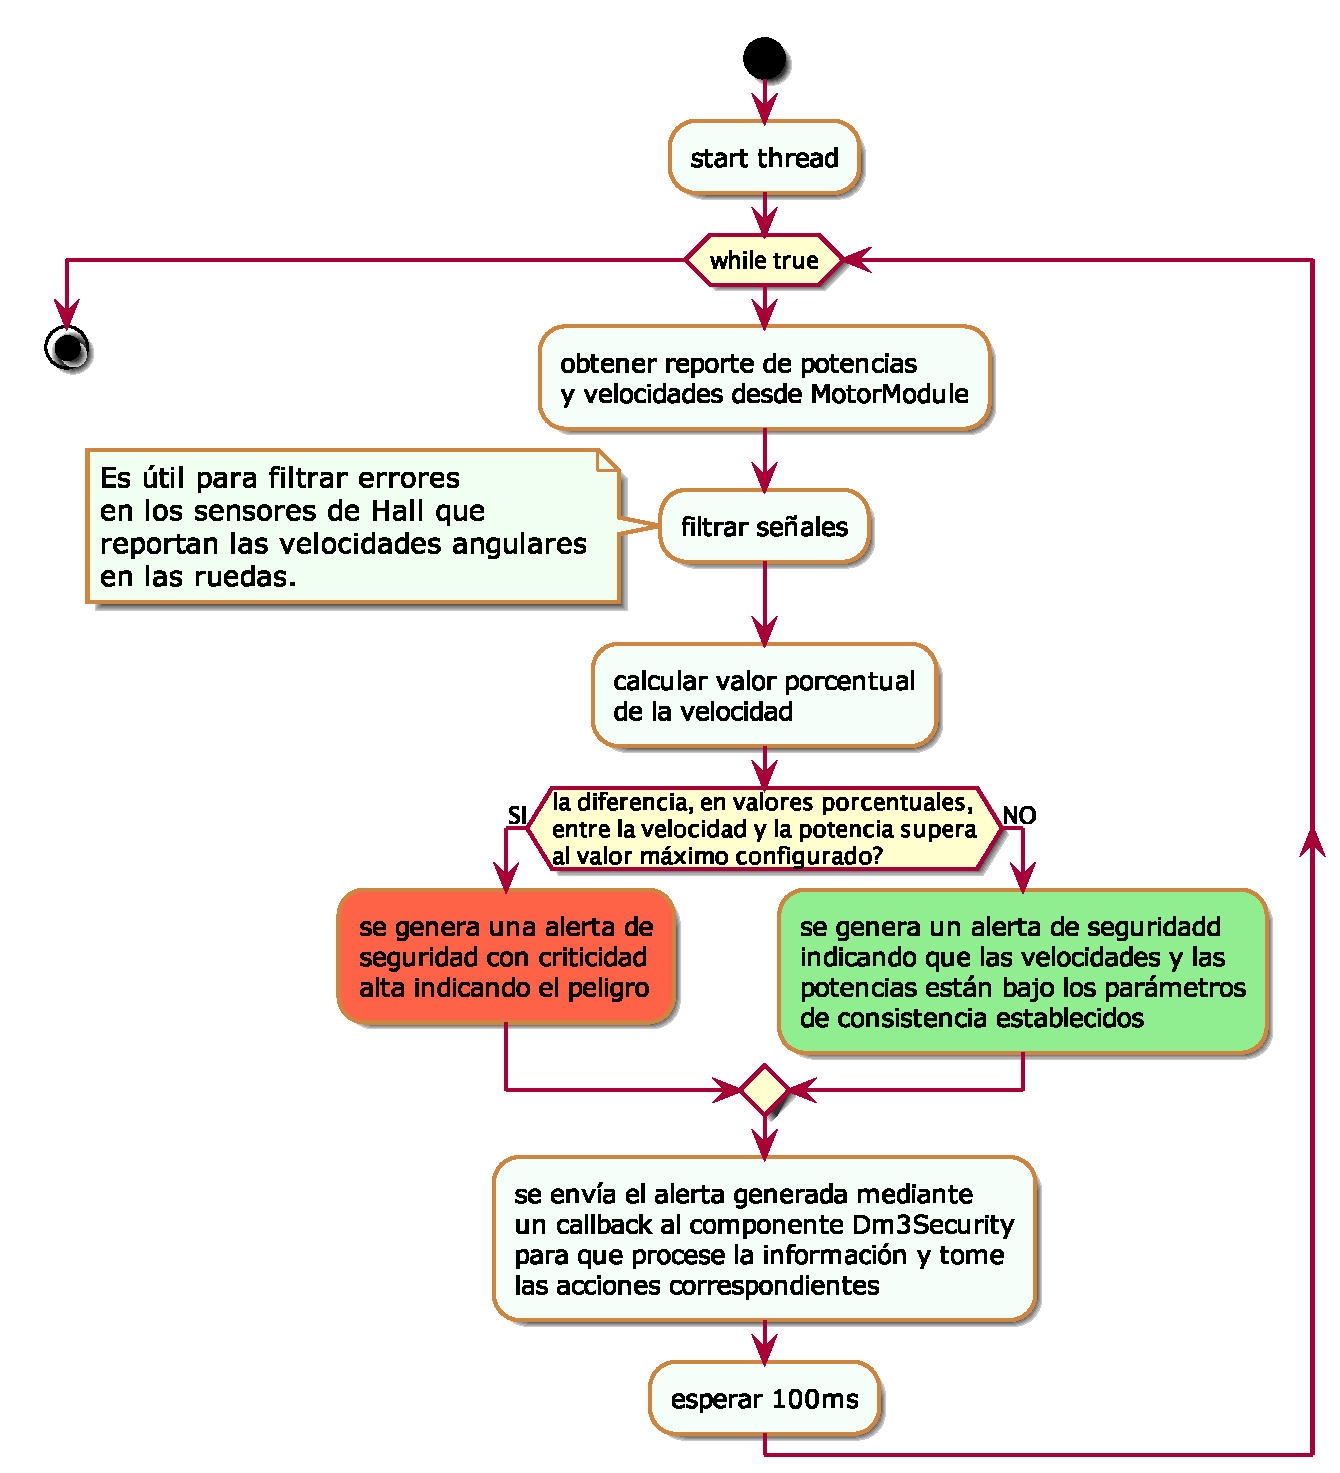
\includegraphics[width=0.8\textwidth]{images/Diagrama_de_flujo_Dm3Security_Pows}
\caption[Diagrama de flujo - Control de potencias]{Diagrama de flujo - Control de potencias.}
\label{fig: Diagrama de flujo - Control de potencias}
\end{figure}

El desarrollo de este algoritmo es ejecutado por el mismo hilo y en el mismo bucle que implementa al control de velocidades máximas. Esto permite implementar dos algoritmos que requieren del análisis de información en común siendo más eficientes con el consumo de recursos (por ejemplo con los ciclos de procesamiento y con la memoria para almacenar la información a ser analizada).

Para filtrar errores en las mediciones de las velocidades se utiliza el proceso de filtrado que se describe en la sección anterior (\ref{sec: Control de velocidad máxima}).

El cálculo que determina si la velocidad y potencia reportadas son consistentes en un funcionamiento seguro del robot consiste en:
\begin{itemize}
\item convertir el valor de la velocidad reportada \SI{}{\metre/\second} en un valor porcentual para poder contrastarlo con el valor porcentual de potencias establecidas en los motores. Vale la pena aclarar que los valores reportados de potencia son expresados ya en medidas porcentuales. Para realizar esta conversión se implementa:
\begin{itemize}
\item[•] $vel_{percent} =  \frac{ vel_{mps}  \cdot  100}{SPEED\_MAX\_VALUE}$, siendo \textit{SPEED\_MAX\_VALUE} un parámetro configurado en el encabezado del componente Dm3Security en base a la velocidad máxima soportada por el hardware del robot.
\end{itemize}
\item comparar la diferencia entre los valores porcentuales de velocidad y potencia contra el parámetro \textit{MAX\_POWS\_SPEED\_DESVIATION} configurado en el encabezado del componente Dm3Security. Este parámetro indica la diferencia máxima que puede existir entre los valores porcentuales de velocidad y potencia, en caso de que la diferencia sea mayor se disparará un alerta de seguridad indicando el peligro detectado.
\end{itemize} 

\subsection{Monitoreo y Recuperación de la Conexión}

En lo que respecta al tópico monitoreo de la conexión se implementan dos procesos, uno que realiza un monitoreo de la conexión TCP con la SBC y otro que realiza un monitoreo de errores en la conexión \hl{I2C} con los motores. Ambos procesos consisten en monitorear una conexión en particular y en caso de detectar un error generar un alerta de seguridad indicando el peligro correspondiente, en ninguno de los dos casos se implementa una corrección del error encontrado, simplemente se notifica y el componente Dm3Module tomará las medidas adecuadas.

Es importante mencionar que el Communication (ver diagrama de la figura \ref{fig: Diagrama de componentes - Firmware IO Board}) implementa un controlador para TCP que provee operaciones para enviar y recibir datos, así como también para establecer la conexión con la SBC cuando ésta se encuentre caída y el sistema de control necesite recibir o enviar datos. En caso de no poder establecerse efectivamente dicha conexión, el proceso mencionado anteriormente lo detectará y reportará un alerta de seguridad de riesgo alto que, al ser procesada por el Dm3Module, desactivará al robot. 

\subsection{Watchdog}
Componente desarrollado para operar con el módulo Watchdog provisto por en el hardware de la IOBoard. Provee las siguientes una operaciones:
\begin{itemize}
\item \textul{Constructor}: construye al componente y realiza la configuración requerida para operar con el hardware. Dentro de las configuraciones realizadas se habilita el módulo de hardware así como también se establece el tiempo máximo en el que se debe restablecer el temporizador de vigilancia. Este valor es configurado en el encabezado del componente Watchdog con el nombre \textit{toVal} y su valor por defecto está en \SI{5}{\second}.  	
\item \textul{kick}: restablece el temporizador de vigilancia con el valor configurado en el parámetro \textit{toVal}.
\item \textul{getTimeOutValue}: retorna el valor del parámetro \textit{toVal}.
\item \textul{getLastResetStatus}: retorna el motivo del último reinicio del sistema.
\end{itemize}

Este componente es utilizado por el proceso principal del sistema, donde se construye y se restablece el valor del temporizador de vigilancia. También es utilizado por el componente Dm3Security para reportar a la SBC los motivos de reinicio del sistema.

\section{Indicadores de Estado} \label{sec: Implementación :: Indicadores de Estado}
Se desarrollaron tres mecanismos para indicar estados del robot a los operarios, como se describe en la sección \ref{sec: sol prop - Indicadores de Estado}, estos indicadores son: Pantalla LCD indicando estados reportados por los mecanismos de seguridad, Sirena audible indicando un riesgo alto de seguridad y la Luz de Emergencia que indica que el robot se encuentra con la alimentación de energía activa.

\subsection{Pantalla LCD}
Desde la \hl{IO Board} se reporta el estado de todos los mecanismos de seguridad así como también el estado general del robot. El mensaje es procesado en la \hl{SBC} y finalmente enviado a la Pantalla LCD don es presentado a los operarios. El siguiente diagrama de actividad describe dicho flujo de procesamiento.

\begin{figure}[H]
\centering
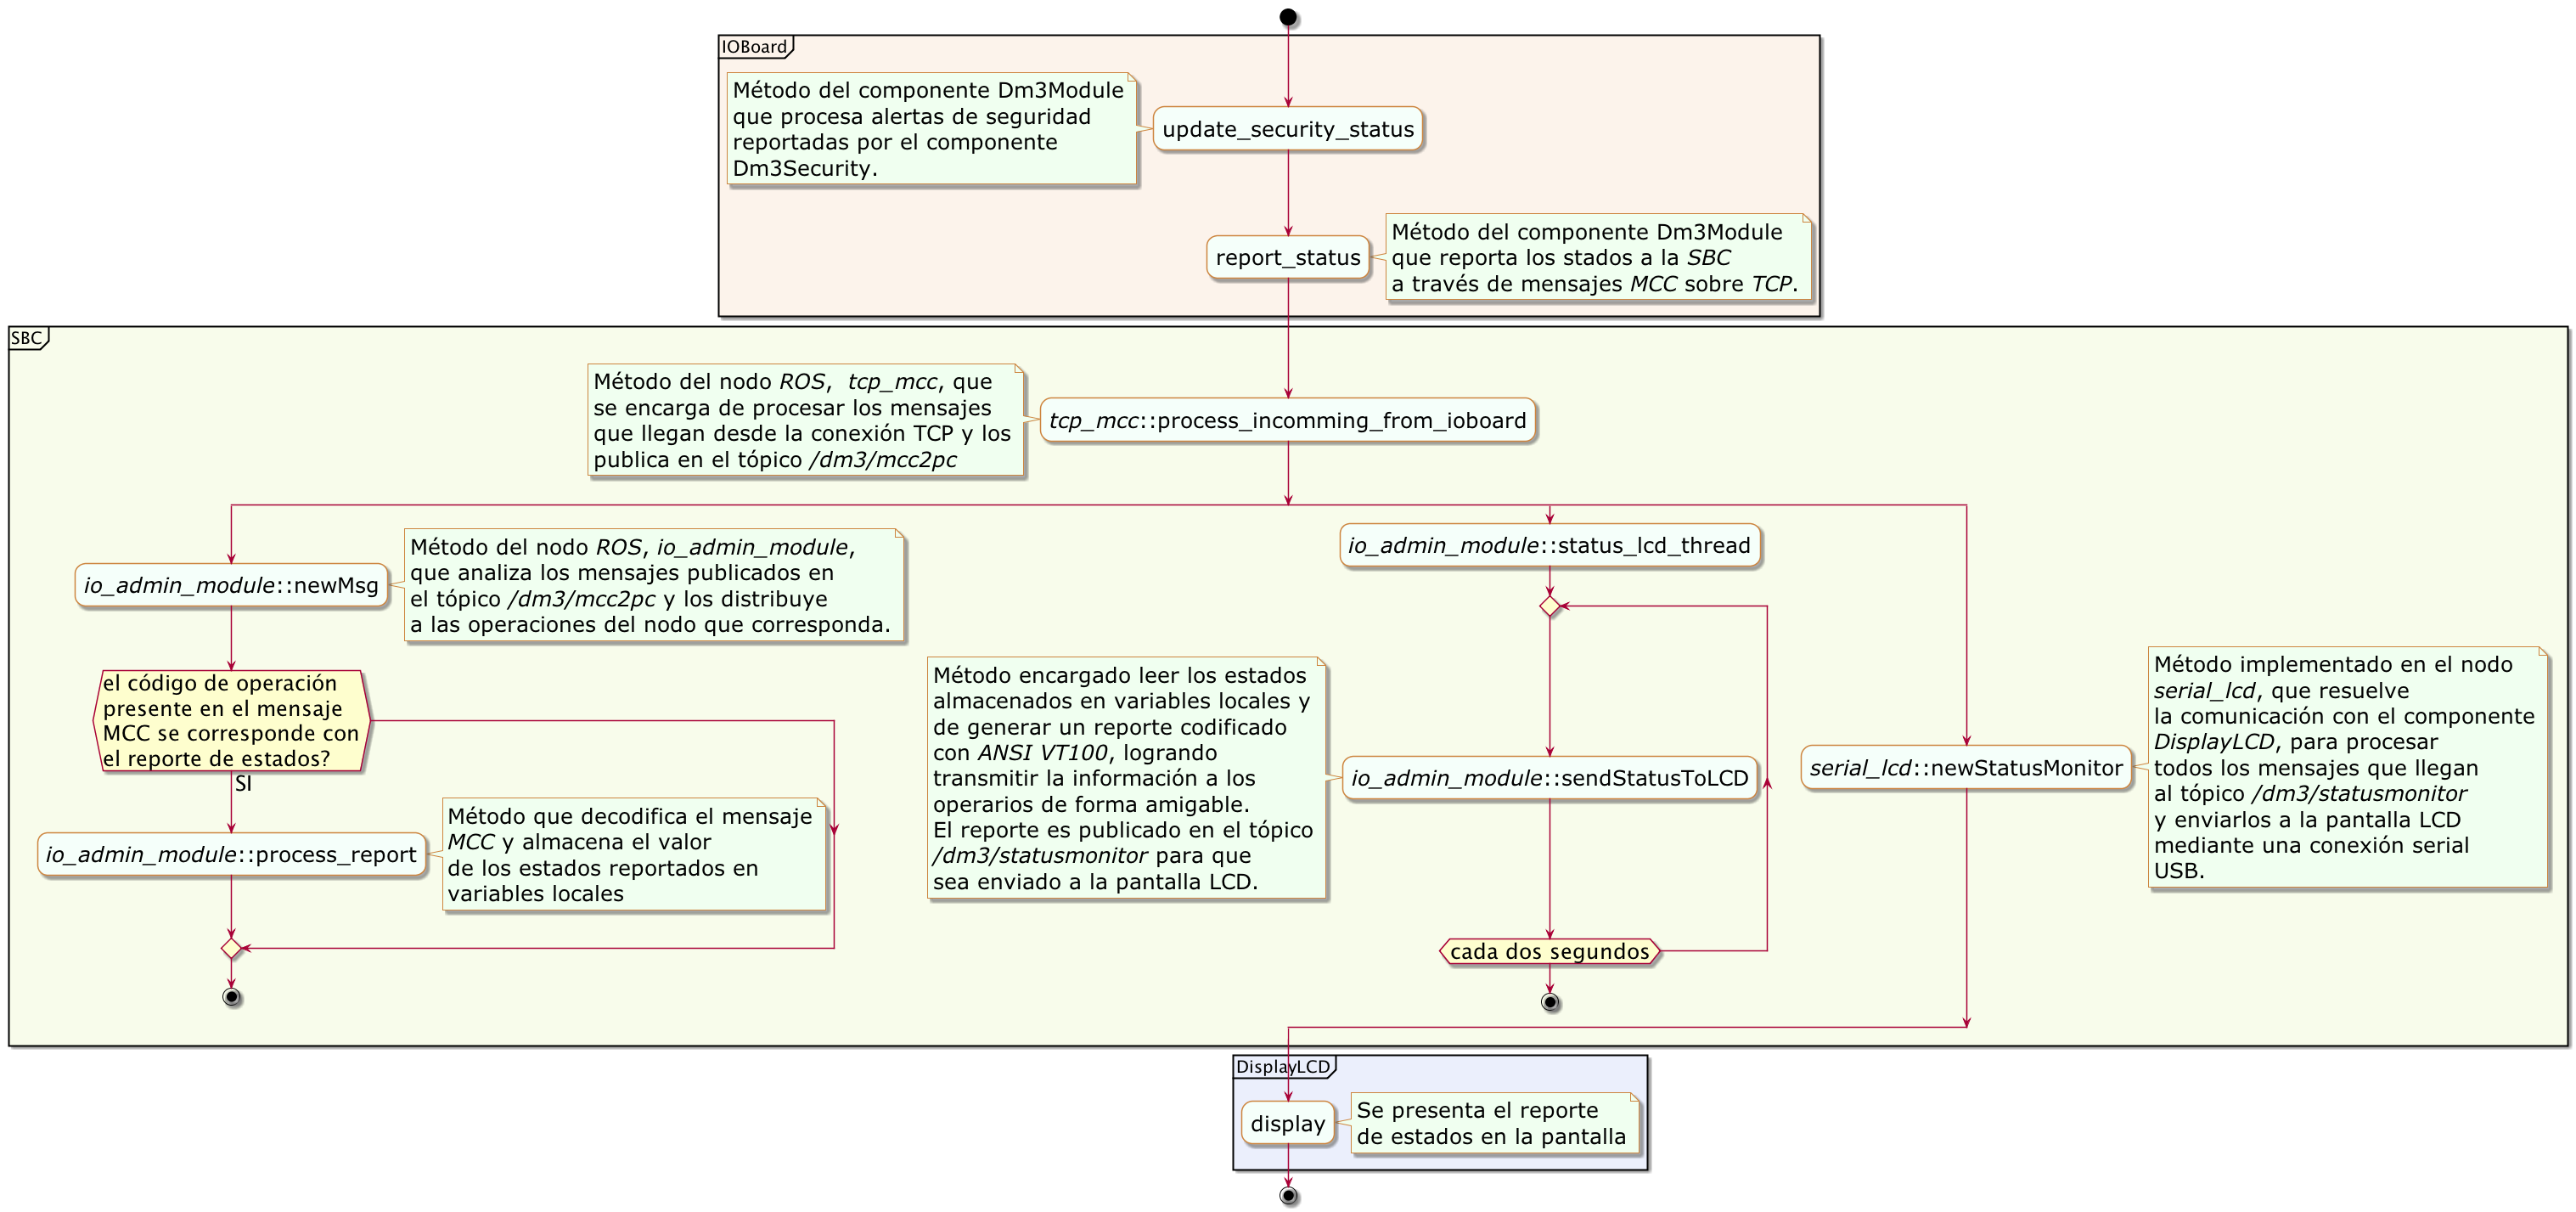
\includegraphics[width=\textwidth]{images/Diagrama_de_flujo_indicadores_de_estados}
\caption[Diagrama de flujo - Indicadores de estados, pantalla LCD]{Diagrama de flujo - Reporte de estados en la pantalla LCD.}
\label{fig: Diagrama de flujo - Indicadores de estados Pantalla LCD}
\end{figure}

\subsection{Sirena audible}
Este dispositivo alerta de un potencial riesgo o eventualmente del peligro ocasionado por una falla en el sistema.
La sirena es activada cuando tenemos un alerta de seguridad de criticidad media, que es en el momento en el que el robot pasa a estado \textit{Warning}, o cuando tenemos un alerta de seguridad de criticidad alta dónde el robot se encontrará deshabilitado (estado \textit{Disabled}). En cualquier otro caso la sirena estará desactivada.
 
\chapter{Evaluación Experimental}
En esta sección se presentan las pruebas realizadas para evaluar el desarrollo de los mecanismos de seguridad sobre un prototipo experimental. En la Sección 6.1 se describen la pruebas funcionales realizadas y en la Sección 6.2 las pruebas de rendimiento, finalmente, en la Sección 6.3 se presenta la evaluación de los resultados obtenidos.

\section{Pruebas Funcionales}
\subsection{Control de Distancia}
A continuación se describen pruebas realizadas para validar el mecanismo de control de distancias.

Como se describió en \ref{sec:Sol Prop :: detección de velocidades y potencias anómalas} y \ref{sec:Implementacion :: detección de objetos próximos} el mecanismo se apoya en el uso de sensores de ultrasonido para medir distancias a obstáculos presentes en la vecindad del robot. Para la prueba se colocó un sensor ultrasonido en la plataforma prototipo enfocando hacia adelante, a una distancia de \SI{40}{\centi\metre} desde el frente del robot y a una altura de \SI{45}{\centi\metre} desde el piso (\SI{35}{\centi\metre} desde el chasis del robot) como se observa en las figuras~\ref{fig:vistaFrontal} y~\ref{fig:vistaSuperior}.

\begin{figure}[H]
  \centering
  \begin{minipage}[b]{0.4\textwidth}
    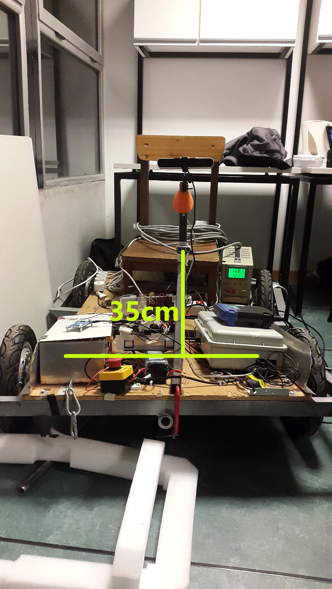
\includegraphics[width=\textwidth]{images/Chasis0_FRONT}
    \caption[Chasis 0 - Vista Frontal]{Chasis 0, vista frontal.}
    \label{fig:vistaFrontal}
  \end{minipage}
  \hfill
  \begin{minipage}[b]{0.4\textwidth}
    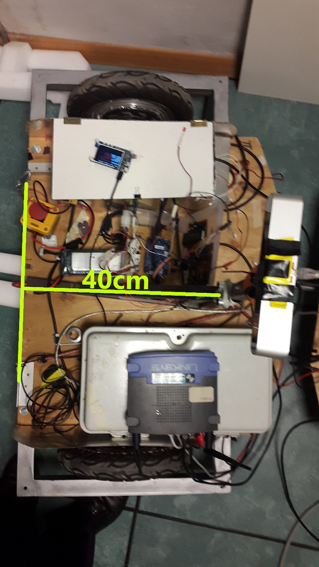
\includegraphics[width=\textwidth]{images/Chasis0_TOP}
    \caption[Chasis 0 - Vista Superior]{Chasis 0, vista superior.}
    \label{fig:vistaSuperior}
  \end{minipage}
\end{figure}

En líneas generales la prueba realizada consistió en colocar el robot a \SI{5}{\metre} de un obstáculo y en una trayectoria de colisión, para luego encenderlo y ordenarlo avanzar a distintas velocidades. Luego de disparado el mecanismo de seguridad se midió a que distancia del obstáculo quedó la parte más próxima del robot. Para todas las ejecuciones la distancia máxima tolerable configurada fue de \SI{2}{\metre}, lo que considerando la localización del sensor implica una distancia de \SI{1.6}{\metre} desde el frente del robot.

Los cuadros~\ref{table:ultrasonic025},~\ref{table:ultrasonic050},~\ref{table:ultrasonic075},~\ref{table:ultrasonic100} y~\ref{table:ultrasonic150} muestran los resultados de los experimentos para velocidades de \SI{0.25}{\metre/\second}, \SI{0.50}{\metre/\second}, \SI{0.75}{\metre/\second}, \SI{1.00}{\metre/\second} y \SI{1.50}{\metre/\second} respectivamente. Se registraron 5 ejecuciones de cada prueba.

\begin{table}
  \begin{minipage}[b]{0.4\textwidth}
    \caption[Test Distancia Ultrasonidos - Velocidad = \SI{0.25}{\metre/\second}]{Resultados de testeo de mecanismo de control de distancia con sensor de ultrasonidos, velocidad \SI{0.25}{\metre/\second}.}
    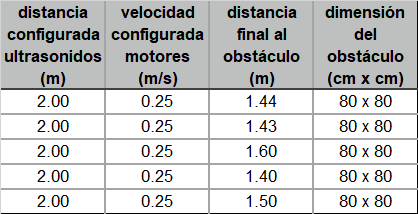
\includegraphics[width=\textwidth]{images/Test_Ultrasonic025}    
    \label{table:ultrasonic025}
  \end{minipage}
  \hfill
  \begin{minipage}[b]{0.4\textwidth}
  	\caption[Test Distancia Ultrasonidos - Velocidad = \SI{0.50}{\metre/\second}]{Resultados de testeo de mecanismo de control de distancia con sensor de ultrasonidos, velocidad \SI{0.50}{\metre/\second}.}
    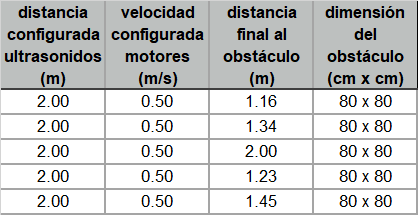
\includegraphics[width=\textwidth]{images/Test_Ultrasonic050}    
    \label{table:ultrasonic050}
  \end{minipage}
\end{table}

\begin{table}[H]
  \centering
  \begin{minipage}[b]{0.4\textwidth}
  	\caption[Test Distancia Ultrasonidos - Velocidad = \SI{0.75}{\metre/\second}]{Resultados de testeo de mecanismo de control de distancia con sensor de ultrasonidos, velocidad \SI{0.75}{\metre/\second}.}
    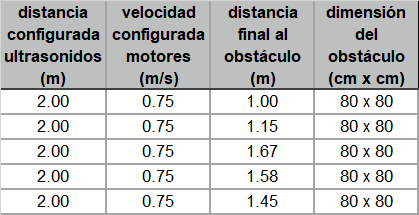
\includegraphics[width=\textwidth]{images/Test_Ultrasonic075}    
    \label{table:ultrasonic075}
  \end{minipage}
  \hfill
  \begin{minipage}[b]{0.4\textwidth}
  	\caption[Test Distancia Ultrasonidos - Velocidad = \SI{1.00}{\metre/\second}]{Resultados de testeo de mecanismo de control de distancia con sensor de ultrasonidos, velocidad \SI{1.00}{\metre/\second}.}
    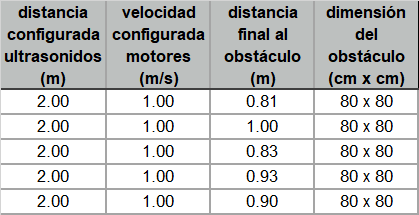
\includegraphics[width=\textwidth]{images/Test_Ultrasonic100}    
    \label{table:ultrasonic100}
  \end{minipage}
\end{table}

\begin{table}[H]
  \begin{minipage}[b]{0.4\textwidth}
  	\caption[Test Distancia Ultrasonidos - Velocidad = \SI{1.50}{\metre/\second}]{Resultados de testeo de mecanismo de control de distancia con sensor de ultrasonidos, velocidad \SI{1.50}{\metre/\second}.}  
  	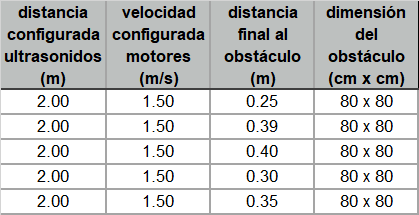
\includegraphics[width=\textwidth]{images/Test_Ultrasonic150}  	
  	\label{table:ultrasonic150}
  \end{minipage}
\end{table}

En la figura ~\ref{fig:plotUltrasonic} se presentan los resultados del conjunto de pruebas en una gráfica. Como se observa, y era de esperar, la línea de tendencia\footnote{Se asumió una tendencia lineal.} muestra que a mayor velocidad la distancia a la que se detiene el robot disminuye, no obstante esto aun para la mayor velocidad evaluada el robot se detuvo antes de colisionar con el obstáculo. Proyectando la tendencia, a velocidades superiores a los \SI{2.00}{\metre/\second} aprox. (el corte del eje Distancia al Obstáculo ocurre en v $\cong$ \SI{1.94}{\metre/\second}) el robot colisionaría con el obstáculo.

\begin{figure}[H]
  \centering
  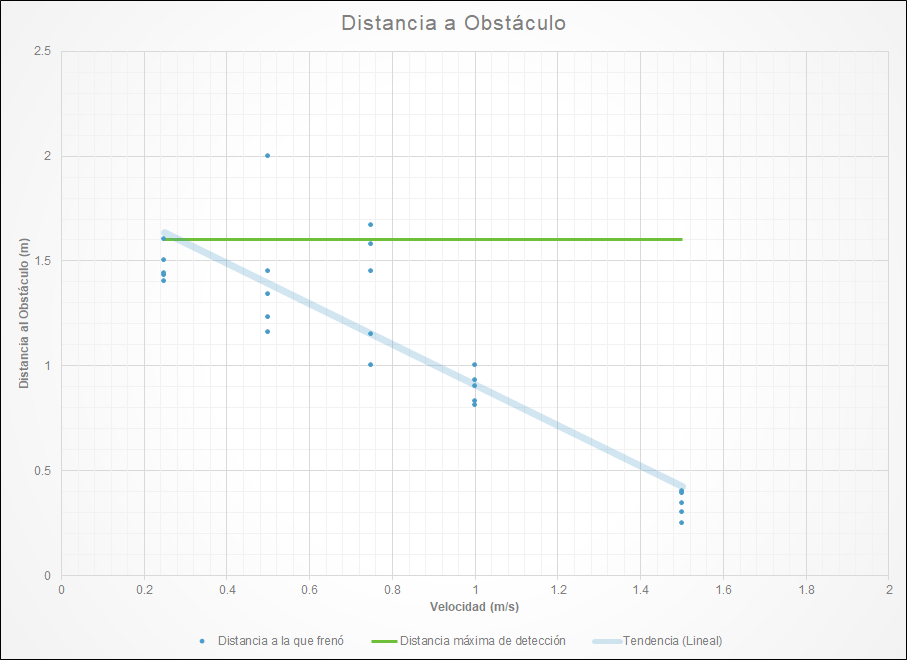
\includegraphics[width=0.5\textwidth]{images/Plot_UltrasonicBrake}
  \caption[Pruebas del control de distancia]{Pruebas del control de distancia.}
  \label{fig:plotUltrasonic}
\end{figure}

\subsection{Control de Límite de Velocidad} \label{sec:Exp Eval :: Control Limite Velocidad}
Se realizo este experimento para validar el control que verifica que la velocidad alcanzada por el robot no supera un máximo predefinido (ver Sección \ref{sec: Control de velocidad máxima}), de aquí en mas y a los efectos de este experimento llamaremos a dicha velocidad ``velocidad segura''. El experimento consistió entonces en ejecutar un script que enviase al robot cada un segundo velocidades cada vez mayores a partir de los \SI{0.50}{\metre/\second} y hasta los \SI{1.80}{\metre/\second} habiendo configurado el parámetro velocidad segura, considerando la evaluación sobre el control de distancias realizada en \ref{sec:Exp Eval :: Evaluación Resultados}, en \SI{1.50}{\metre/\second}.

\begin{figure}[H]
  \centering
  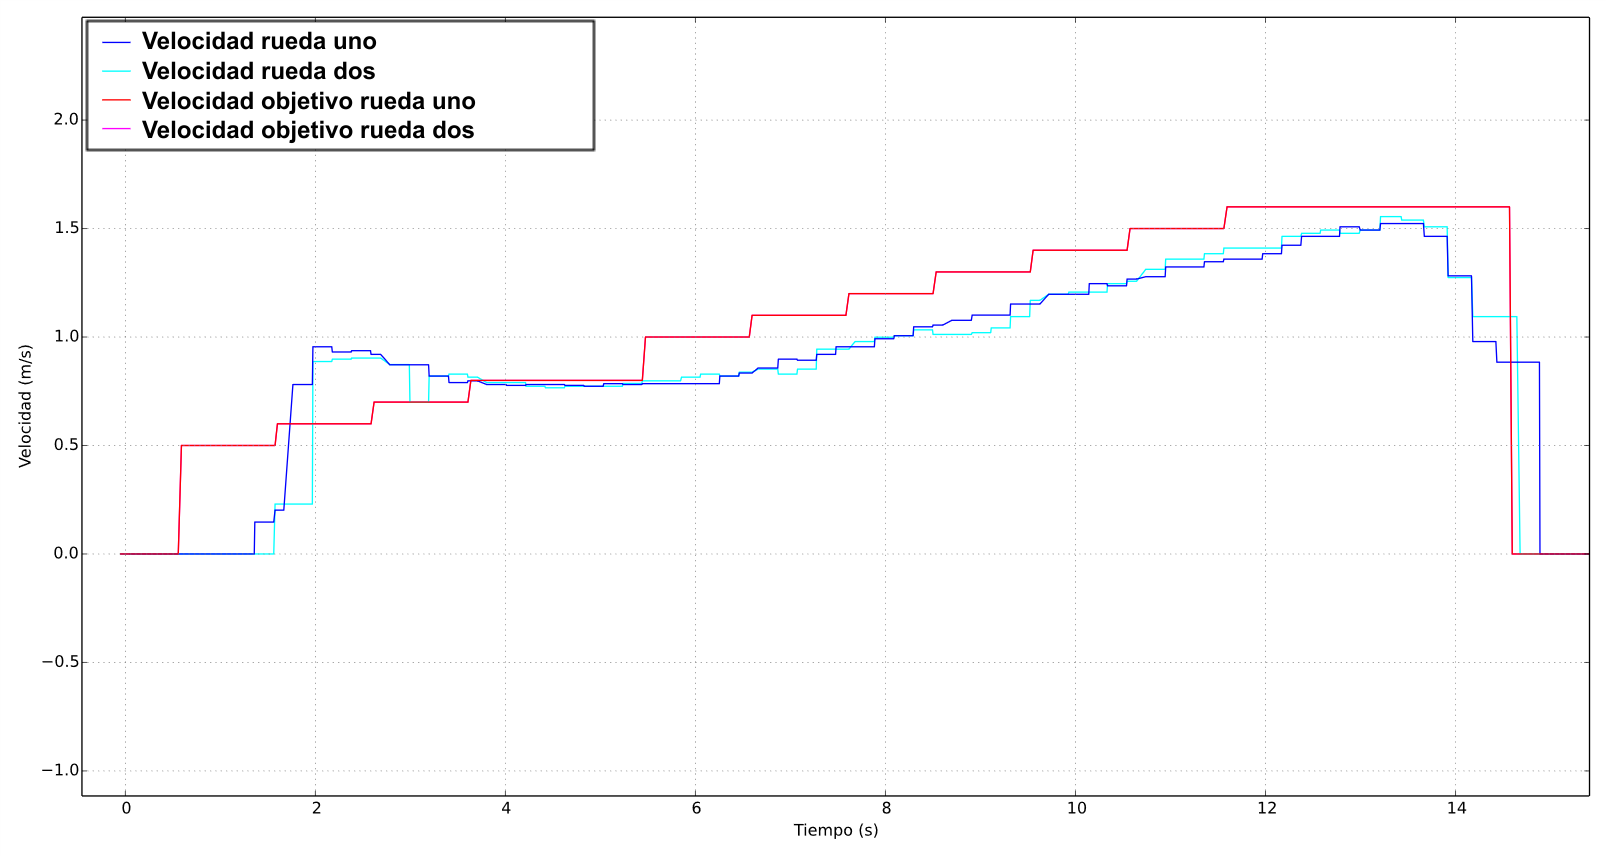
\includegraphics[width=0.5\textwidth]{images/Plot_SpeedBrake}
  \caption[Prueba del Control de Límite de Velocidad]{Prueba del Control de Límite de Velocidad.}
  \label{fig:plotSpeedTest}
\end{figure}

En la gráfica de la figura \ref{fig:plotSpeedTest} se muestra una de las ejecuciones del experimento. Se observa claramente en la misma que luego de que la velocidad supera los \SI{1.50}{\metre/\second} esta desciende dramáticamente hasta \SI{0.00}{\metre/\second}, lo que ha ocurrido aquí es que el mecanismo de seguridad se ha disparado y ha deshabilitado el robot. Este resultado fue observado consistentemente para todas las pruebas realizadas.

\subsection{Control de la Relación entre Potencia y Velocidad} \label{sec: Relación Potencia Velocidad}
Se describe la prueba llevada adelante para inferir como es la relación entre la potencia enviada a los motores y la velocidad desarrollada por el robot. Esta prueba se llevo adelante para luego, habiendo observado los resultados obtenidos, determinar un valor razonable para el parámetro utilizado en el mecanismo de seguridad que controla el ``gap'' entre estos dos atributos. Se describen también los experimentos realizados para validar el mecanismo de seguridad propuesto.

El experimento consistió en ejecutar scripts dándole ordenes al robot de que se moviese a distintas velocidades, obteniendo como salida de las ejecuciones gráficas que muestran en el eje de las abscisas el tiempo y en el eje de las ordenadas las potencias enviadas a los motores y las velocidades alcanzadas por las ruedas como un porcentaje de sus valores máximos posibles. Se utilizo para esta prueba sólo el chasis frontal del robot suspendido en el aire.

\begin{figure}[H]
\centering
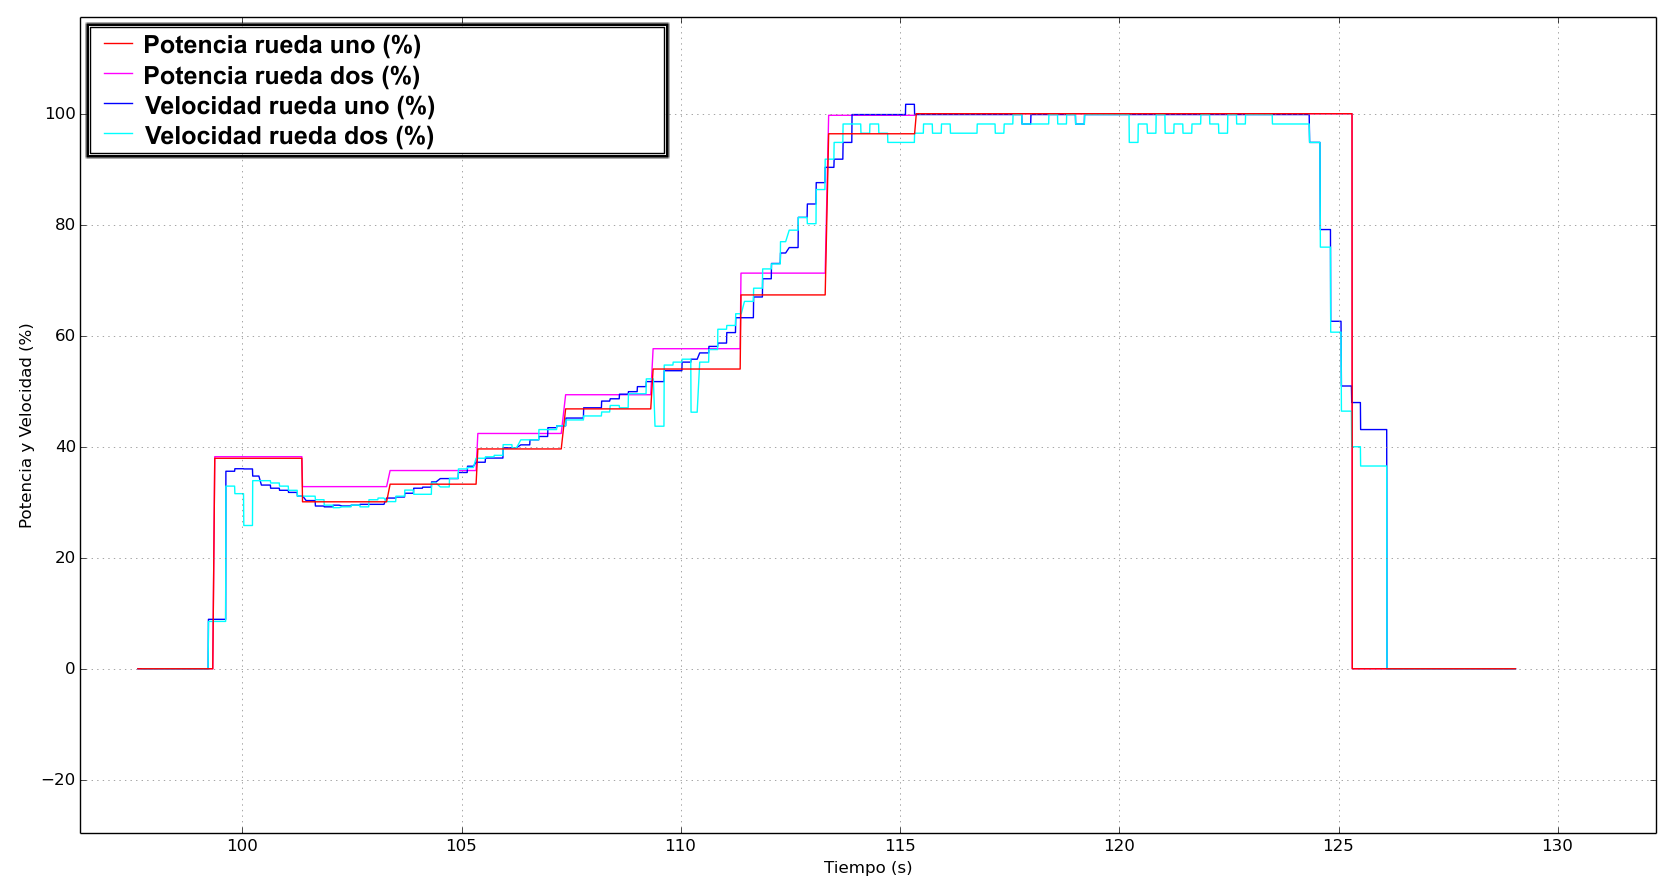
\includegraphics[width=0.5\textwidth]{images/Plot_IncreasingPowvsSpeed}
\caption[Prueba de Relación entre Potencia y Velocidad 1]{Relación entre potencia y velocidad con velocidades ascendentes.}
\label{fig:plotIncreasingPowvsSpeed}
\end{figure}

\begin{figure}[H]
  \centering
  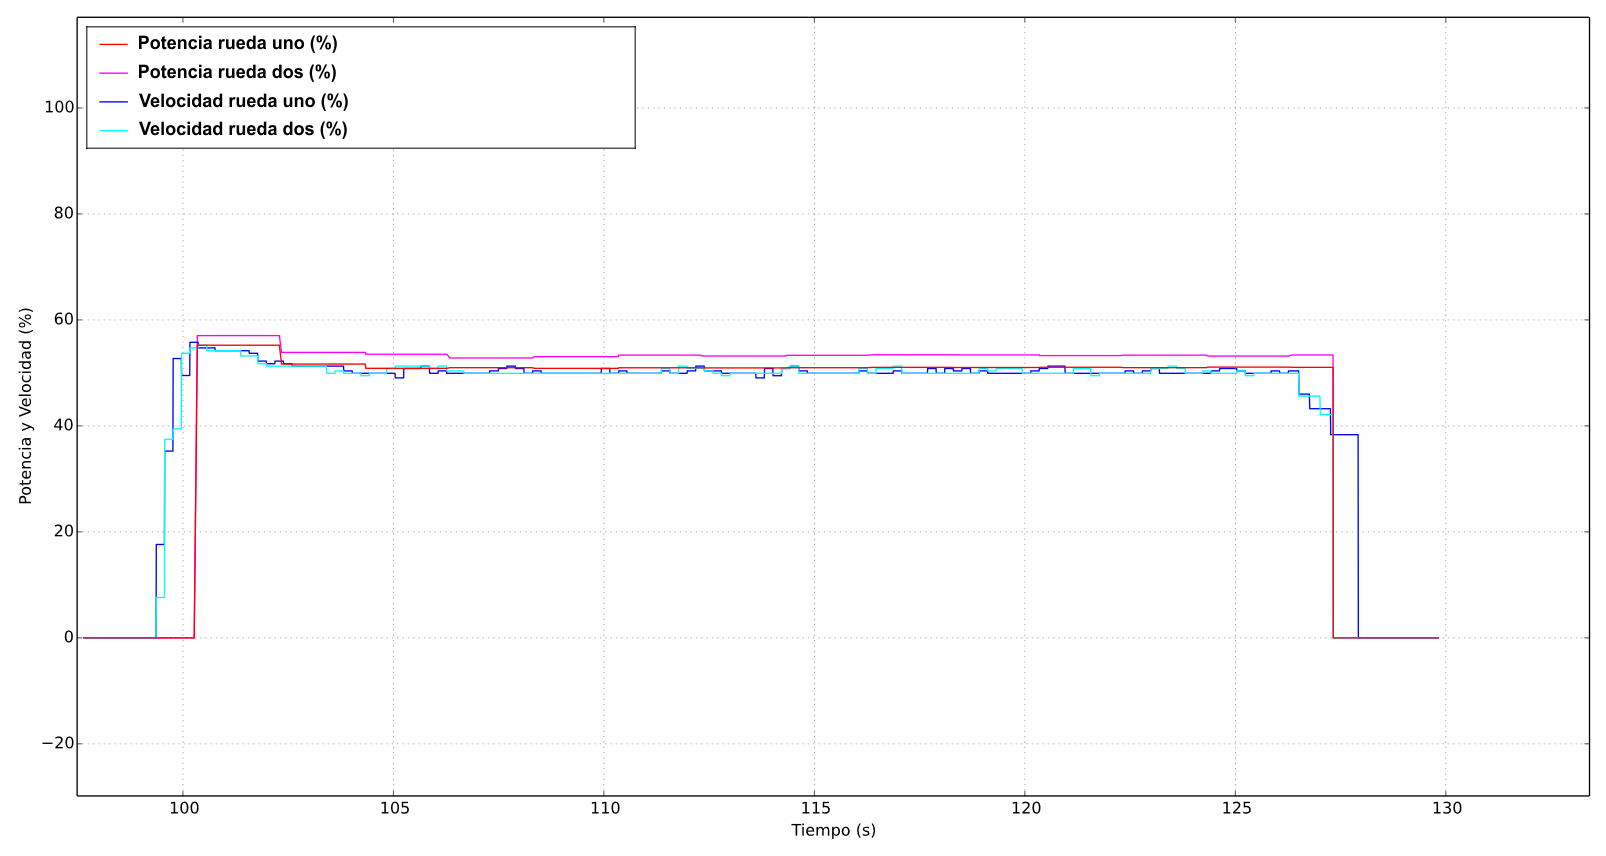
\includegraphics[width=0.5\textwidth]{images/Plot_ConstantPowvsSpeed}
  \caption[Prueba de Relación entre Potencia y Velocidad 2]{Relación entre potencia y velocidad con velocidades constantes.}
  \label{fig:plotConstantPowvsSpeed}
\end{figure}

En la figura \ref{fig:plotIncreasingPowvsSpeed} se observa el resultado de correr un script que envió comandos de velocidad crecientes hasta los valores máximos soportados por el hardware. Nótese que para la realización de este experimento se debió deshabilitar el mecanismo descrito en \ref{sec:Exp Eval :: Control Limite Velocidad}.

En la figura \ref{fig:plotConstantPowvsSpeed} se observa el resultado de correr un script que envió un comando de velocidad constante de \SI{1.50}{\metre/\second}, aproximadamente 50\% del máximo soportado.

De las dos gráficas anteriores se desprende que la relación entre potencia y velocidad es lineal, esto es, si se aplica un determinado porcentaje de la máxima potencia posible a los motores las ruedas alcanzaran una velocidad que sera similar en porcentaje respecto de la velocidad máxima posible. Visto esto, en las condiciones del experimento se recomienda que el parámetro que limita la desviación entre la potencia y la velocidad tenga un valor acotado. Se decidió admitir un desfajase del 25\%.

Realizado lo anterior, para probar el correcto funcionamiento del mecanismo de seguridad se realizaron 2 experimentos. En el primero se coloco un obstáculo (ladrillos) en el camino del robot de forma tal que para sortearlo el robot debiese aumentar la potencia enviada a los motores. En el segundo se coloco el robot con el frente apoyado contra un árbol (habiéndose desactivado el mecanismo de control de distancias), de forma que no pudiese avanzar al recibir ordenes para hacerlo. Se realizaron repeticiones de ambos experimentos a distintas velocidades (\SI{0.25}{\metre/\second}, \SI{0.50}{\metre/\second}, \SI{0.75}{\metre/\second}, \SI{1.00}{\metre/\second} y \SI{1.50}{\metre/\second}).

Para el primer experimento cuando se ordeno al robot avanzar a velocidades superiores a \SI{0.50}{\metre/\second} lograba sortearlo observándose un leve aumento en la potencia, para velocidades menores el robot se detuvo en el obstáculo requiriendo aumentar considerablemente la potencia para intentar alcanzar la velocidad objetivo y en este caso se disparó el mecanismo de seguridad deshabilitando el robot. Para el segundo experimento el robot siempre se deshabilitó inmediatamente después de ser habilitado y recibir ordenes de avanzar, habiéndose disparado el mecanismo de seguridad.

\section{Pruebas de Rendimiento}
\subsection{Throughput de la conexión TCP}
Se realizaron experimentos sobre la comunicación entre las placas \hl{SBC} e \hl{IO\_Board} buscando dimensionar el flujo de datos que es soportado en dicha comunicación.
Los experimentos consisten en monitorear y analizar los paquetes  de datos que se transmiten en la comunicación entre las placas considerando diferentes escenarios:
\begin{itemize}
	\item \textul{b\'{a}sico}: únicamente hay flujo de datos desde la \hl{IOBoard} a la \hl{SBC}, y dicho flujo corresponde a los reportes esenciales que realiza la placa para comunicar el estado de los motores (velocidades y potencias de los motores), así como también el estado general del robot y de sus mecanismos y dispositivos de seguridad.
	\item \textul{carga a 15hz}: contempla el flujo de datos del escenario anterior y agrega un tráfico de 15 mensajes por segundo, con la semántica de la funcionalidad \hl{ping}, enviados desde la placa \hl{SBC} a la placa \hl{IOBoard}, y al procesar estos mensajes esta última los responde generando un mensaje idéntico al recibido, lo que genera un flujo de daos extra desde la \hl{IOBoard} a la \hl{SBC} contemplando los reportes y todos los menajes de ping.
	\item \textul{carga a 30hz}: idéntico al escenario anterior pero generando 30 mensajes por segundo en lugar de generar 10.
	\item \textul{carga a 50hz}: idéntico al escenario anterior pero generando 50 mensajes por segundo en lugar de generar 30.
\end{itemize}
Es interesante analizar la cantidad de paquetes así como también la cantidad de datos que son procesados en la comunicación. A continuación se presentan gráficos representativos del flujo de paquetes, y cantidad de bits por segundo, que se analizaron por un período de 60 segundos aproximadamente y considerando las características de los escenarios descritos anteriormente.

\subsubsection{Escenario básico}
\begin{figure}[H]
  \centering
  	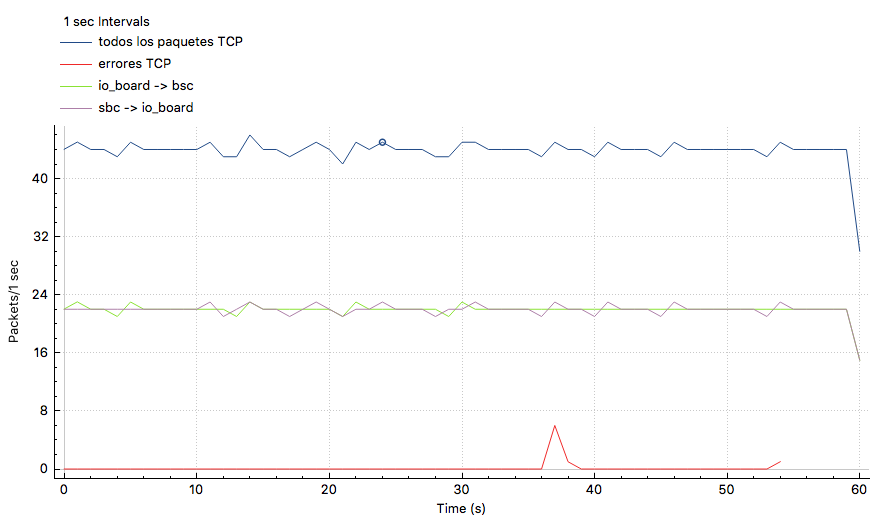
\includegraphics[width=0.8\textwidth]{images/TCP_Throughput_io_to_pc_basic_pkps}
  	\caption[Throughput de la conexión TCP - Básico]{Flujo de paquetes TCP en la comunicación SBC $\leftrightarrow$ IOBoard -  Escenario básico}
  \label{fig:TCP_Throughput_io_to_pc_basic_pkps}
\end{figure}

\begin{figure}[H]
  \centering
  	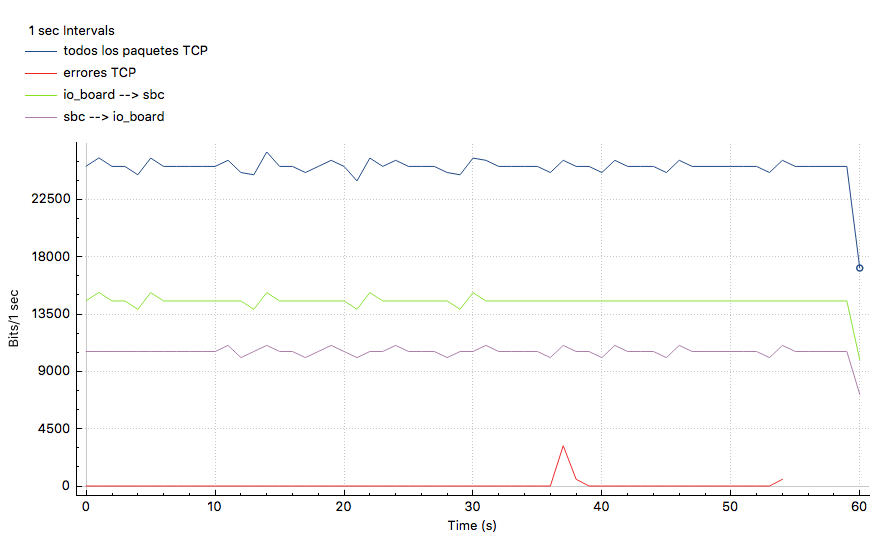
\includegraphics[width=0.8\textwidth]{images/TCP_Throughput_io_to_pc_basic_bps}
  	\caption[Throughput de la conexión TCP - Básico]{Flujo de datos (bits) TCP en la comunicación SBC $\leftrightarrow$ IOBoard -  Escenario básico}
  \label{fig:TCP_Throughput_io_to_pc_basic_bps}
\end{figure}
Se pueden observar los siguientes datos:
\begin{table}[H]
	\centering
 	\begin{minipage}[b]{0.6\textwidth}  	
  		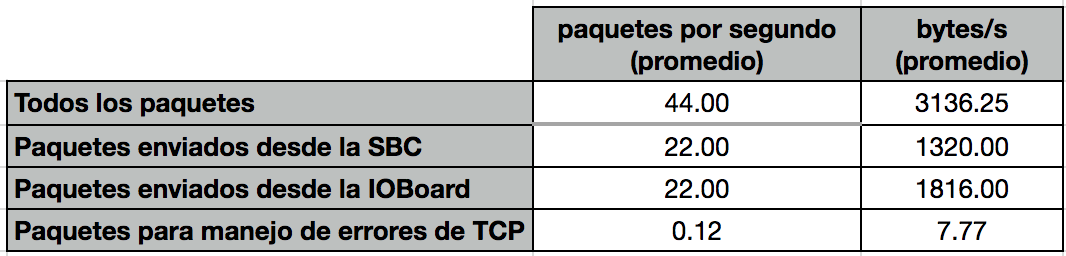
\includegraphics[width=\textwidth]{images/TCP_Throughput_io_to_pc_basic_results}
  		\caption[Throughput de la conexión TCP - Básico]{Flujo de paquetes TCP en la comunicación SBC $\leftrightarrow$ IOBoard -  Resultados en escenario básico}
		\label{fig:TCP_Throughput_io_to_pc_basic_pkps_results}
	\end{minipage}
\end{table}
Si bien se observa que la cantidad de paquetes que se envían desde cada placa son similares, esto es debido a que TCP exige confirmación de paquetes recibidos exitosamente, la cantidad de datos transmitidos es sensiblemente diferente para cada placa. Claro que esto tiene sentido ya que el flujo de datos es generado por los reportes de estados que realiza la placa de entrada/salida y la SBC simplemente responde confirmando que los mensajes fueron recibidos de forma correcta, siguiendo con la especificación del protocolo de comunicación.

También se observaron algunos mensajes de TCP utilizados para monitorear indicadores del protocolo, en particular los mensajes registrados en el experimento corresponden a alertas que indican la falta de confirmación de recibido a un mensaje. Estas alertas son de nivel de seguridad bajo y no se perdieron datos en la comunicación.

\subsubsection{Escenario con carga 15hz}
\begin{figure}[H]
  \centering
  	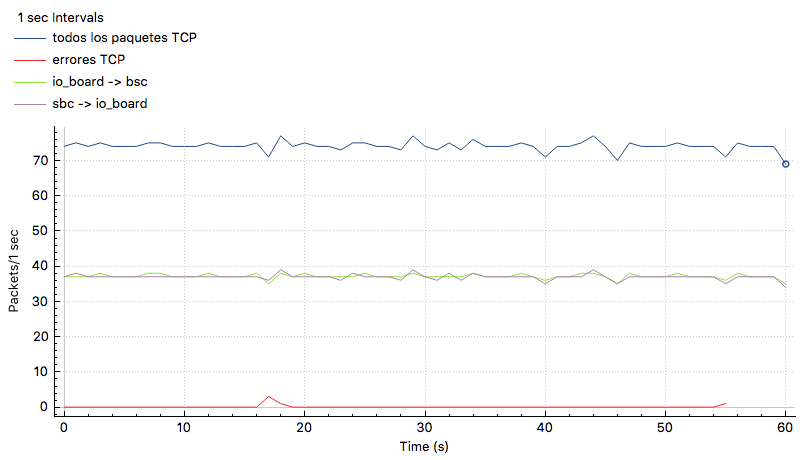
\includegraphics[width=0.8\textwidth]{images/TCP_Throughput_io_to_pc_15hz_pps}
  	\caption[Throughput de la conexión TCP - Escenario con carga a 15hz]{Flujo de paquetes TCP en la comunicación SBC $\leftrightarrow$ IOBoard -  Escenario con carga a 15hz}
  \label{fig:TCP_Throughput_io_to_pc_15hz_pps}
\end{figure}

\begin{figure}[H]
  \centering
  	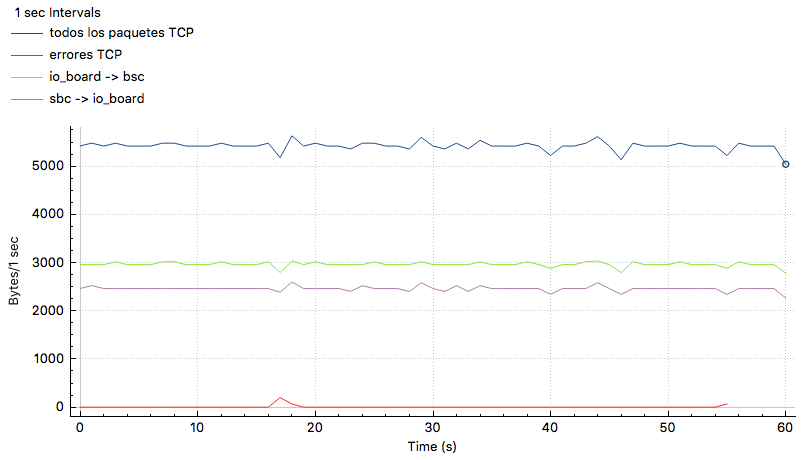
\includegraphics[width=0.8\textwidth]{images/TCP_Throughput_io_to_pc_15hz_bps}
  	\caption[Throughput de la conexión TCP - Escenario con carga a 15hz]{Flujo de datos (bits) TCP en la comunicación SBC $\leftrightarrow$ IOBoard -  Escenario con carga a 15hz}
  \label{fig:TCP_Throughput_io_to_pc_15hz_bps}
\end{figure}
Del experimento se observan los siguientes datos:
\begin{table}[H]
	\centering
 	\begin{minipage}[b]{0.6\textwidth}  	
  		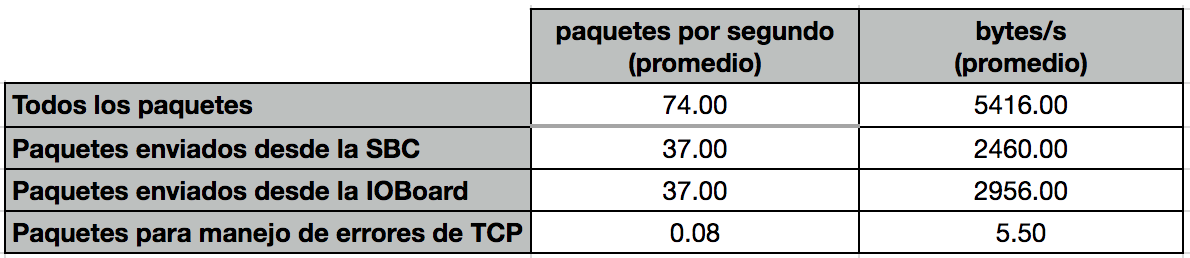
\includegraphics[width=\textwidth]{images/TCP_Throughput_io_to_pc_15hz_results}
  		\caption[Throughput de la conexión TCP - Escenario con carga a 15hz]{Flujo de paquetes TCP en la comunicación SBC $\leftrightarrow$ IOBoard -  Resultados en escenario con carga a 15hz}
		\label{fig:TCP_Throughput_io_to_pc_15hz_results}
	\end{minipage}
\end{table}

Como era de esperarse la cantidad total de paquetes por segundo aumenta en 30 paquetes respecto al escenario básico, esto es debido a que se generan 15 paquetes por segundo con el comando \textit{ping}, en la placa SBC, y los mismos son respondidos por la placa de entrada/salida ni bien llegan.
También en este escenario se registraron algunos paquetes de control de TCP para manejar algunos indicadores relevantes a la confirmación de entrega de paquetes. No se registra pérdida de datos en la comunicación.


\subsubsection{Escenario con carga 30hz}
\begin{figure}[H]
  \centering
  	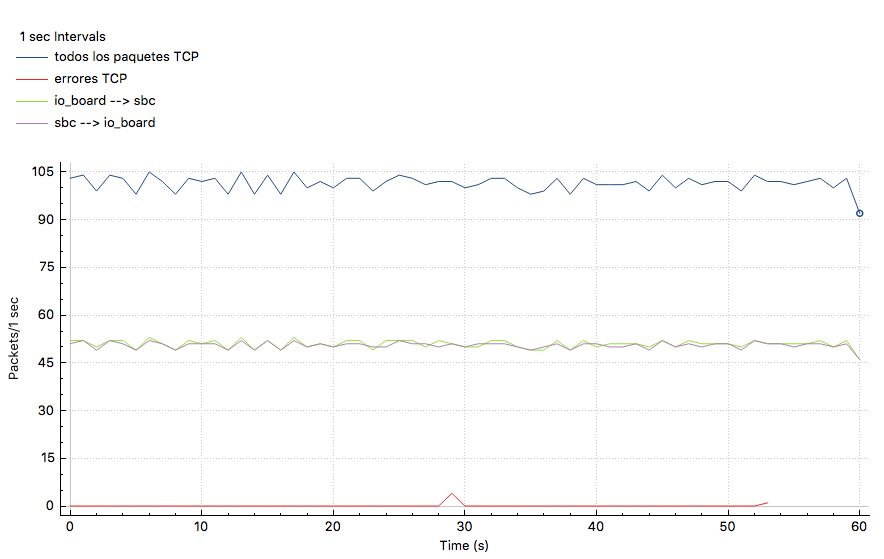
\includegraphics[width=0.8\textwidth]{images/TCP_Throughput_io_to_pc_30hz_pps}
  	\caption[Throughput de la conexión TCP - Escenario con carga a 30hz]{Flujo de paquetes TCP en la comunicación SBC $\leftrightarrow$ IOBoard -  Escenario con carga a 30hz}
  \label{fig:TCP_Throughput_io_to_pc_30hz_pps}
\end{figure}

\begin{figure}[H]
  \centering
  	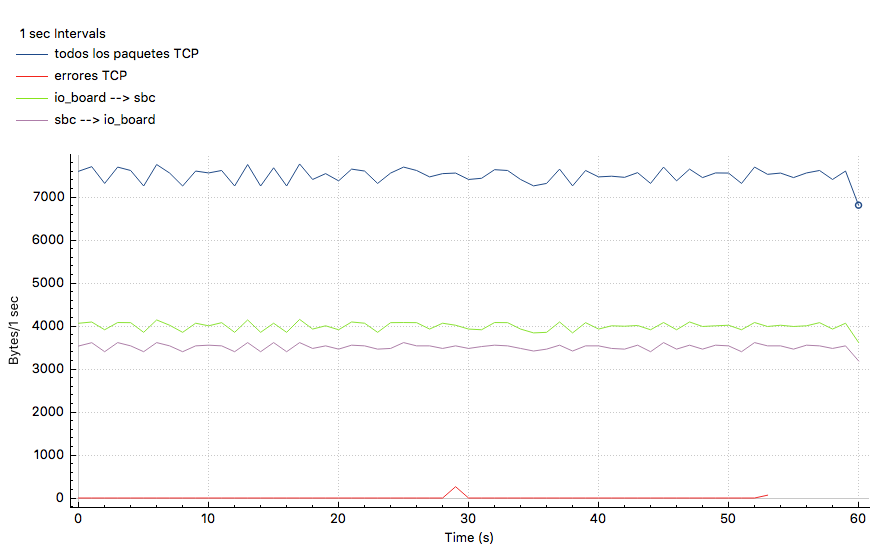
\includegraphics[width=0.8\textwidth]{images/TCP_Throughput_io_to_pc_30hz_bps}
  	\caption[Throughput de la conexión TCP - Escenario con carga a 30hz]{Flujo de datos (bits) TCP en la comunicación SBC $\leftrightarrow$ IOBoard -  Escenario con carga a 30hz}
  \label{fig:TCP_Throughput_io_to_pc_30hz_bps}
\end{figure}
Del experimento se pueden observar los siguientes datos:
\begin{table}[H]
	\centering
 	\begin{minipage}[b]{0.6\textwidth}  	
  		\includegraphics[width=\textwidth]{images/TCP_Throughput_io_to_pc_30hz_results}
  		\caption[Throughput de la conexión TCP - Básico]{Flujo de paquetes TCP en la comunicación SBC $\leftrightarrow$ IOBoard -  Resultados en escenario con carga a 30hz}
		\label{fig:TCP_Throughput_io_to_pc_30hz_results}
	\end{minipage}
\end{table}
Al igual que en el escenario anterior, se observa un aumento de flujo de datos consistente con el aumento de frecuencia de emisión de paquetes por la placa SBC con comandos \textit{ping}. 
También en este escenario se registra una cantidad insignificante de paquetes de control de TCP con procesamiento de alertas y no se registra pérdida de datos en la comunicación.


\subsubsection{Escenario con carga 50hz}
\begin{figure}[H]
  \centering
  	\includegraphics[width=\textwidth]{images/TCP_Throughput_io_to_pc_50hz_pps}
  	\caption[Throughput de la conexión TCP - Básico]{Flujo de paquetes TCP en la comunicación SBC $\leftrightarrow$ IOBoard -  Escenario con carga a 50hz}
  \label{fig:TCP_Throughput_io_to_pc_50hz_pps}
\end{figure}

\begin{figure}[H]
  \centering
  	\includegraphics[width=\textwidth]{images/TCP_Throughput_io_to_pc_50hz_bps}
  	\caption[Throughput de la conexión TCP - Básico]{Flujo de datos (bits) TCP en la comunicación SBC $\leftrightarrow$ IOBoard -  Escenario con carga a 50hz}
  \label{fig:TCP_Throughput_io_to_pc_50hz_bps}
\end{figure}
Del experimento se pueden observar los siguientes datos:
\begin{table}[H]
	\centering
 	\begin{minipage}[b]{\textwidth}  	
  		\includegraphics[width=\textwidth]{images/TCP_Throughput_io_to_pc_50hz_results}
  		\caption[Throughput de la conexión TCP - Básico]{Flujo de paquetes TCP en la comunicación SBC $\leftrightarrow$ IOBoard -  Resultados en escenario con carga a 50hz}
		\label{fig:TCP_Throughput_io_to_pc_50hz_results}
	\end{minipage}
\end{table}


\subsection{Tiempo de respuesta frente a situaciones anómalas (tiempo de deshabilitación)}
Con este experimento se pretendió tener una estimación del tiempo que insume el proceso de deshabilitación presentado en \hl{(Agregar ref a lugar donde se describe el proceso)} cuando alguno de los mecanismos de seguridad desarrollados indica que se esta en una configuración de peligro. El proceso de deshabilitación siempre es el mismo para todos los mecanismos de seguridad, por ello se decidió realizar el experimento utilizando solo uno de los mecanismos, en concreto, el mecanismo de control de distancias.

\begin{table}[H]  
  \centering
  \begin{minipage}[b]{0.4\textwidth}  	
  	\caption[Test Tiempo Deshabilitación]{Resultados de pruebas de tiempo de deshabilitación para diez ejecuciones.}
  	\includegraphics[width=\textwidth]{images/Test_DisablingTime}
  	\label{table:tableDisablingTimes}
  \end{minipage}
\end{table}

Como se observa en el Cuadro \ref{table:tableDisablingTimes} los tiempos de deshabilitación para cada experimento fueron prácticamente los mismos, lo cual es razonable considerando la implementación. En promedio el tiempo de deshabilitación es de \SI{1028.6}{\milli\second} $\cong$ \SI{1}{\second}.

%\subsection{Tiempos de respuesta en restablecer la conexión TCP}

\section{Evaluación de Resultados} \label{sec:Exp Eval :: Evaluación Resultados}
\subsection{Pruebas Funcionales}
\subsubsection{Control de Distancia}
Sobre el mecanismo de control de distancias: El mecanismo arrojó resultados satisfactorios. Considerando que a la máxima velocidad evaluada, \SI{1.50}{\metre/\second}, la distancia a la que se detuvo el robot fue, como se observa en el cuadro \ref{table:ultrasonic150}, de \SI{0.25}{\metre} en el peor caso; no es recomendable que el robot se desplace a velocidades superiores a esta máxima evaluada, esto al menos en las zonas que sean transitadas tanto por el robot como por humanos.
\subsubsection{Control de Límite de Velocidad}
Sobre el mecanismo de control del limite de velocidad: Los resultados arrojados por el mecanismo fueron los esperados, una vez la velocidad supera la máxima definida como segura el robot se deshabilita consistentemente en todas las situaciones.
\subsubsection{Control de la Relación entre Potencia y Velocidad}
Sobre el mecanismo de control de la relación entre potencia y velocidad: Si bien el mecanismo pudo ser validado y los resultados se muestran promisorios, las condiciones ideales en las que se realizo el experimento para determinar la relación entre la potencia y velocidad hacen que se deba ser cauto a la hora de tomar en cuenta estos resultados en otras circunstancias. Seria recomendable realizar experimentos que cubran mas situaciones y configuraciones que se asemejen más al ambiente final donde el robot operara. De hecho, por si solos los valores de velocidad y potencia aportan poca información acerca de lo que esta sucediendo, seria positivo contar con sensores que aporten mas información como podría ser la inclinación, el nivel de batería y el peso de la carga transportada por el robot.
\subsection{Pruebas de Rendimiento}
\subsubsection{Throughput de la conexión TCP}

\subsubsection{Tiempo de respuesta frente a situaciones anómalas (tiempo de deshabilitación)}
Sobre tiempo de respuesta frente a situaciones anómalas: Si bien se considera positivo que el tiempo de deshabilitacion sea constante, una demora de \SI{1}{\second} parece excesiva y da cabida situaciones de riesgo, habría optimizar el proceso. No obstante esto, si se sigue la recomendación realizada en esta misma sección de que el robot no se desplace a mas de \SI{1.50}{\metre/\second} el robot no colisionara con obstáculos aun con esta demora.

\hl{HAY QUE VER COMO ESTRUCTURAR Y REDACTAR MEJOR ESTAS EVALUACIONES}

\hl{GP: me parece mejor poner todos las evaluaciones en las secciones de pruebas y borrar esta secci\'{o}n}.

\chapter{Conclusiones y Trabajos Futuros}

En este último capítulo se presentan las conclusiones y trabajos a futuro.

\section{Conclusiones}
Este trabajo ha estado guiado durante su evolución por dos objetivos principales. El primero establecía la confección de una guía de seguridad como resultado del revelamiento de normas y estándares internacionales que hicieran foco en la seguridad aplicada a robots que realicen tareas colaborativas con humanos en ambientes laborales dinámicos y abiertos, mientras que el segundo establecía el desarrollo de un conjunto ``razonable'' de mecanismos de seguridad.

-Conclusiones sobre el primero objetivo.
-Conclusiones sobre el segundo objetivo.

\section{Trabajos Futuros}
Considerar los siguientes puntos:
Aún cuando la guía confeccionada sirve de apoyo a futuros desarrollos y los mecanismos implementados muestran resultados aceptables, existen varios puntos en los que se puede mejorar, o incluso abordar de forma completamente diferente a la realizada en el presente trabajo.
Se presenta a continuación los principales aspectos a desarrollar en trabajos futuros tomando como base los resultados obtenidos en el contexto de este proyecto.

\begin{itemize}
    \item Brake por hardware
    \item No se está controlando que el freno esté desactivado a la hora de establecer potencias a los motores luego de haber recibido un comando de velocidad. Si el freno estuviera posta lo que ocurriría en este caso es que se accionaría el control de potencia y desactivaría los motores debido a que no logra alcanzar una velocidad coherente con la potencia establecida.
    \item Enable por hardware controlado desde la ioboard para los motores
    \item Control de motores del chasis 2
    \item Conectar bocina
    \item Luz de emergencia encendida mientras el robot está alimentado de energía
    \item Control de ángulos máximos de giro (Para evitar choques entre chasis)
    \item Pruebas de los mecanismos de seguridad mas exhaustivas, en configuraciones ambientales mas variadas para evaluarlos mejor. La logística para acceder y mover el robot, el trabajar ``enchufados'', etc. dificultaron la realización de un mejor conjunto de pruebas.
\end{itemize}


%%%%%%%%%%%%%%%%%%%%%%%%%%%%%%%%%%%%%%%%%%%%%%%%%%%%%%%%%%%%%%%%%%%%%%%%%%%%%%%%
%% Bibliography:
%%
\cleardoublepage
\phantomsection
\addcontentsline{toc}{chapter}{Bibliografía}
\bibliographystyle{unsrt}
%\bibliographystyle{plainnat}
\bibliography{proyecto_ras.bib}


%%%%%%%%%%%%%%%%%%%%%%%%%%%%%%%%%%%%%%%%%%%%%%%%%%%%%%%%%%%%%%%%%%%%%%%%%%%%%%%%
%% Appendix:
%%

\appendix

\chapter{Información Adicional}


%%%%%%%%%%%%%%%%%%%%%%%%%%%%%%%%%%%%%%%%%%%%%%%%%%%%%%%%%%%%%%%%%%%%%%%%%%%%%%%%
%% Index:
%%
\printthesisindex
% Esto a continuación si quiero numerar las figuras desde 1.
%{%
%\let\oldnumberline\numberline%
%\renewcommand{\numberline}{\figurename~\oldnumberline}%
%\listoffigures%
%}

\listoffigures{}
\listoftables{}

\end{document}
